%-------------------------------------------------------------------------------
% This file provides a skeleton ATLAS document.
%-------------------------------------------------------------------------------
% \pdfoutput=1
% The \pdfoutput command is needed by arXiv/JHEP/JINST to ensure use of pdflatex.
% It should be included in the first 5 lines of the file.
%-------------------------------------------------------------------------------
% Specify where ATLAS LaTeX style files can be found.
\newcommand*{\ATLASLATEXPATH}{latex/}
%-------------------------------------------------------------------------------
%\documentclass[UKenglish,texlive=2011]{\ATLASLATEXPATH atlasdoc}
\documentclass[letterpaper,12pt,oneside,texlive=2015]{memoir} %The memoir class is great for longer works that use separate chapters. The Dissertation Office recommends 10-pt Arial or 12-pt Times New Roman. I use 12-pt for readability.
\usepackage[american]{babel} %Enables hyphenation and date formats according to American conventions. Change "american" to "british" (or another value) if you work outside the US.
\hyphenpenalty=750
\interfootnotelinepenalty=10000

\renewcommand\cftappendixname{\appendixname~}
\usepackage{todonotes}
\usepackage{amsfonts}
\usepackage{slashed}
\usepackage{braket}
\usepackage{hhline}
\usepackage{rotating}
\usepackage{multirow}
\usepackage{bm}

% \addto\captionsdutch{%
%   \renewcommand{\appendixname}%
%     {Appendix}%
% }
% \renewcommand*\cftappendixname{\appendixname}

% The language of the document must be set: usually UKenglish or USenglish.
% british and american also work!
% Commonly used options:
%  texlive=YYYY          Specify TeX Live version (2013 is default).
%  atlasstyle=true|false Use ATLAS style for document (default).
%  coverpage             Create ATLAS draft cover page for collaboration circulation.
%                        See atlas-draft-cover.tex for a list of variables that should be defined.
%  cernpreprint          Create front page for a CERN preprint.
%                        See atlas-preprint-cover.tex for a list of variables that should be defined.
%  PAPER                 The document is an ATLAS paper (draft).
%  CONF                  The document is a CONF note (draft).
%  PUB                   The document is a PUB note (draft).
%  txfonts=true|false    Use txfonts rather than the default newtx - needed for arXiv submission.
%  paper=a4|letter       Set paper size to A4 (default) or letter.

%-------------------------------------------------------------------------------
% Extra packages:
\usepackage{\ATLASLATEXPATH atlaspackage}
% Commonly used options:
%  biblatex=true|false   Use biblatex (default) or bibtex for the bibliography.
%  backend=biber         Use the biber backend rather than bibtex.
%  subfigure|subfig|subcaption  to use one of these packages for figures in figures.
%  minimal               Minimal set of packages.
%  default               Standard set of packages.
%  full                  Full set of packages.
%-------------------------------------------------------------------------------
% Style file with biblatex options for ATLAS documents.
\usepackage{\ATLASLATEXPATH atlasbiblatex}

% Package for creating list of authors and contributors to the analysis.
\usepackage{\ATLASLATEXPATH atlascontribute}
\usepackage{\ATLASLATEXPATH atlascover}

% Useful macros
\usepackage{\ATLASLATEXPATH atlasphysics}
\usepackage{\ATLASLATEXPATH atlasheavyion}
% See doc/atlas-physics.pdf for a list of the defined symbols.
% Default options are:
%   true:  journal, misc, particle, unit, xref
%   false: BSM, hion, math, process, other, texmf
% See the package for details on the options.

% Files with references for use with biblatex.
% Note that biber gives an error if it finds empty bib files.
\addbibresource{thesis.bib}
\addbibresource{bibtex/bib/ATLAS.bib}
\addbibresource{bibtex/bib/CMS.bib}

\addbibresource{bibtex/bib/ConfNotes.bib}
\addbibresource{bibtex/bib/PubNotes.bib}

\setlength{\bibitemsep}{\baselineskip} %Skip lines between bibliography entries. Columbia requires that you skip a line between entries.

% Paths for figures - do not forget the / at the end of the directory name.
\graphicspath{{logos/}{figures/}}

% Add you own definitions here (file thesis-defs.sty).
\usepackage{thesis-defs}

%% comment this out for final version
\usepackage{lineno}
\linenumbers

\let\newfloat\undefined
\usepackage{floatrow}
\floatsetup[table]{capposition=bottom}
\floatsetup[figure]{capposition=bottom}


\makeatletter
\g@addto@macro\@floatboxreset\centering
\makeatother

\usepackage{cleveref}
\Crefname{equation}{Eq.}{Eqs.}
\Crefname{align}   {Eq.}{Eqs.}
\Crefname{figure}{Fig.}{Figs.}
\Crefname{tabular}      {Table}{Tables}
\Crefname{sidewaystable}{Table}{Tables}
\Crefname{table}        {Table}{Tables}
\Crefname{section}{Sec.}{Secs.}
\Crefname{chapter}{Ch.}{Ch.}
\Crefname{appendix}{App.}{App.}
\Crefname{subsection}{Sec.}{Secs.}

%-------------------------------------------------------------------------------
% Generic document information
%-------------------------------------------------------------------------------

% Author and title for the PDF file
\hypersetup{pdftitle={ATLAS Thesis},pdfauthor={Michael (Felix) R. Clark}}

%-------------------------------------------------------------------------------
% Content
%-------------------------------------------------------------------------------
%Dissertation Template for Columbia University Ph.D. programs
%By Charles McNamara, 2015
%I posted this document under a CC0 public domain license -- do whatever you want with it!
%It's probably a good idea to review the university guidelines just so you know what you want your dissertation to look like. You can read about those guidelines at this site: http://gsas.columbia.edu/content/formatting-guidelines.
%Good luck writing your dissertation!


% This is the main document file for the dissertation. You should not include any of your actual chapters or other substantive writing in this file.
%First we have to set up the style and formatting of the pages.

%\setmainfont{Linux Libertine O} %This is a really readable serif font. It renders polytonic Greek better than any other OpenType font I've found, including Times New Roman. I now use it for everything, including class handouts. Highly recommended for classicists.


%Here is some stuff on the bibliography. You want to keep your bibliography file in the same directory as this file.

%\usepackage[backend=bibtex8,style=authoryear-icomp,texencoding=utf8,bibencoding=utf8]{biblatex} %The command here uses biblatex to render your bibliography, and it tells biblatex to use Unicode fonts. You can change the style of your citations easily by changing the value for "style" -- I use authoryear-icomp which takes care of the id/ibid citations automatically. There are many styles available if you want to change it.
%I have tried to use biber instead of biblatex many times, but it's never worked properly for me. I use biblatex, but feel free to try biber instead.

%\addbibresource{./Bibliography.bib} %Your bibliography file. I use JabRef to keep track of my bibliography. Highly recommended, and free! You can use Zotero if you want, but I've had trouble exporting to .bib files from my Zotero database.


%Here you can set margins and other page formatting

\setlrmarginsandblock{3.175cm}{3.175cm}{*} %Left and right margin -- the dissertation office requires at least 1-inch margins
\setulmarginsandblock{2.54cm}{2.54cm}{*}  %Upper and lower margin -- same thing, at least 1-inch margins
\checkandfixthelayout %A function of the memoir class that finds the right number of lines per page and apparently tidies up the formatting in other mysterious ways...?

% Below we start to set up the document itself, including how to use spacing throughout the dissertation.

\begin{document}

\sloppy %If I don't include sloppy, then Greek and Latin words screw up margins all over. If you don't include weird languages in your dissertation, you can probably leave this one out.
\chapterstyle{chappell} % Nice formatting for chapter headings. Check out the documentation for the memoir class for other options.
\footnotesep\baselineskip % Footnotes need to have a space between each one for Columbia's Dissertation Office.
\DoubleSpacing %Set roomier body text throughout your writing. The dissertation office requires that you use double-spacing throughout your main body text.
\expandafter\def\expandafter\quote\expandafter{\quote\SingleSpace} %Keep all block quotes single-spaced regardless of body text spacing.
\pagestyle{plain} %Put page numbers at the bottom-center for the whole dissertation. Columbia's dissertation office requires that the numbers appear at this location on the page throughout the document.

\newcommand{\thesisTitle}{Signatures of hydrodynamics  in $\sqrt{s_\mathrm{NN}} = 5.02~\TeV$ proton-lead collisions using femtoscopy with the ATLAS detector at the Large Hadron Collider}
\newcommand{\myName}{Michael R. Clark}
\newcommand{\abstractText}{
abstract text here
}
\newcommand{\yearText}{2018}
%The section that follows renders the "Cover pages and Abstract" part of your dissertation.

%We need to define a customized command to render Columbia's required title page
%Be sure you replace the title and author with the title of your dissertation and your name!
\newcommand*{\TitleColumbia}{\begingroup
\begin{center}
\thesisTitle{} \\
\myName{} \par
\vspace*{5 in} %This is a sloppy way to get the "Submitted in partial fulfillment" part to move to the bottom of the page
%\begin{SingleSpace} can be used here if you want the "Submitted" text to be single-spaced.
Submitted in partial fulfillment of the\\
requirements for the degree of\\
Doctor of Philosophy\\
in the Graduate School of Arts and Sciences\par
%\end{SingleSpace} here if you decide to use single-spacing on the "Submitted" text.
\vfill
COLUMBIA UNIVERSITY\\
\yearText
\end{center}
\endgroup}

%These four commands make sure that your title page doesn't count toward your page number counts and that there is no extra header and footer on the page. The final command here also renders the page as you've defined it above.
\pagenumbering{gobble}
\clearpage
\thispagestyle{empty}
\TitleColumbia

%What follows is the copyright page
%We make sure that LaTeX moves to the next page, doesn't use page numbers, and doesn't include any headers or footers.
\newpage
\pagenumbering{gobble}
\clearpage
\thispagestyle{empty}
\begin{center}
\vspace*{7.5 in} %Another sloppy way to get the copyright notice to move to the bottom of the page.
© \yearText{} \\
\myName{} \\
All rights reserved
\end{center} %There are lots of copyright options available for your dissertation, including Creative Commons licensing. You should scope out Columbia's Dissertation Office website for more information.

%Now we need the abstract
%Again, we prevent page numbers and headers and footers from appearing on this page.
\newpage
\pagenumbering{gobble}
\clearpage
\thispagestyle{empty}
\begin{center}
ABSTRACT\\ %You need to keep this text here in all capitals. Don't change it.
\thesisTitle \\ %Do of course change this to the title of your dissertation.
\myName \\ %Your name here
\end{center}
\abstractText{}

%Phew, you're done with the "Cover pages and abstract" part. Now to the "Prefatory pages."
\frontmatter %This command lets LaTeX know that you want lowercase Roman page numbers in these next sections.

\tableofcontents* %LaTeX automatically renders your table of contents using your \chapter and \section commands throughout the whole document. If you don't want something to appear in the table of contents, simply use an asterisk in the command, like \chapter*{} or \section*{}

%include lists of figures and tables
\newpage
\listoffigures
\newpage
\listoftables

%Here I need an acknowledgments page.
%\newpage
\chapter{Acknowledgments} %I use an asterisk because I don't want my acknowledgements in the table of contents. I use \chapter to make sure that the acknowledgements go on the correct side of the page when you print out the dissertation.

acknowledgments go here

%% to my parents, my first teachers 
%% brian, bill
%% postdocs: aaron, soumya, sarah, martin
%% fellow physics grad students: laura, russell, ryne, josh, matt, zach (other group members)
%% Brad, Devon, and Leah
%% Kate
%% Grandma June & GG & grandparents
%% etc.


%\newpage
\chapter*{Dedication} %Same here -- asterisk so that my dedication doesn't show up in the table of contents. You might want to take out "Dedication" as the title of this chapter. It's just here for a placeholder.
\vfil
\begin{center}
{\large \textit{To Mick \\ and Janice}}
\end{center}
\vfil



%What follows is the main text of your dissertation. You can comment out lines if you want to exclude them from your document for drafts. Everything after \mainmatter will get Arabic numbers centered on the bottom of the page.

\mainmatter

%I use subdirectories for each part of my dissertation just to keep the files tidy. LaTeX generates a lot of different files for output, and using subdirectories allows you to find your .tex files more easily.

\chapter{Introduction}
\label{ch:intro}

%% quotes to potentially sprinkle:
%% intro: ``In the beginning the Universe was created. This has made a lot of people very angry and been widely regarded as a bad move.'' -- Douglas Adams
%% acknowledgements: ``Getting an education was a bit like a communicable sexual disease. It made you unsuitable for a lot of jobs and then you had the urge to pass it on.'' -- Terry Pratchett
%% theory lol: ``I can believe things that are true and things that aren't true and I can believe things where nobody knows if they're true or not.'' -- Neil Gaiman
%% or: ``Maturity, one discovers, has everything to do with the acceptance of 'not knowing'.'' -- Mark Z. Danielewski
%% results: ``The most exciting phrase to hear in science, the one that heralds new discoveries, is not 'Eureka!', but 'That's funny...'' --- Isaac Asimov

 notes:

 we see collectivity in even fairly low multiplicity pp, and it doesn't look particularly like hydro (?) (see Z-tagged pp v2). refer to AMPT (, CGC ?) models that predict v2 in pp. this thesis will argue that the collectivity in central \pPb has specific features that suggest hydro -- it's not clear in low multiplicity.

 
why HI physics? %% \cite{Busza:2018rrf} for big picture, but no citations in intro?
cosmology, very early universe. HI collisions are ``little bangs''
phase diagram of \qcd -- essentially phase diagram of \emph{matter}
how does strongly-coupled fluid emerge from constituents that are weakly-coupled at short length scales?


\Cref{ch:background} discusses the historical background of nuclear physics and some of the developments made in the study of heavy ion collisions.
It also introduces the framework for understanding femtoscopic measurements in general.
\Cref{ch:experiment} motivates the some of the design for high-energy collider experiments and describes several components of the \ac{LHC} and the ATLAS detector.
The process of reconstructing charged particles and identifying pions is discussed in \cref{ch:reconstruction}.
\Cref{ch:analysis} provides the details of the measurement process for the analyses and enumerates the systematic effects and uncertainties.
The results of the ATLAS femtoscopy measurements in \pPb collisions are presented with discussion in \cref{ch:results}, including some comparisons to theoretical hydrodynamic models.
       % Introduction
\chapter{Theoretical and phenomenological background}
\label{ch:background}
\graphicspath{{Chapter-Background/figures/}}

\section{Quantum chromodynamics}
\subsection{History and experimental motivation}

The atomic nucleus was discovered in the early 20th century \cite{Rutherford:1911zz}, and a few years later it was determined that it was composed of protons ($p$).
An additional, electrically-neutral nuclear constituent particle was proposed soon after and the neutron ($n$) was finally discovered in the early 1930s \cite{Chadwick:1932ma}.
Clearly some new type of interaction, strong enough to overcome electrostatic repulsion between protons, bound the nucleons ($p$ and $n$) together in the nucleus.
A particle field was proposed to mediate this strong interaction, dubbed the pion ($\pi^\pm$, $\pi^0$) \cite{Yukawa:1935xg}.
Since the strong interaction only acts over a length scale of about 2 fm, the mediating pion was predicted to have a mass of about 100 \MeV\footnote{The potential mediated by a boson of mass $m$ is proportional to \( - \exp(-mcr/\hbar)/r\), where $r$ is the separation between a pair of participants. Thus the mass of a mediating boson for a potential with a characteristic cutoff length of $\lambda$ is $m = \hbar/c\lambda = \frac{200 \MeVcc \textrm{fm}}{\lambda}$.}.
The charged pion was indeed discovered experimentally in 1947 \cite{Lattes:1947mw}.
Pions can be interpreted as the Nambu-Goldstone bosons corresponding to the spontaneously broken chiral symmetry, which explains their relatively small masses.

The expanding body of observed hadrons --- particles bound by the strong nuclear interaction --- and the allowed decays thereof suggested additional conserved quantum numbers suggested that they could be composed of constituent particles.
It was noticed that hadrons can be organized by their quantum numbers in a manner described by an $SU(3)$ \emph{flavor} symmetry \cite{GellMann:1962xb}.
This suggests that hadrons are composed of constituent particles called \emph{quarks}, each with a quantum number called flavor that can takes a value of ``up'' ($u$), ``down'' ($d$), or ``strange'' ($s$)\footnote{Three heavy flavors have since been discovered, ``charm'' ($c$), ``bottom'' ($b$), and ``top'' ($t$), but heavy quarks and the hadrons composed of them decay very rapidly due to their larger mass.}.
The quark model was not immediately accepted because free quarks were not (and still have not been) observed.
Scattering experiments were needed to probe the internal structure of hadrons.

Because electrons are point-like particles to the limits of current experiments, a scattering process $e^- A \rightarrow e^- X$ is dependent only on the internal structure of the target $A$.
The electron scatters through a virtual photon that interacts directly with the hadron in a process called \ac{DIS}\footnote{``deep'' because it probes the constituent structure of the target, ``inelastic'' because kinetic energy and matter are exchanged in the creation of the product particles}.
The kinematics of the electron in type of experiment constrain the structure of the target hadrons.

\begin{figure}[t]
  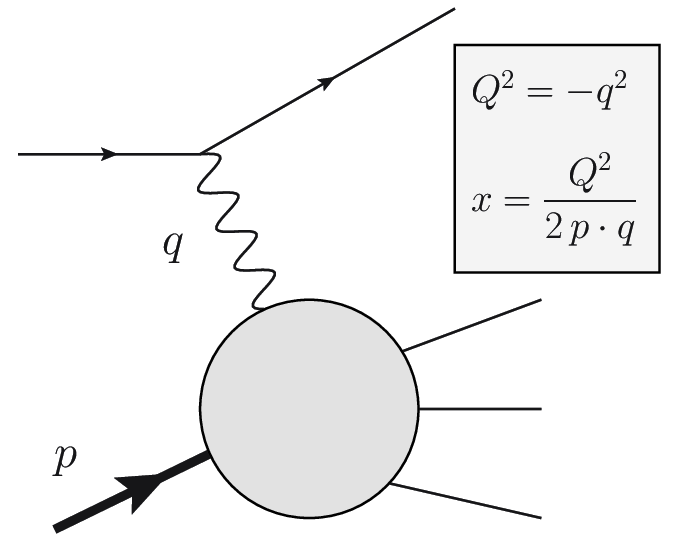
\includegraphics{dis_electron_proton.png}
  \caption{Deep inelastic scattering of a lepton on a hadron \cite{dis_fig_proceedings}.}
  \label{fig:dis}
\end{figure}

Under the constraints of Lorentz and gauge invariance, the cross-section of an unpolarized \ac{DIS} process with incoming lepton and proton momenta $k$ and $P$ respectively and momentum transfer $q$ can be expressed as \cite{Tanabashi:2018oca}
\begin{equation}
  \frac{d^2 \sigma}{dx \, dQ^2} = \frac{4\pi\alpha^2_\textrm{EM}}{2xQ^4}\left[ \left(1+(1-y)^2\right) F_2\left(x, Q^2\right) - y^2 F_L \left(x, Q^2\right) \right]
  \label{eq:dis}
\end{equation}
where $Q^2 = -q^2$ is the absolute magnitude squared of the photon's virtuality, $x = \frac{Q^2}{2q \cdot P}$, and $y = \frac{q \cdot P}{k \cdot P}$ is the fraction of the lepton's energy lost in the nucleon's rest frame.
In the parton model, which describes the proton as approximately-free point-like quarks in the infinite longitudinal momentum frame, $x$ is interpreted as the fraction of the target proton's momentum carried by a struck parton.
The structure functions $F_i(x, Q^2)$ describe the inherent internal structure of the proton.
The longitudinal structure function $F_L = F_2 - 2xF_1$ is zero by the Callan-Gross relation \cite{Callan:1969uq}, and experimentally the ratio $2xF_1 / F_2$ is consistent with 1 independent of $x$.
In the parton model, where the proton is described in terms of free point-like quarks constituents, the structure function $F_2$ is decomposed into \acp{PDF}
\begin{equation}
F_2 \left(x, Q^2\right) = x \sum_q e_q^2 f_{q/p}(x)
\end{equation}
to lowest order in the strong coupling constant $\alpha_s$.
The independence of $Q^2$ of the \acp{PDF} is a manifestation of their point-like description in the parton model and is known as \emph{Bjorken scaling}.
Logarithmic corrections are understood theoretically and arise as gluon radiation from the quarks becomes relevant, particularly at small $x$ (\cref{fig:proton_f2}).

\begin{figure}[t]
  %% page 326 of particle review
  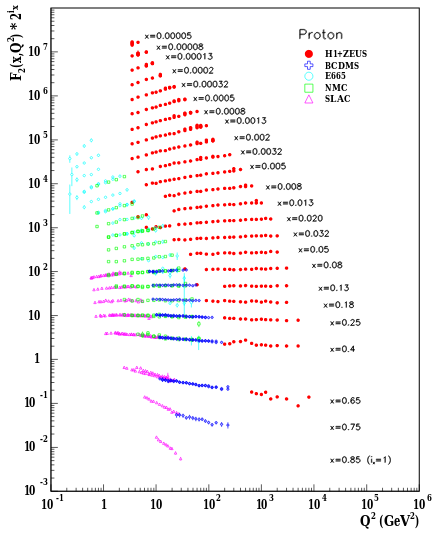
\includegraphics[width=0.45\linewidth]{proton_f2.png}
  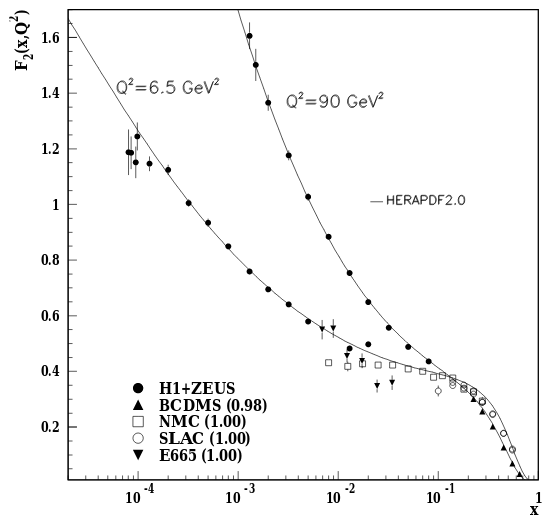
\includegraphics[width=0.54\linewidth]{proton_f2_vs_x.png}
  \caption{The structure function $F_2\left(x, Q^2\right)$ of the proton as a function of $Q^2$ (left) and of $x$ (right) \cite{Tanabashi:2018oca}.}
  \label{fig:proton_f2}
\end{figure}

An experimental and phenomenological description of the nucleon structure functions does not provide a complete description of the interactions among nucleon constituents.
The success of gauge theories in describing \ac{QED} ($U(1)$) and electroweak theory ($U(2) = SU(2) \otimes U(1)$) suggests that some other gauge theory may be able to describe the nuclear interaction.
A quantum field theory with an $SU(N_c)$ ``color'' symmetry with $N_c$ colors, called \qcd, is one such candidate.
For it to be a believable description of the strong interaction, it must not only be consistent with experimental observations, but it must also explain why free quarks have never been observed.
The rate of hadronic production in electron-positron collisions is proportional to $N_c$, so experimental measurements of the ratio\footnote{at energies above the $b\bar{b}$ threshold and below the mass of the $Z$ boson}
\begin{equation}
R \equiv \frac{\sigma\left(e^+ e^- \rightarrow \textrm{hadrons}\right)}{\sigma\left(e^+ e^- \rightarrow \mu^+ \mu^- \right)} \approx N_c \sum_{q \in \{u,d,s,c,b\}} e_q^2 = \frac{11}{9} N_c
\end{equation}
have been made to determine the number of colors, showing very good agreement with a value of $N_c = 3$.
Though the non-abelian character of \qcd makes many practical calculations difficult, it has shown remarkable success in describing the strong interaction, as will be discussed in the remainder of this section.

\subsection{The QCD Lagrangian}
The gauge-invariant lagrangian density of \qcd \cite{Wilczek:2000ih} is that of an $N_c=3$ Yang-Mills theory given by
\begin{equation}
  \Lagr_\mathrm{QCD} \equiv -\frac{1}{4} G^a_{\mu\nu}G^{a\mu\nu} + \bar{\psi} \left( i \slashed{D} - m \right) \psi \; .
\end{equation}
Here repeated indices are summed, where $\mu$ and $\nu$ indicate spacetime indices, $a$, $b$, and $c$ indicate color indices in the fundamental ($N=3$) representation, and $A$, $B$, and $C$ indicated color indices in the adjoint ($N=8$) representation.
The slash notation refers to contraction with the gamma matrices $\{\gamma^\mu, \gamma^\nu\} = 2\eta^{\mu\nu}$\footnote{with Minkowski signature $(+---)$}.
The covariant derivative
\[ D_\mu \equiv \partial_\mu - i g A^C_\mu t^C\]
where $A^C_\mu$ is the gluon field, $t^C$ are the generators of the $SU(3)$ gauge group, and $g$ is the strong charge constant.
The constant $g$ in the lagrangian is always squared when computing rates from quantum amplitudes, so physical results are typically expressed in terms of
\begin{equation}
  \alpha_s \equiv \frac{g^2}{4\pi} \; ,
\end{equation}
typically called the strong coupling constant.
The gluon field strength tensor is
\[ G^A_{\mu\nu} \equiv \partial_\mu A^A_\nu - \partial_\nu A^A_\mu + g f^{ABC} A^B_\mu A^C_\nu \]
with the $SU(3)$ structure constants defined such that
\[ [t^A,t^B] = if^{ABC}t^C \; \footnote{In the $SU(2)$ gauge group the adjoint representation is three-dimensional and the structure constants are given by the anti-symmetric Levi-Civita symbol $\epsilon^{ABC}$}.\]
The quark fields are defined such that the mass matrix $m$ is diagonal:
\[ \bar{\psi}m\psi = \sum_{q = u,d,s,\ldots} m_{q}\bar{q}q \]
The quark masses $m_q$ are generated by the mechanism of spontaneous electro-weak symmetry breaking in which the Higgs field, coupling to fermions and electro-weak gauge bosons, acquires a nonzero vacuum expectation value.
This procedure induces in the \qcd vacuum a breaking of the chiral symmetry $SU(N_f) \times SU(N_f) \rarrow SU(N_f)$ in the massless Lagrangian.

\begin{figure}[t]
  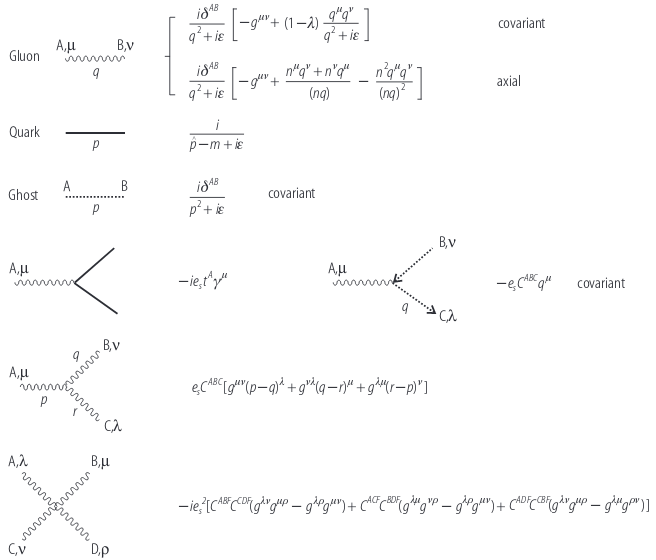
\includegraphics{qcd_feynman.png}
  \caption{The propagators and vertices in QCD along with the corresponding Feynman rules for the amplitude factors \cite{Altarelli:2013tya}. The strong coupling charge is written here as $e_s = \sqrt{4\pi\alpha_s}$, and the gauge parameter is denoted by $\lambda$.}
  \label{fig:qcd_feynman}
\end{figure}

%% The QCD Lagrangian has a symmetry under the gauge transformation defined as... %% we don't really need to get explicit about gauge transformations
The physical interaction vertices of \qcd are a 3-point quark-gluon vertex analogous to he \ac{QED} vertex, a 3-gluon vertex and a 4-gluon vertex (\cref{fig:qcd_feynman}).
A scalar ghost field\footnote{which has a spin of 0 yet anti-commutes like a fermion} also couples to the gluon as is generally necessary in non-abelian gauge theories to prevent over-counting gauge-equivalent states \cite{Faddeev:1967fc}.
The non-abelian nature of \qcd manifests in Feynman diagrams as the gluon self-interaction vertices.
The gluon-gluon interactions make \qcd difficult to calculate with.
In a classical theory, they prevent the principle of superposition from being applied in chromodynamics.
The highly-nontrivial gluon self-interaction is a crucial ingredient in the richness of nuclear physics.


\subsection{Running of the coupling constant} %% maybe doesn't deserve its own section, instead split into UV and IR?

%% https://arxiv.org/pdf/1604.08082.pdf

As is the case in all quantum field theories, the na\"ive calculation of higher-order (in $\alpha_s$) loop diagram integrals contain divergences in the amplitudes.
In many theories, including \qcd \cite{Gross:1973ju}, these infinities can be dealt with with a process called \emph{renormalization}.
One description of renormalization is the introduction of an energy/momentum cutoff scale.
Physical calculations cannot depend on any such scales, so amplitude calculations must be organized such that any dependence on the renormalization scale cancels in a physical result, which can be done order-by-order in perturbation theory.
This process induces a scale dependence of the coupling constant $\alpha_s$ on the arbitrary renormalization scale $\mu$.
If the value of $\alpha_s$ is known at a particular $\mu = \mu_0$, its dependence on the scale can be determined by calculating the beta function
\begin{equation}
  \beta(\alpha_s) \equiv  \frac{\partial \alpha_s}{\partial \ln \mu^2}
\end{equation}
which to one loop is given by \cite{Gross:1973id}
\begin{equation}
  \beta(\alpha_s) = -b_0 \alpha_s^2 + \bigo{\alpha_s^3}
\end{equation}
where
\[
%% \beta_1 = \frac{11 N_c - 2 N_f}{3}
b_0 = \frac{11 N_c - 2 N_f}{12\pi}
\]
for $N_c$ colors and $N_f$ relevant quark flavors at the scale of the process.
The \ac{LO} solution is
\begin{equation}
  \alpha_s(\mu^2) = \frac{1}{b_0 \ln\left(\mu^2 / \lqcd^2\right)}
  \label{eq:running_as}
\end{equation}
where \lqcd is defined by a given value for $\alpha_s$ at a scale $\mu_0$
\[
\lqcd = \mu_0 \exp \left( -\frac{1}{2 b_0 \alpha_s(\mu_0^2)} \right) \; .
\]
The above expression for \lqcd changes depending on the order of the perturbative expansion and the renormalization scheme, but the physical meaning of \lqcd is still apparent.
It is the energy scale below which the strong coupling diverges, showing an explicit breakdown of perturbation theory.
It is noteworthy that \qcd predicts the emergence of such a scale, even in the conformal\footnote{i.e. a scale-invariant lagrangian with massless quarks} theory.
Practically the \qcd scale is often quoted around a value of %% at the 5-quark level, where \mu ~ m_Z
\[
\lqcd \approx 200 \MeV \;,
\]
but the precise value can differ by a factor of 2 or more depending on arbitrary choices such as scheme, order, and gauge.

A convenient choice for the renormalization scale $\mu$ in \cref{eq:running_as} is to set $\mu^2 = Q^2$ for a physical process with momentum transfer $Q$.
This choice introduces some theoretical and computational wrinkles but gives a simple and direct relationship to experimental data.
Experimental values of the strong coupling constant are typically reported at the mass of the $Z$ boson, with a current world average value of
\[
\alpha_s(m_Z^2) = 0.1181 \pm 0.0011
\]
where $m_Z = 91.187 \GeV$.
The running of the coupling is demonstrated by the summary of experimental measurements in \cref{fig:running_coupling}.

\begin{figure}[t]
  %% page 155 of particle review
  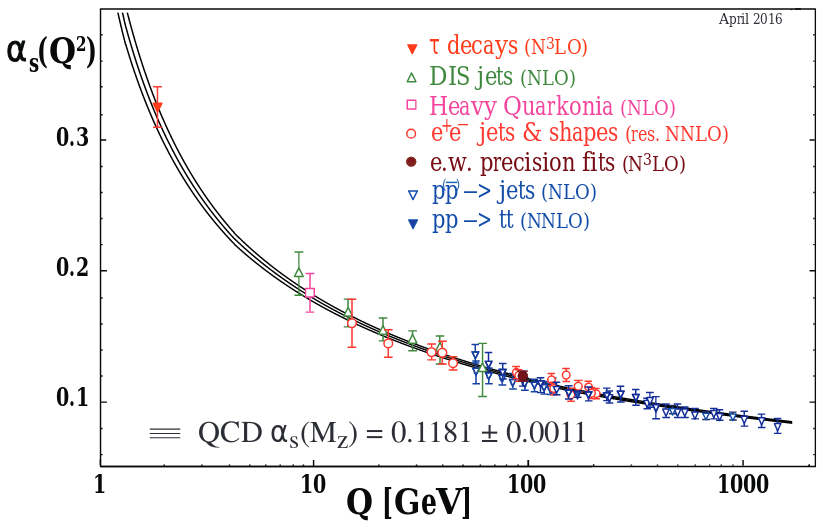
\includegraphics{running_as.png}
  \caption{Measurements of the strong coupling constant $\alpha_s$ as a function of the energy scale $Q$ \cite{Tanabashi:2018oca}.}
  \label{fig:running_coupling}
\end{figure}

\subsection{Asymptotic freedom}

The strong coupling constant decreases with rising energy as shown in \cref{eq:running_as} and \cref{fig:running_coupling}.
This phenomenon is known as \emph{asymptotic freedom} and is necessary to explain Bjorken scaling, since without this feature the interaction between quarks bound in a hadron could not be approximately ignored in a \ac{DIS} process.
It requires $b_0 > 0$, which for $N_c = 3$ \qcd is true so long as there is no scale at which additional quark fields become relevant such that $N_f > 16$.
Physically this is understood as arising from the fact that the contributions to $\alpha_s$ from gluon loops dominate those from quark loops \cite{Wilczek:2005az}.

Asymptotic freedom is not present in abelian gauge theories like \ac{QED}, where the screening of a bare electric charge causes the effective charge to decrease at large distances, or equivalently the effective electric charge increases at higher energy.
In \qcd the color field reinforces itself to induce an even stronger field, so the effective field strength does not decrease with increasing separation.

The phenomenology of jets relies heavily on asymptotic freedom.
In high energy hadronic and nuclear collisions, partons from each participant nucleon scatter with large momentum transfer.
Because the effective $\alpha_s$ is small, the product quarks and gluons are ejected with large transverse momentum and are not strongly coupled to other partons in the collision.
The stronger coupling at low $Q^2$ also means that the \qcd radiation is emitted at small relative momentum from the hard parton.
Thus the decay products of these high-energy partons are produced in a \emph{parton shower} and generate clumps of final-state particles known as jets.

\subsection{Color confinement}

In order to be trusted as a fundamental theory of nuclear interactions, \qcd must provide an understanding of the lack of experimental observation of free quarks or gluons.
Indeed the infrared divergence of $\alpha_s(Q^2)$ suggests that there is some nontrivial behavior as the separation between two colored particles is increased.
Predictions from \qcd in this region cannot be investigated using perturbation theory, since the rapidly rising coupling constant precludes the convergence of any diagram expansion.
The numerical approach of \emph{lattice gauge theory} \cite{Aoki:2016frl} is successful at reproducing a number of experimental measurements such as the light hadron mass spectrum \cite{Durr:2008zz}.
Lattice gauge theory introduces a discrete grid spacing $a$ along both spatial and temporal dimensions, which acts as a regularization parameter.
An extrapolation of vanish grid spacing $a \rightarrow 0$ is performed in order to recover the continuous theory of \qcd.

\begin{figure}[t]
  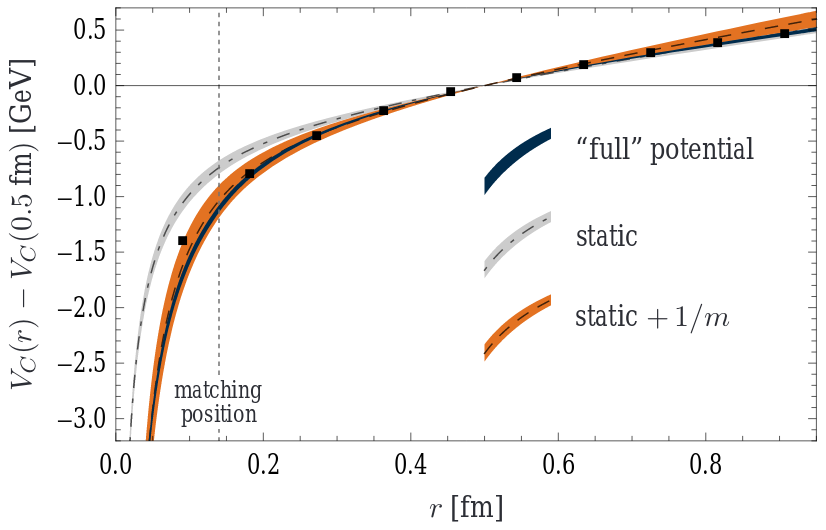
\includegraphics{ccbar_potential.png}
  \caption{Charmonium ($c\bar{c}$) potential from a combination of perturbative QCD (small $r$) and lattice QCD (large $r$) \cite{Laschka:2011zr}.}
  \label{fig:charmonium_potential}
\end{figure}

The heavy quark-antiquark potential can be computed with \ac{pQCD} at small separations and on the lattice for large separations, as shown in \cref{fig:charmonium_potential}.
The charmonium lattice \qcd potential with three light quarks and charm-quark mass effects is well-described to the 4-loop level by the parameterization \cite{Laschka:2011zr}
\begin{equation}
V_{c\bar{c}}(r) = - \frac{A}{r} + \sigma r
\end{equation}
with $A = 160 \pm 4 \MeV\,\fm$ and $\sigma = 790 \pm 30 \MeV/\fm$ (\cref{fig:charmonium_potential}).
The first term has the same form as an attractive Coulomb potential, albeit with a coupling constant about 2 orders of magnitude larger than the \ac{EM} coupling\footnote{where $\alpha_\textrm{EM} \hbar c \approx 1.44 \MeV\,\fm$}.
The latter term resembles the potential from the force by a string of constant tension $\sigma$, which invokes a description by color ``flux tubes'' between the two quarks of constant energy per length.
This ``string'' term increases without bound at large separations, so a quark-antiquark pair cannot be separated with a finite amount of energy.
At some point it becomes more energetically favorable to produce a quark-antiquark pair out of the vacuum than to maintain a long flux tube (\cref{fig:qqbar_flux}).
This property is responsible for the phenomenon of \emph{confinement}, which is the absence in nature of bare color charges.

\begin{figure}[t]
  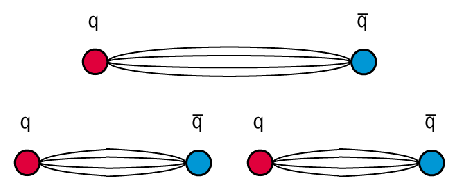
\includegraphics{qqbar_flux.png}
  \caption{The color flux tube between a quark-antiquark pair and the breaking of the flux tube into a new $q\bar{q}$ pair from the vacuum.}
  \label{fig:qqbar_flux}
\end{figure}

%% \todo{possibly add detail on lattice gauge theory}

\section{QCD at high temperatures}

Given the observed properties of asymptotic freedom and color confinement, a natural question is whether nuclear matter has a phase transition at large density and/or temperature.
In a system with a low number of quarks, the color connection keeps each bound tightly to others.
At high densities, however, individual flux tubes are not discernible, and individual color charges are easily balanced by nearby color sources.
Such a state could exhibit deconfinement, with color charge free to move as electric charge does in a conventional plasma.
This \qgp is expected to have different properties than hadronic matter.

\begin{figure}[t]
  %% https://homepages.uni-regensburg.de/~sow28704/ftd_lqcd_ss2012/ftd_lqcd_ss2012.html
  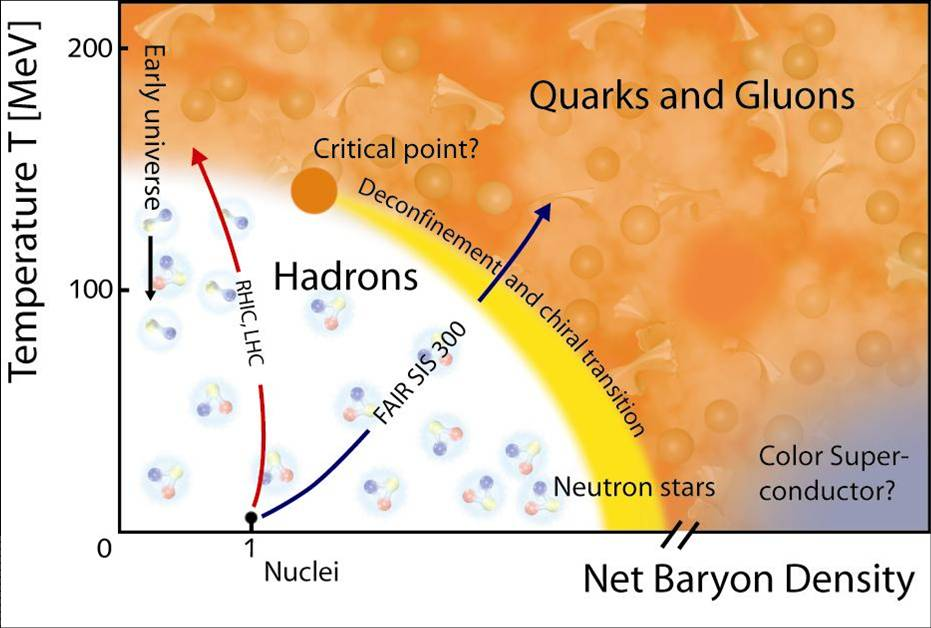
\includegraphics{qcd_phase.jpg}
  \caption{A conjectured phase diagram for QCD matter. The transition from hadronic matter to QGP at low baryon density is a smooth crossover. A critical point is hypothesized but not established.}
  \label{fig:qcd_phase}
\end{figure}

Dimensional analysis suggests that the critical temperature $T_c$ (at zero chemical potential) should be close to the only possibly relevant scale
\[
T_c \sim \lqcd \sim 10^{12}~\mathrm{K}\; .
\]
\cref{fig:qcd_phase} shows a conjectured phase diagram for \qcd matter.
The transition between hadronic matter and the QGP is a smooth crossover at low baryon density \cite{Aoki:2006we}.
Above some critical baryon density the transition is hypothesized to be first-order based on a number of model approaches, but this has not been established.

\subsection{Thermodynamics of relativistic systems}
For massless particles the probability of having energy $E$ is calculated by integrating over the constrained phase volume \( \frac{d^3 x \, d^3 p}{(2\pi)^3} \delta\left( E - |\mathbf{p}|\right)\) times the density of states.
With the statistical factor $\eta=\pm1$ for bosons/fermions and $\eta=0$ for non-identical particles, this gives a probability per unit volume of
\begin{equation}
\frac{g E^2}{2\pi^2} \frac{1}{e^{E/T} - \eta}
\end{equation}
where $g$ is a degeneracy factor e.g. for multiple spin values.
For non-identical particles this yields expressions for the energy and number density
\begin{align}
  \varepsilon_\textrm{NI} =& g\frac{3T^4}{\pi^2} \\
  n_\textrm{NI} =& g\frac{T^3}{\pi^2}
\end{align}
with
\begin{align}
  \varepsilon_\textrm{BE} =& g\frac{\pi^2 T^4}{30} \\
  n_\textrm{BE} =& g\frac{\zeta(3) T^3}{\pi^2}
\end{align}
for bosons and
\begin{align}
  \varepsilon_\textrm{FD} =& g\frac{7 \pi^2 T^4}{240} = \frac{7}{8} \varepsilon_\textrm{BE} \\
  n_\textrm{FD} =& g\frac{3 \zeta(3) T^3}{4 \pi^2} = \frac{3}{4} n_\textrm{BE}
\end{align}
for fermions.
Quantum statistical effects increase the energy and number density for bosons and decrease them for fermions so $\varepsilon_\textrm{FD} < \varepsilon_\textrm{NI} < \varepsilon_\textrm{BE}$.

For a non-interacting mixture the total energy density is
\begin{equation}
\varepsilon = \left( g_\textrm{BE} + \frac{7}{8} g_\textrm{FD} \right) \frac{\pi^2 T^4}{30}
\end{equation}
where the $g$ terms are the total degeneracy factors for relevant particle species.
For instance, at low temperatures where a system is hadron gas the degrees of freedom are the pions with 3 isospin possibilities, so $g_\textrm{BE} = 3$ and $g_\textrm{FD} = 0$.
In \qcd the energy density becomes\footnote{Gluons have $3^2 - 1 = 8$ possible colors and 2 possible spins, while each flavor of quark has 3 possible colors and 4 spinor components.}
\begin{equation}
  \label{eq:qcd_energy}
\varepsilon = \left( 32 + 21 N_f \right) \frac{\pi^2 T^4}{60}
\end{equation}
for $N_f$ active quark flavors at the temperature scale.
At a phase transition where the active thermodynamic degrees of freedom become quarks and gluons from pions the ratio $\varepsilon/T^4$ would be expected to increase by an order of magnitude.

\subsection{Thermal quantum field theory}
The probability of a thermal system to be in state $\psi$ is proportional to $e^{-\beta \hat{H}(\psi)}$ where $\beta = 1/T$ is the coldness and $H$ is the Hamiltonian of the configuration.
This is generally expressed in terms of the partition function
\begin{equation}
  \label{eq:z_classical}
Z(\beta) = \mathrm{tr} \left( e^{-\beta H} \right)
\end{equation}
so that the thermodynamic expectation value of an operator $\mathcal{O}$ is given by
\begin{equation}
\langle \mathcal{O} \rangle = \frac{1}{Z} \mathrm{tr} \left( \mathcal{O} e^{-\beta H} \right) \;.
\end{equation}
In \ac{QFT} the partition function is represented by the path integral
\begin{equation}
  \label{eq:z_qft}
  Z = \int \mathcal{D}[\psi] \, e^{i\int d^4 x \, \Lagr(\psi)}
\end{equation}
from which amplitudes can be calculated through functional derivatives of source terms $J \cdot \psi$ in the Lagrangian density.
At the same time, by analogy with \cref{eq:z_classical} the thermal partition function must look something like
\begin{equation}
  \label{eq:z_analogy}
Z \sim \int \mathcal{D}[\psi] \, e^{-\beta \int d^3 \mathbf{x} \, \mathcal{H}(\psi)}
\end{equation}
in terms of the Hamiltonian density $\mathcal{H}$.
The Lagrangian can be related to the Hamiltonian by a Wick rotation $t \rightarrow -i\tau$ which transforms $\mathcal{L} \rightarrow - \mathcal{H}$.
With the transformation of the temporal integral in the exponent $i \int dt$ into a periodic domain $\int_0^\beta d\tau$ this analogy can be made precise.
The fields are periodic such that \(\psi(\beta,\mathbf{x}) = \pm \psi(\beta,\mathbf{x})\) where the sign is determined by whether the field is a boson or fermion.
This periodicity leads to discretization of the allowed energies where $E_n = 2n\pi T$ for bosons and $E_n = (2n+1)\pi T$ for fermions.

With this formalism the full power of perturbation theory can be applied to calculate a number of observables \cite{Gross:1980br}.
The real-time tree-level propagators pick up absorptive terms proportional to \(2\pi \delta(p^2 - m^2) \frac{1}{e^{\beta |p^0|} \mp 1} \) for bosons/fermions.
For instance, computation of the free energy $ -T \log Z$ leads to a corresponding \ac{LO} correction to \cref{eq:qcd_energy}.
\begin{equation}
  \label{eq:qcd_energy_lo}
\frac{\varepsilon}{T^4} = \left( \frac{4\pi}{15} - \alpha_s \right)2\pi + \left(\frac{7\pi}{10} - \frac{5}{3}\alpha_s \right)\frac{\pi N_f}{2}
\end{equation}


\subsection{Equation of state from lattice calculations}
\label{subsec:lattice}

\begin{figure}[t]
  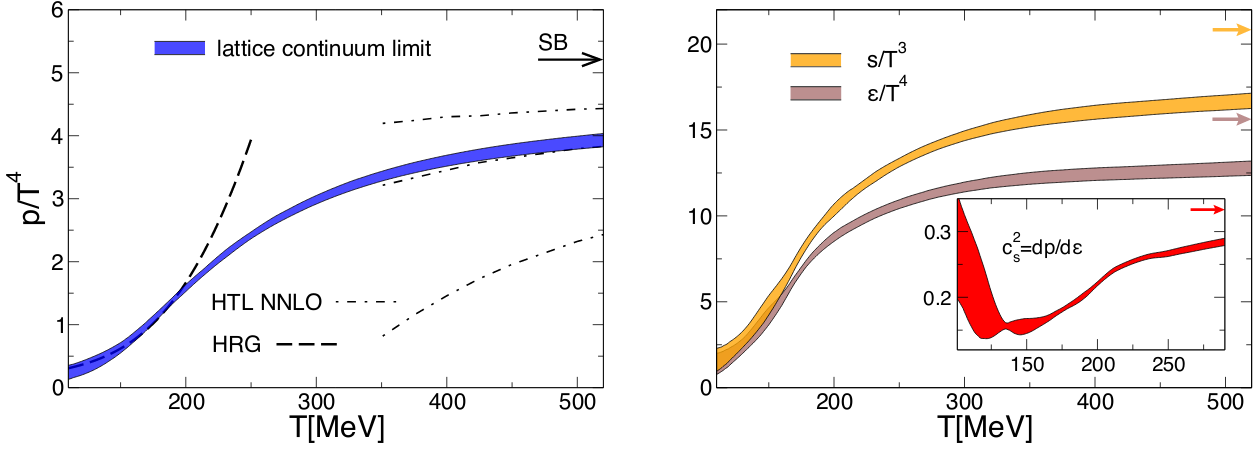
\includegraphics[width=\linewidth]{lattice_eos.png}
  \caption{The trace anomaly for several values of lattice spacing $N_\tau = 1/aT$ and the continuum extrapolation (left), and thermodynamic quantities in the continuum limit (right), both shown as a function of temperature \cite{Bazavov:2014pvz}. The solid lines show the predictions from the HRG model, and the Stefan-Boltzmann limit for 3 quark flavors at $19\pi^2/12$ is shown by the straight dashed line.}
  \label{fig:lattice_eos}
\end{figure}

%% the latter HotQCD ref is slightly more recent and has many good plots including static potential (no 1/m corrections?)
Thermodynamic quantities can be computed in lattice \qcd at small chemical potential \cite{Borsanyi:2013bia,Bazavov:2014pvz}.
The results are clearly distinct from the \ac{HRG} model \cite{Huovinen:2009yb}, indicating that deconfinement is a fundamental property of the transition.
The trace anomaly $T_\mu^\mu = \varepsilon - 3 p$, where $\varepsilon$ is the energy density and $p$ is the pressure, is computed in lattice calculations as a function of temperature.
It vanishes in a conformal theory, so the appearance of a significant trace anomaly with a peak around $200 \MeV$ suggests the emergence of a scale dependence.
The pressure is related to the derivative of the trace anomaly up to factors of the temperature.
From there, the remaining combinations of thermodynamic quantities such as $\varepsilon(T)$ and the entropy density $s = \frac{\varepsilon + p}{T}$ are computed, determining the \ac{EoS}.

Recent lattice \qcd results are shown in \cref{fig:lattice_eos}.
The large step in the ratios $\varepsilon/T^4$ and $s/T^3$ around the critical temperature is an indication of a phase transition indicated by the increase in the effective number of degrees of freedom in \qcd matter.
A smooth crossover is observed with a critical temperature of \( T_c = 170 \pm 4 \MeV \) \cite{Aoki:2009sc}, which is indeed close to \lqcd as predicted by dimensional analysis.
Above the critical temperature, clear deviations are shown from the predictions of the \ac{HRG} model.
The Stefan-Boltzmann limit does not appear to be reached.
This appears to be consistent with \cref{eq:qcd_energy_lo} which says that perturbative corrections to the energy are negative.


\subsection{Heavy ion collisions}

Heavy ions like gold-197 and lead-208 have hundreds of nucleons packed into a spherical volume of radius $\sqrt[3]{A} \approx 6$ times that of a proton.
This also corresponds to an average transverse areal density of the same factor of 6 times larger than that of a proton.
In a head-on \AuAu or \PbPb collision, roughly 200 times the energy interacts in a transverse area about 35 times larger than a \pp collisions of the same $\sqrt{s_\mathrm{NN}}$.
Hydrodynamic modeling suggests a formation time on the order of 1 fm/c, so na\"ively the ultra-relativistic initial products of nuclear collisions have the potential to reach thermalization in \AA collisions.

%% \subsubsection{Glauber model} %% don't really need an extra subsection label?
\begin{figure}[t]
  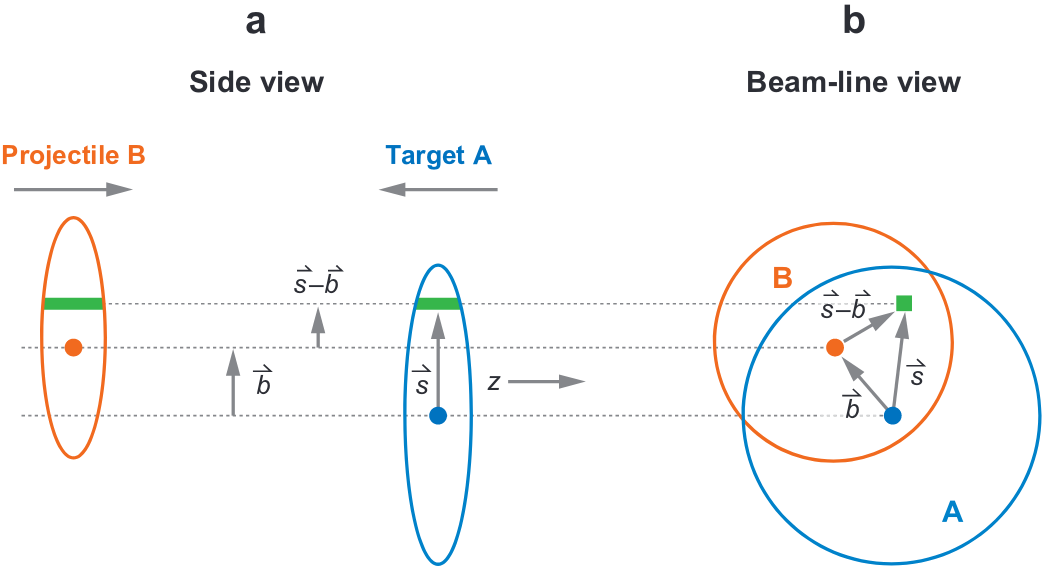
\includegraphics{hi_collision_geo.png}
  \caption{Diagram of the Glauber model nucleus-nucleus geometry with transverse (a) and longitudinal (b) perspectives \cite{Miller:2007ri}.}
  \label{fig:hi_collision_geo}
\end{figure}

The size and shape of the energy density deposited in a heavy ion collision varies greatly depending on the impact parameter $b$, as illustrated in \cref{fig:hi_collision_geo}.
The Glauber model is used to describe the average energy density in nuclear collisions as a function of impact parameter \cite{Miller:2007ri}.
In the optical limit of smooth density, the nuclear density $\rho$ is parameterized by the Woods-Saxon distribution
\begin{equation}
\rho(r) = \frac{\rho_0}{1 + \exp\left( \frac{r-R}{a} \right)} \, ,
\end{equation}
where $R$ and $a$ are the radius and skin depth of the nucleus, respectively.
The normalization constant \[\rho_0 = \frac{3A}{4 \pi R^3} \left[1 + \frac{\pi^2 a^2}{R^2}  + \bigo{e^{-R/a}}\right]^{-1}\] is set to fix the integral to the total number of nucleons\footnote{The exact expression in terms of the trilogarithm function is \( \rho_0 = \frac{A}{-8\pi a^3 \mathrm{Li}_3\left( -e^{R/a} \right)} \).}.
The radial density distribution for lead-208 is shown in \cref{fig:woods_saxon}, with $R = 6.62 \pm 0.06~\fm$ and $a = 0.55 \pm 0.01~\fm$.

\begin{figure}[t]
  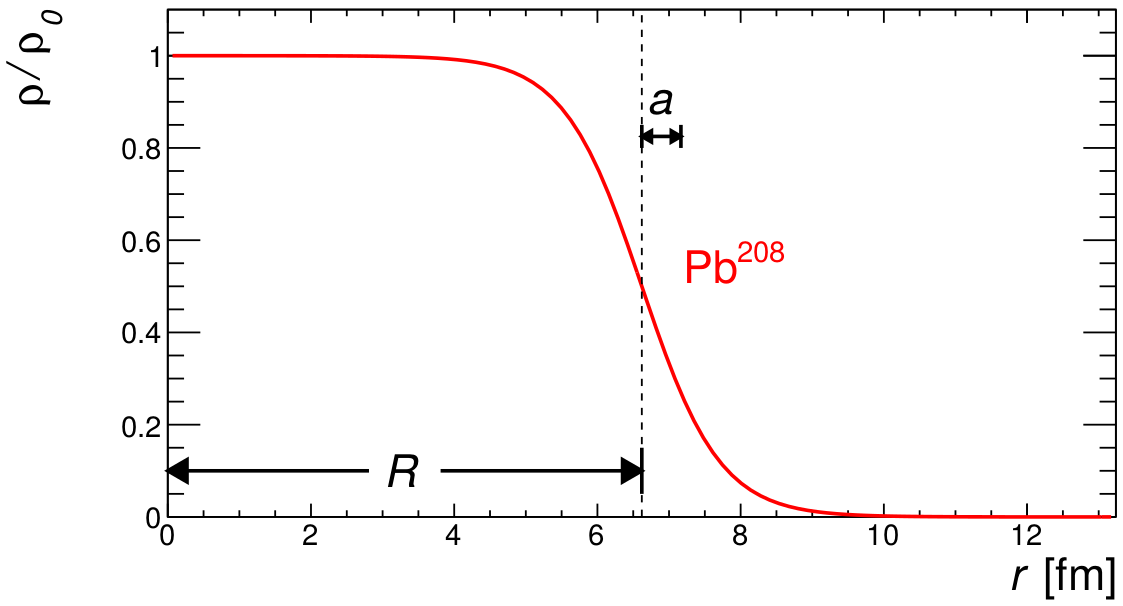
\includegraphics{woods_saxon_pb208.png}
  \caption{The density as a function of radius following the Woods-Saxon distribution for the ${}^{208}\mathrm{Pb}$ nucleus.}
  \label{fig:woods_saxon}
\end{figure}

The transverse density of a nucleus with mass number $A$ at a transverse position $\mathbf{s}$ relative to its center is given by the projection of the spherical density along a longitudinal axis.
\begin{equation}
T_A(\mathbf{s}) = \int dz \, \rho_A\left( \sqrt{s^2 + z^2} \right)
\end{equation}
For two nuclei with mass numbers $A$ and $B$ colliding with impact parameter $\mathbf{b}$, the thickness function is
\begin{equation}
T_{AB}(\mathbf{b}) = \int d^2 b \, T_A(\mathbf{s}) T_B(\mathbf{s} - \mathbf{b}) \;,
\end{equation}
which has units of inverse area.
The expected number of nucleon-nucleon collisions \Ncoll is obtained by multiplying the thickness function by the inelastic nucleon-nucleon cross-section\footnote{More rigorously, the probability distribution of \Ncoll for a given impact parameter $b$ is the binomial distribution with $n = AB$ and $p = \frac{T_{AB}(b) \sigma^{NN}_\mathrm{inel}}{AB}$. }
\begin{equation}
  \langle\Ncoll(b)\rangle = T_{AB}(b) \sigma^{NN}_\mathrm{inel} \;.
\end{equation}
%% The inelastic nucleus-nucleus cross-section is
%% \begin{equation}
%% \frac{d^2 \sigma^{AB}_\mathrm{inel}}{db^2} = 1 - \left[ 1 - \frac{T_{AB}(b) \sigma^{NN}_\mathrm{inel}}{AB} \right]^{AB} \;.
%% \end{equation}
The number of nucleons in both target and projectile that interact is called the number of participating nucleons, \Npart, or the number of wounded nucleons.
\begin{equation}
  \begin{split}
  \langle \Npart(b) \rangle = &\int d^2 s \, T_A(\mathbf{s})\left\{ 1 - \left[ 1 - \frac{T_B (\mathbf{s} - \mathbf{b}) \sigma^{NN}_\mathrm{inel}}{B} \right]^B \right\} + \\
  &\int d^2 s \, T_B(\mathbf{s}-\mathbf{b})\left\{ 1 - \left[ 1 - \frac{T_A (\mathbf{s}) \sigma^{NN}_\mathrm{inel}}{A} \right]^A \right\}
  \end{split}
\end{equation}

The optical approximation taken here is not able to account for fluctuations in nucleon positions within the nuclei.
To remedy this, a \mc approach can be taken which randomizes the impact parameter according to $P(b) \propto 2\pi b$ and the positions of the nucleons within each nucleus according to the Woods-Saxon distribution.
One method is to tag a nucleon as wounded if its distance in the transverse plane is within $\sqrt{\sigma^{NN}_\mathrm{inel}/\pi}$ of any nucleon in the other nucleus.
The expectation values of \Ncoll and \Npart can be calculated as a function of $b$ by repeated simulations. 
The Glauber \mc model predicts some shadowing of the total nucleus-nucleus cross-section relative to the optical approach, but differences in the expected \Ncoll and \Npart are negligible \cite{Miller:2007ri}. %% todo: show figure 5 from this reference here? probably not

In experiments the impact parameter cannot be measured directly so a proxy must be used.
This is typically the charged-particle multiplicity or the total energy deposited at large $|\eta|$.
Because there is a probabilistic component to the particle production at a given $b$, results are often reported in intervals of event activity, either in percentile or the corresponding expected \Npart.

\subsection{Proton-nucleus collisions}
The initial motivation for studying proton-nucleus collisions is to understand \ac{CNM} effects.
Measurements from \AA collisions are often normalized by the same quantities in \pp collisions up to factors of \Npart.
Heavy ion collisions are not completely equivalent to a sum of several \pp collisions, due in part to the presence of additional spectator nucleons.
Proton-nucleus collisions can be used to control for these effects.
The physics of \pA collisions has also turned out to be surprisingly interesting in its own right.

In \pA collisions the expected number of collisions is given in terms of the single-nucleon thickness function
\begin{equation}
  \langle \Ncoll(b) \rangle = T_A(b) \sigma^{NN}_\mathrm{inel}
\end{equation}
and the number of nucleon participants is simply
\begin{equation}
  \Npart = \Ncoll + 1 \;.
\end{equation}
Because the projectile consists of a single proton, event-by-event fluctuations in its size can impact the \Npart significantly.
In \AA collisions the effect of such fluctuations is washed out because the relative fluctuations in the projectile cross-section are suppressed by a factor of $A^{-1/2}$.
The \ac{GGCF} model provides the framework to describe this effect by parameterizing fluctuations in $\sigma^{NN}_\mathrm{inel}$ with the dimensionless parameter $\omega_\sigma$.
The \Npart distribution is shown in \cref{fig:ggcf_npart} for the Glauber model and two values of the \ac{GGCF} extension.
Fluctuations in $\sigma^{NN}_\mathrm{inel}$ put higher weight into the high-\Npart tail of the distribution.

\begin{figure}[t]
  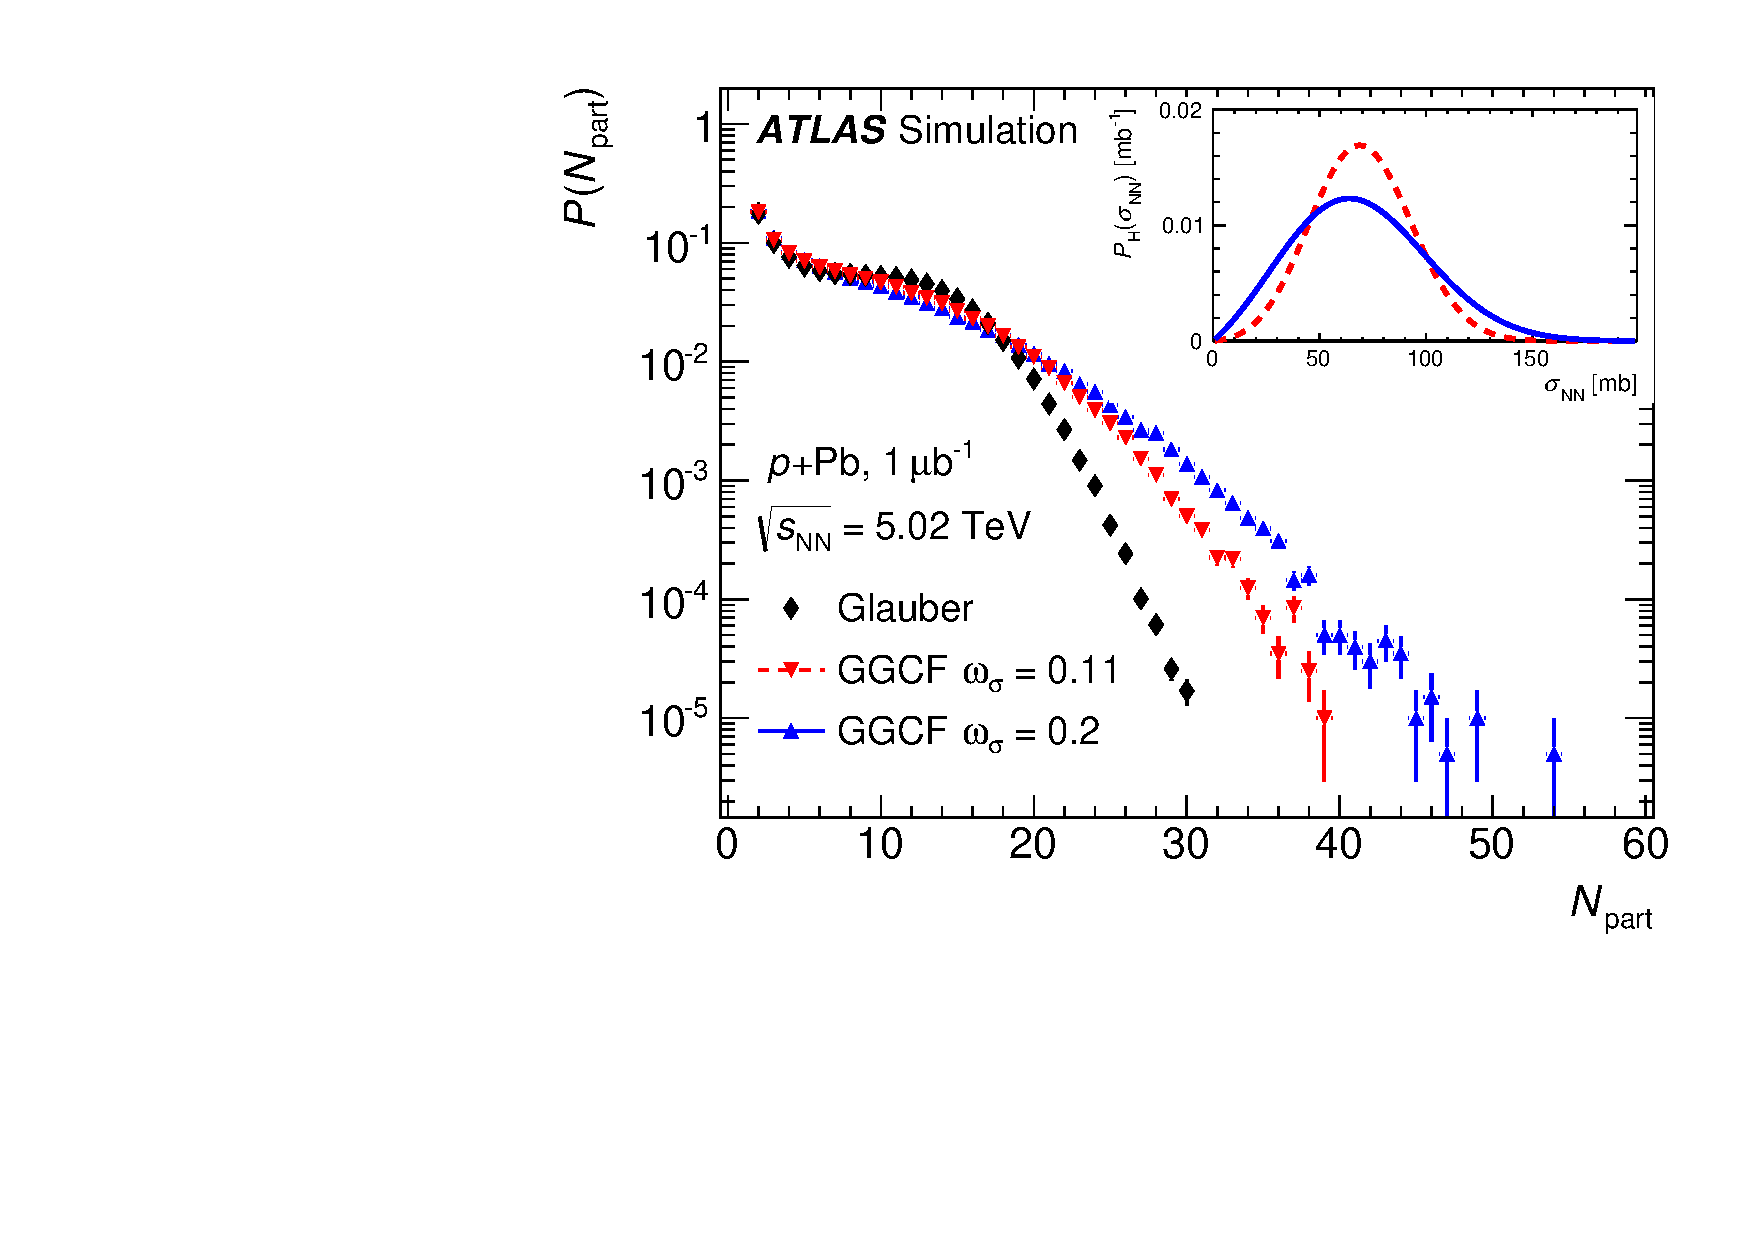
\includegraphics[width=0.49\linewidth]{ggcf_prob_dist.pdf}
  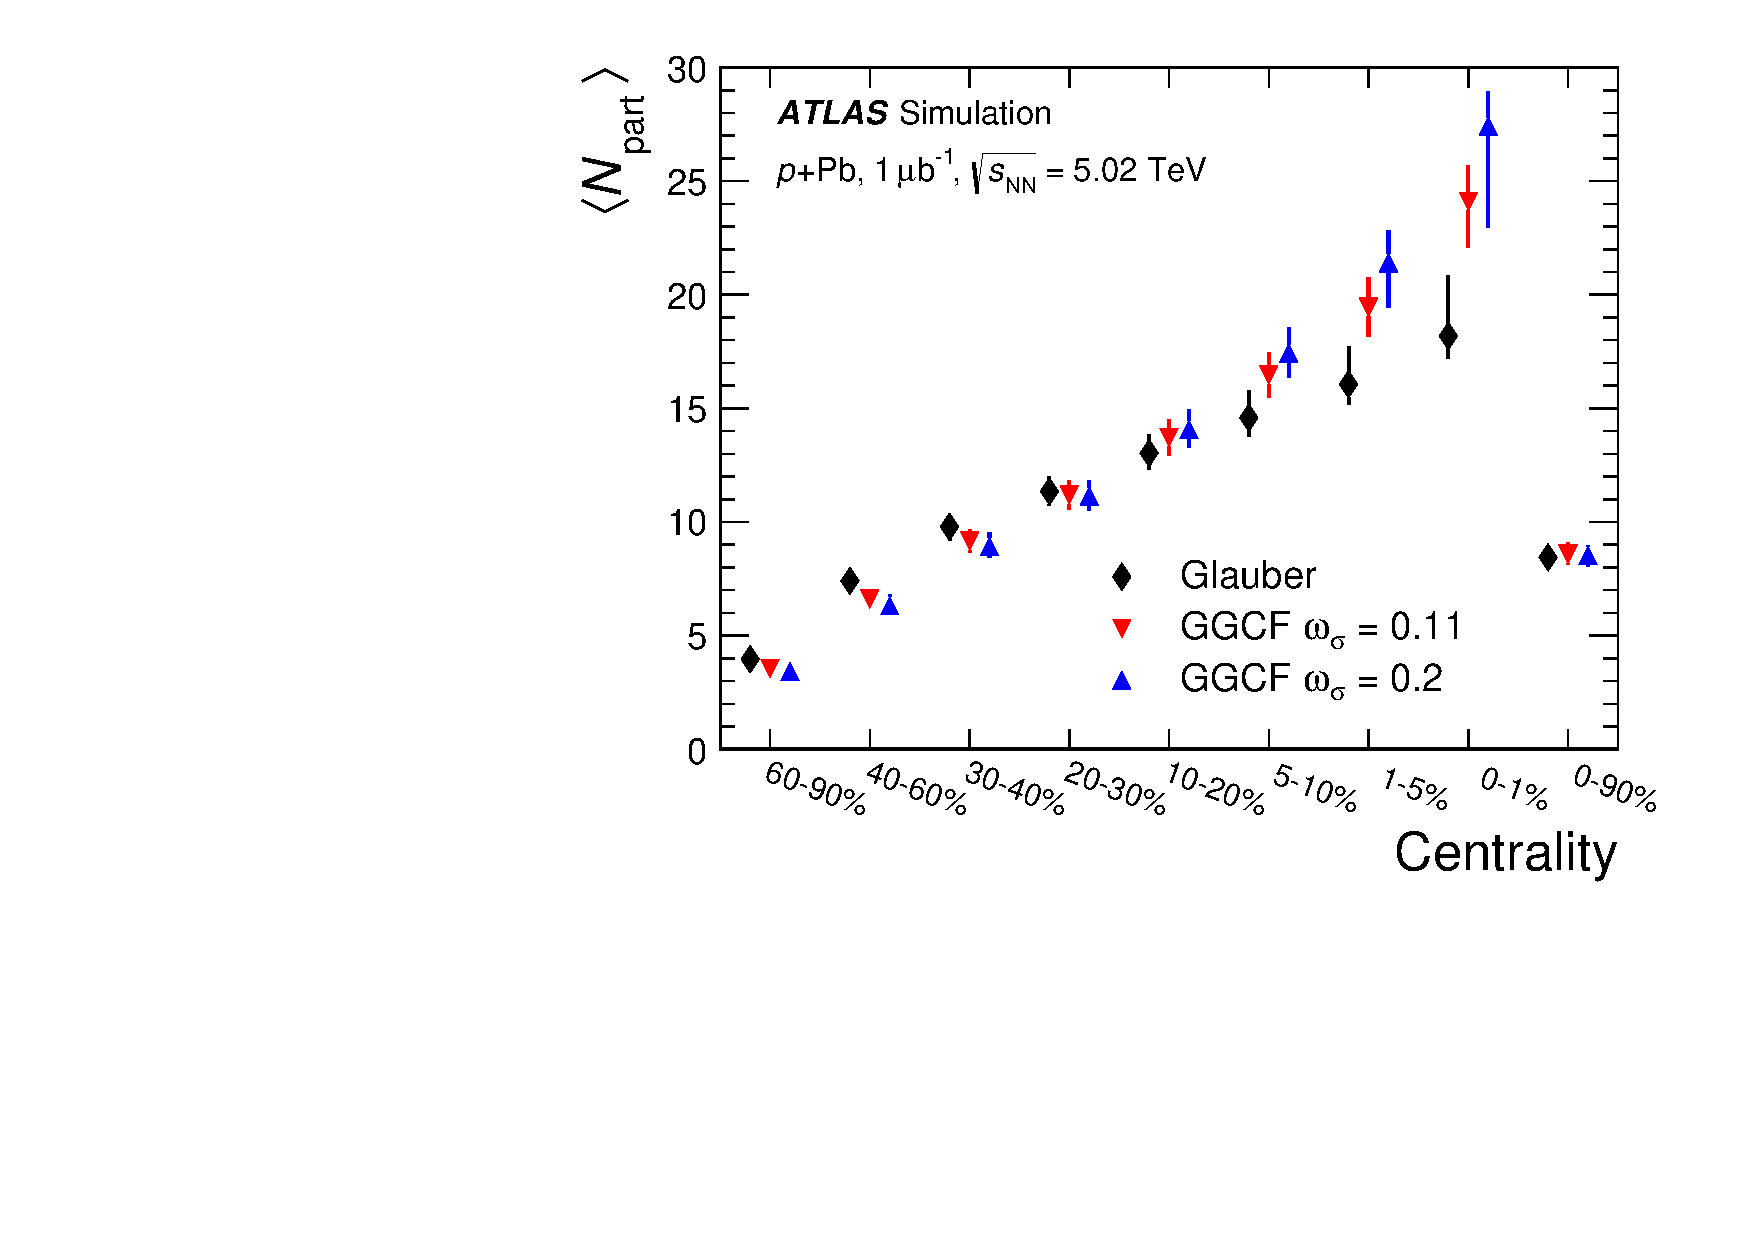
\includegraphics[width=0.49\linewidth]{npart_ggcf.pdf}
  \caption{The \Npart distribution for proton-lead collisions using the Glauber model and the generalized color fluctuation model (left), along with the \avgNpart for the corresponding centrality intervals with each model (right) \cite{HION-2012-15}.}
  \label{fig:ggcf_npart}
\end{figure}

Measurements of charged particle multiplicity and $Z$ boson production suggest that the geometry is best described by $\omega_\sigma > 0$ \cite{HION-2012-15,HION-2013-09}.
The precise value is not well-constrained but a value of $\omega_\sigma = 0.11$ is slightly preferred over the higher value of $0.2$.
Results presented in this thesis will provide additional support for the \ac{GGCF} model with $\omega_\sigma > 0$.


\subsection{Experimental status of the strongly-coupled QGP}

\subsubsection{Hard sector}

\begin{figure}[t]
  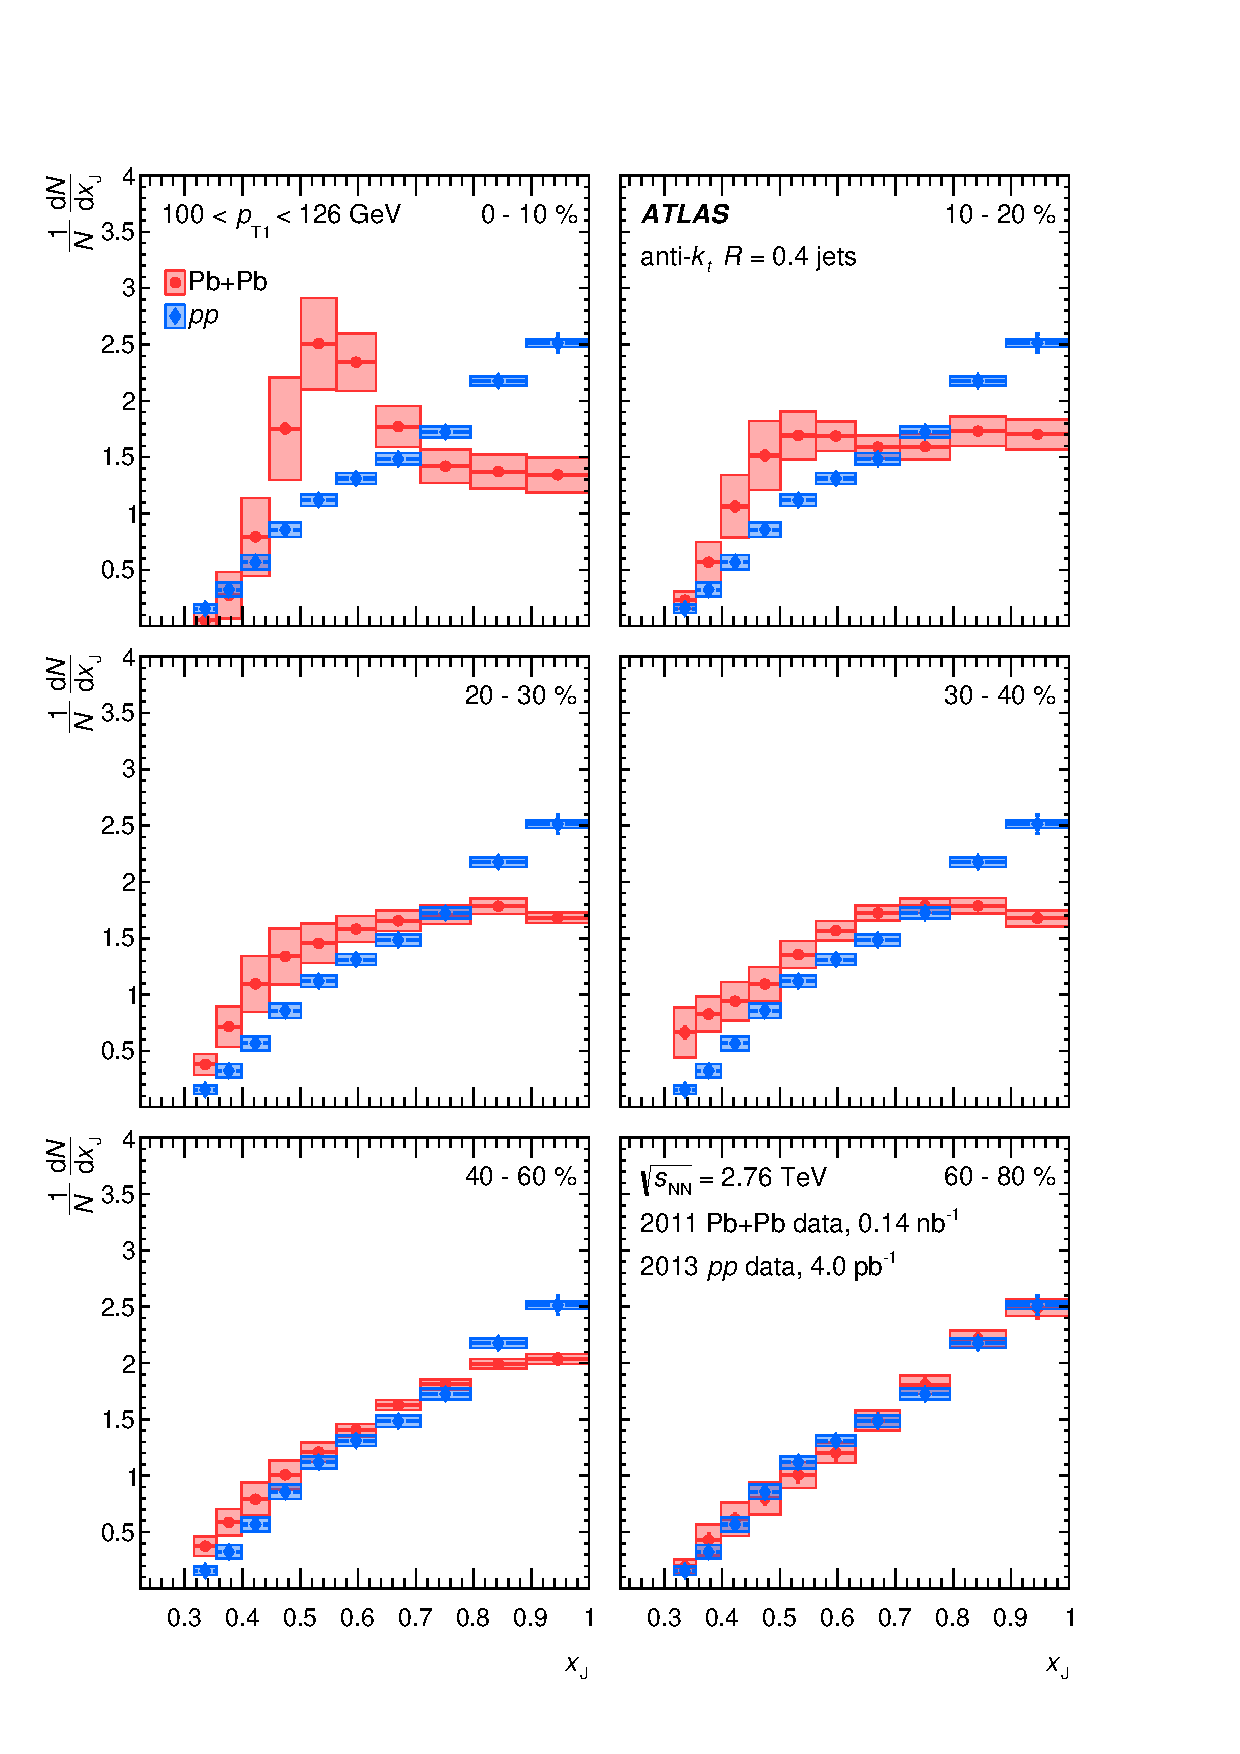
\includegraphics{dijet_asym.pdf}
  \caption{The distribution of the sub-leading jet suppression $x_\textrm{J}$ as a function of centrality in lead-lead collisions \cite{HION-2012-11}. The observable $x_\textrm{J}$ is defined as the ratio of sub-leading to leading jet \pt and is reduced relative to proton-proton collisions. The distributions are unfolded to correct for detector resolution effects.}
  \label{fig:dijet_asym}
\end{figure}

The observation of jet quenching in \PbPb collisions, shown in \cref{fig:dijet_asym}, is a signature of the formation of an opaque medium \cite{HION-2012-11}.
The reduction of the ratio of sub-leading jet \pt to leading jet \pt is drastic in central collisions but not significant in peripheral collisions.
This matter is likely composed of relatively soft particles since if the suppression was a result of hard scattering alone dijets would be deflected at large angles.
Dijet asymmetry has not been observed in \pA collisions, but this does not necessarily rule out the formation of a medium because it could have a formation time comparable to the transverse size of the system.

\begin{figure}[t]
  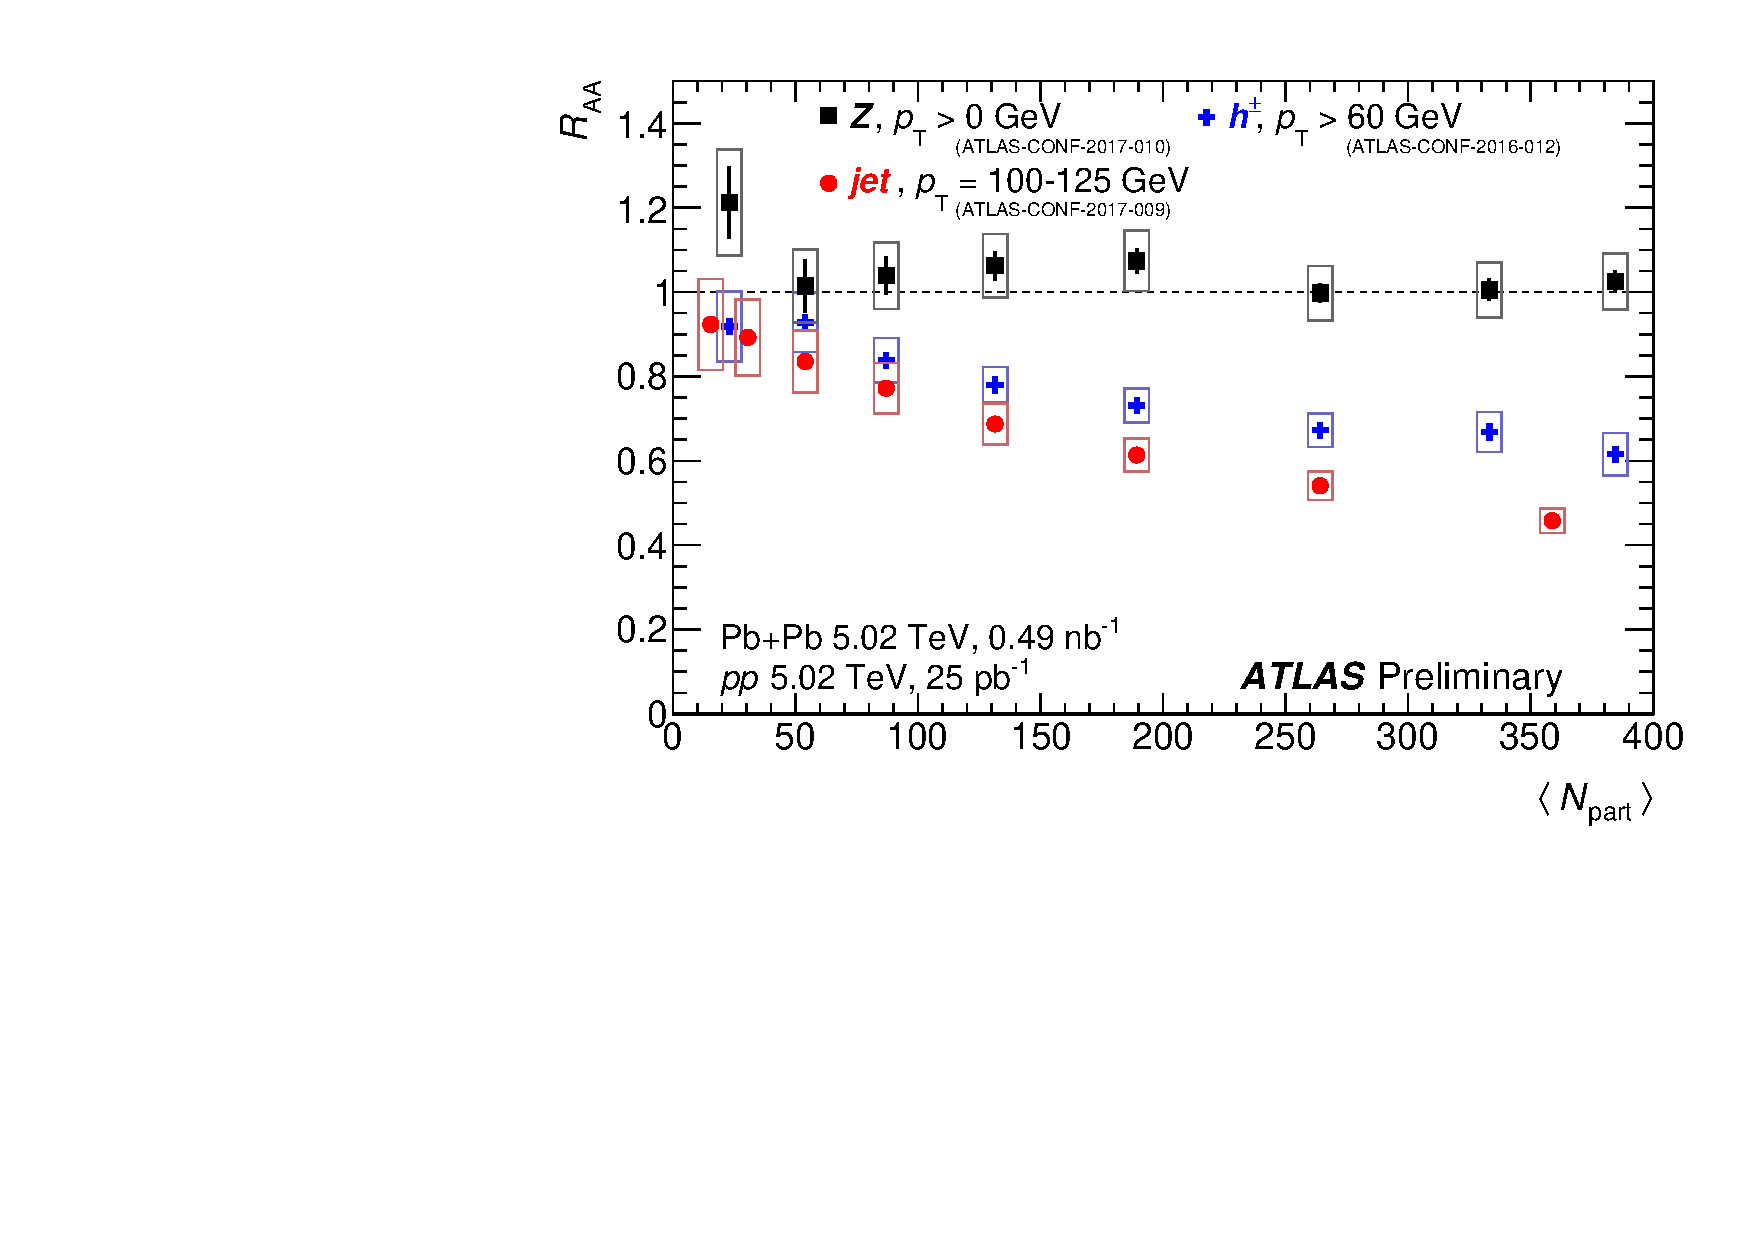
\includegraphics{ATLAS_HION_Summary_Raa_02.pdf}
  \caption{Summary of the nuclear modification factor \RAA for a few relevant production channels in lead-lead collisions. No suppression is observed for the colorless $Z$ bosons, but high-\pt jets and hadrons are suppressed with an increased effect in central collisions.}
  \label{fig:pbpb_raa}
\end{figure}

Jet and particle production in heavy ion collisions is often reported in terms of the nuclear modification factor \RAA of channel $X$.
\begin{equation}
  \RAA = \frac{\frac{1}{\Nevt}\frac{d N^{AA}_{X}}{d^3 p}}{\langle T_{AA} \rangle \frac{d\sigma^{pp}}{d^3 p}}
\end{equation}
An $\RAA < 1$ is called \emph{suppression}, and is often interpreted as absorption or slowing of the channel in question.
As shown in \cref{fig:pbpb_raa}, high-\pt hadrons and jets are suppressed in \PbPb collisions which suggests that they interact with a medium.
This suppression is stronger in central collisions where a greater mass and volume of medium is produced \cite{HION-2013-06}.
The \RAA for $Z$ bosons is shown as a control measurement because electoweak bosons do not interact via the color force and thus are expected to pass through any \qgp.

\begin{figure}[t]
  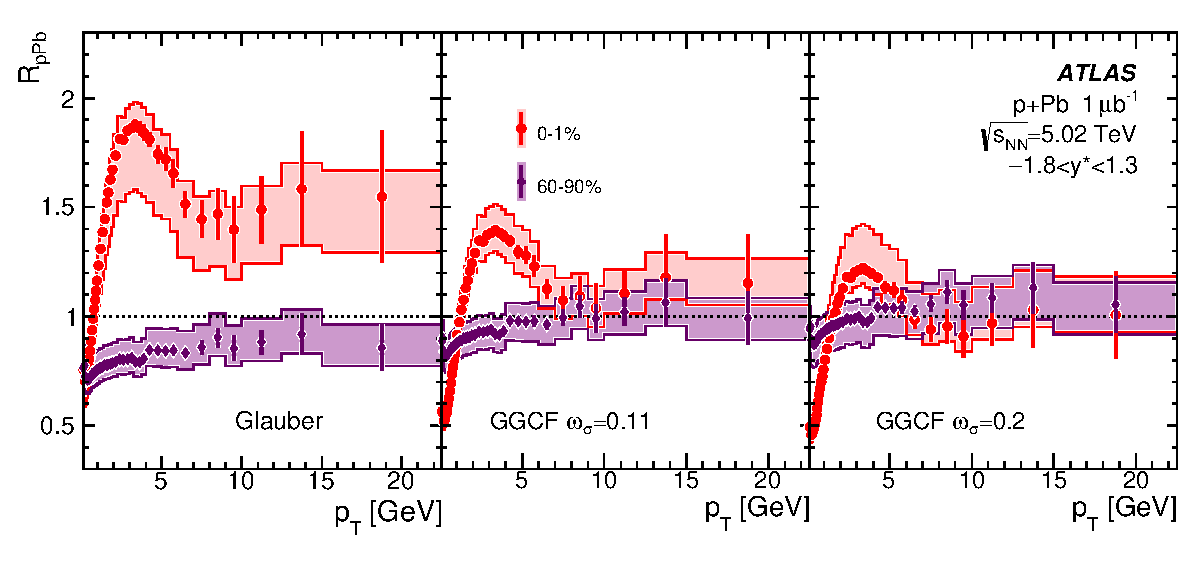
\includegraphics{rppb_cp.pdf}
  \caption{\RpPb for charged particles as a function of \pt for different collision geometries in the Glauber-Gribov color fluctuation model \cite{HION-2012-14}.}
  \label{fig:rppb_cp}
\end{figure}

A similar ratio is defined for \pA collisions.
\begin{equation}
  \RpA = \frac{\frac{1}{\Nevt}\frac{d N^{pA}_{X}}{d^3 p}}{\langle T_{pA} \rangle \frac{d\sigma^{pp}}{d^3 p}}
\end{equation}
For charged particles an apparent enhancement at high \pt can be explained by the \ac{GGCF} model \cite{HION-2012-14}, as shown in \cref{fig:rppb_cp}.
There is a sign of rapidity-dependent jet suppression in central \pPb collisions \cite{HION-2013-08}, although this is not a smoking gun for any medium formation because \RpPb is sensitive to other production effects like modifications to the nuclear \ac{PDF}.


\FloatBarrier
\subsubsection{Soft sector}

Particle production in high energy collisions is often decomposed into azimuthal Fourier components \cite{Voloshin:1994mz,Poskanzer:1998yz}. %% Heinz:2013th more recent summary
\begin{equation}
  \label{eq:flow_coefficients}
  E \frac{d^3 N}{d^3 p} = \frac{1}{2\pi \pt} \frac{d^2 N}{d\pt \, dy}\left\{ 1 + \sum_{n=1}^{\infty} 2v_n \cos\left[n(\phi - \Psi_n) \right] \right\}
\end{equation}
The $v_n$ are called the $n$th-order flow coefficients and the $\Psi_n$ are the $n$th-order event plane.
Experimentally they are defined by the relation (without corrections)
\begin{equation}
v_n e^{in\Psi_n} = \sum_k w_k e^{in\phi_k}
\end{equation}
where $w_k$ weights the $k$th particle or calorimeter element and is typically the \pt or $E_\mathrm{T}$ of the component.
This provides a framework for testing the predictions of dynamical models that describe the evolution of the initial energy deposited in the collision to the final-state bulk of particles.
For instance, a non-interacting gas model predicts $\langle v_n \rangle = 0$ for $n \geq 2$, with nonzero flow coefficients only from fluctuations, and is ruled out for \AA, \pA, and \pp collisions.

Hydrodynamics is a simple model that only assumes the system can be described by a fluid field with four-velocity $u^\mu(x^\nu)$ and imposes conservation of the stress-energy tensor $T^{\mu\nu}$ and possibly other conserved charges. %%, such that $\nabla_\mu T^{\mu\nu} = 0$.
The inputs into hydrodynamics are the description of $T^{\mu\nu}$ itself, which typically includes an \ac{EoS} and multiple free parameters.
\Cref{sec:hydro} discusses relativistic hydrodynamic theory in detail.
The signature feature of fluid dynamics is the fact that accelerations are driven by pressure gradients.
For instance, in an ideal conformal fluid in $d$ spacetime dimensions
\begin{equation}
\dot{\mathbf{u}} = - \frac{1}{d} \boldsymbol{\nabla} \ln p
\end{equation}
where $\mathbf{u}$ is the vector part of $u^\mu$ and $p$ is the pressure.
Thus the shape of the initial energy density has a significant effect on the final particle distribution in \cref{eq:flow_coefficients}, as fluid is pushed from regions of large density to small.

For the fluid description to be valid, matter must be able to readily interact with nearby fluid.
If disturbances in the velocity and energy fields are not propagated to nearby locations then the smooth description of the fields breaks down.
This requires the mean free path \mfp to be small compared to the length scale that the system evolves over, or equivalently, that the viscosity is small.
The applicability of hydrodynamics is discussed in further detail in \cref{subsec:hydro_applicability}.

\begin{figure}[t]
  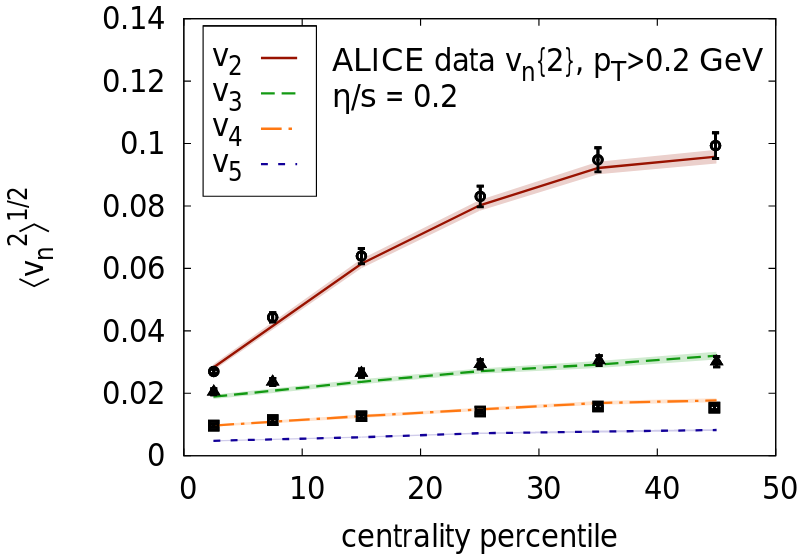
\includegraphics[width=0.49\linewidth]{vn_vs_cent.png}
  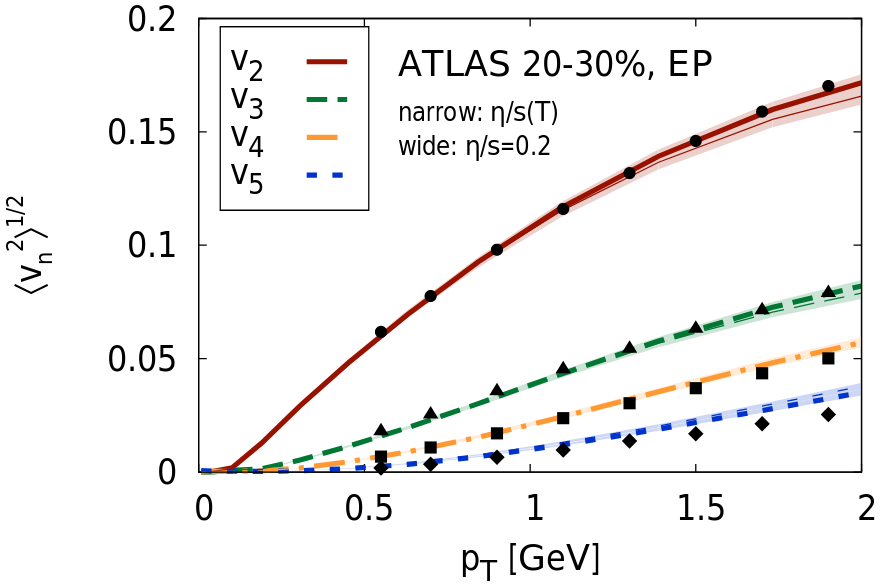
\includegraphics[width=0.49\linewidth]{vn_vs_pt.png}
  \caption{Event-by-event viscous hydrodynamic simulations of lead-lead collisions from \Ref{\cite{Gale:2012rq}} showing excellent agreement with experimental results as a function of centrality (left) \cite{ALICE:2011ab} and \pt (right) \cite{HION-2011-01}.}
  \label{fig:pbpb_vn}
\end{figure}

To a reasonable approximation, the 2nd- and 3rd-order flow coefficients are proportional to the corresponding eccentricities of the transverse source density \cite{Qiu:2011iv}, although $v_n$ for $n \geq 4$ include higher-order products.
The centrality of a \AA collision provides a control on the initial ellipticity, which is small for head-on central collisions with a circular transverse profile and larger for mid-central collisions with an almond-shaped overlap profile.
The $v_2$ as a function of centrality behaves according to this hydrodynamic prediction in \PbPb collisions.
Higher-order flow coefficients do not exhibit a strong centrality dependence because the higher-order eccentricities are not greatly dependent on the centrality.
The detailed simulations shown in \cref{fig:pbpb_vn} exhibit this behavior with excellent agreement with data as a function both of centrality and \pt.

Another key observation in \AuAu collisions is the scaling of the hadron flow coefficient with the hadron's number of constituent quarks $n_q$ \cite{Adare:2006ti}.
The hadron elliptic flow is found to scale with the kinetic energy such that $v_2^\textrm{hadron} = n_q v_2^\textrm{parton} \left(KT_\mathrm{T} / n_q\right)$.
This shows that the quarks themselves are indeed deconfined in the flow of the system, which amounts to strong evidence for the existence of the \qgp.

In \pp or \pA systems where the projectile has a radius that may be comparable to or smaller than the formation time, hydrodynamics is not na\"ively expected.
However, observations of a near-side azimuthal correlations in \pPb \cite{Abelev:2012ola,CMS-HIN-12-005,HION-2013-04} and \pp \cite{CMS-QCD-10-002,HION-2015-09} collisions show that these also exhibit collectivity, which is defined as pair correlations that arise not from direct interaction but from the global bulk evolution.
This ``ridge'' allows for the possibility of hydrodynamics in these smaller collisions, but hydrodynamics is not a necessary condition for collective behavior.
For instance, a \cgc model that invokes saturation of nuclear \acp{PDF} can predict a ridge in small systems with some success \cite{Dusling:2012cg,Dusling:2012wy,Dusling:2013qoz,McLerran:2013una,Kovchegov:2014yza}.

\begin{figure}[t]
  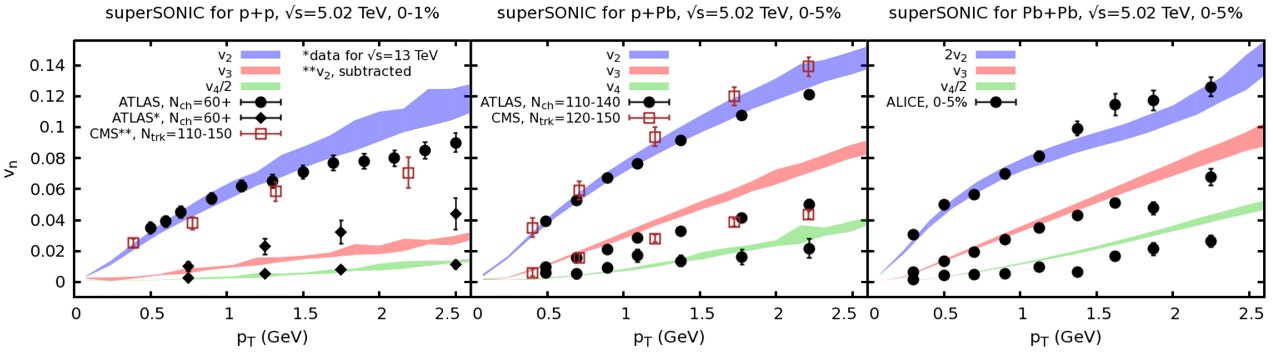
\includegraphics[width=\linewidth]{vn_all.png}
  \caption{Elliptic, triangular, and quadrupolar flow coefficients from superSONIC simulations (bands) compared to experimental data for proton-proton (left), proton-lead (center), and lead-lead (right) collisions \cite{Weller:2017tsr}. The specific viscosity parameters used in the simulations are $\eta/s = 0.08$ and $\zeta/s = 0.01$.}
  \label{fig:vn_all}
\end{figure}

Nevertheless, state-of-the-art viscous hydrodynamic simulations are capable of describing the flow coefficients in \pp, \pA, and \AA collisions simultaneously, as shown in \cref{fig:vn_all} \cite{Weller:2017tsr}.
Even in \pp collisions the $v_2$ seems to persist down to $\Nch \sim 20$ \cite{HION-2016-01}, however there is not yet complete agreement in the field over the experimental procedures used to extract the flow coefficients at very low \Nch.
For a review of hydrodynamics in small systems consult \Ref{\cite{Nagle:2018nvi}}.


\FloatBarrier
%% --------------------------------
%% Hydrodynamics
%% --------------------------------

\section{Hydrodynamic description of heavy ion collisions}
\label{sec:hydro}

\subsection{Relativistic fluid dynamics}

%% Poincar\'e instead of Lorentz?
Under the constraints of Lorentz symmetry and neglecting fluctuations, the stress-energy tensor of a perfect fluid described by flow four-velocity $u^\mu(x^\nu)$ is
\begin{equation}
%% T^{\mu\nu} = \left( \varepsilon + p \right) u^\mu u^\nu - p g^{\mu\nu} %% metric term has opposite sign for time-positive metric
T^{\mu\nu}_{(0)} = \varepsilon u^\mu u^\nu - p \Delta^{\mu\nu}
\end{equation}
where $\varepsilon$ and $p(\varepsilon)$ are respectively the energy density and pressure in the local rest frame.
The co-moving time-like and space-like projection operators are $u^\mu u^\nu$ and \( \Delta^{\mu\nu} \equiv g^{\mu\nu} - u^\mu u^\nu \) respectively.
In the absence of sources there are four conserved quantities corresponding to energy and three components of momentum.
\begin{equation}
  \label{eq:em_cons}
  \nabla_\mu T^{\mu\nu} = 0
\end{equation}
Projecting this equation into time and space components yields the relativistic Euler equations
\begin{align}
  D\varepsilon + \left(\varepsilon + p\right)\nabla^\perp_\mu u^\mu &= 0 \\
  \left(\varepsilon + p\right)Du^\mu + c_s^2 \nabla_\perp^\mu \varepsilon &= 0 
\end{align}
where \(D \equiv u^\mu \nabla_\mu\) is the co-moving time-like derivative, \( \nabla_\perp^\mu \equiv \Delta^{\mu\nu} \nabla_\nu \) is the co-moving space-like derivative, and \(c_s(\varepsilon) \equiv \sqrt{\frac{\partial p}{\partial \varepsilon}} \) can be identified with the speed of sound.
With a toy \ac{EoS} $p = c_s^2 \varepsilon$ the Euler equation is written %% conformal/ultrarelativistic if c_s^2 = 1/3, e.g. photon gas
\begin{equation}
\dot{u}^\mu = \frac{c_s^2}{1+c_s^2} \frac{\nabla^\mu p}{p}
\end{equation}
which demonstrates that acceleration of the fluid is driven by pressure gradients.

The assumption of perfect fluidity is relaxed with the addition of the terms
\begin{equation}
T^{\mu\nu} = T^{\mu\nu}_{(0)} + \pi^{\mu\nu} + \Delta^{\mu\nu}\Pi
\end{equation}
where $\pi^{\mu\nu}$ and $\Pi$ are the shear stress and bulk stress and split the corrections into a traceless and trace part respectively.
To first order in gradients of $u^\mu$ and $\varepsilon$,
\begin{align}
  \label{eq:shear_stress}
  \pi^{\mu\nu} &= - \eta \sigma^{\mu\nu} \\
  \label{eq:bulk_stress}
  \Pi          &= - \zeta \nabla^\perp_\mu u^\mu
\end{align}
with
\begin{equation}
  \label{eq:sigma_tensor}
  \sigma^{\mu\nu} \equiv \nabla_\perp^\mu u^\nu + \nabla_\perp^\nu u^\mu - \frac{2}{3} \Delta^{\mu\nu}\nabla^\perp_\alpha u^\alpha \; ,
\end{equation}
and $\eta$ and $\zeta$ are the first order \emph{transport coefficients} and are called respectively the shear viscosity and bulk viscosity.
Applying energy-momentum conservation (\cref{eq:em_cons}) with these 1st-order corrections yields the relativistic Navier-Stokes equations
\begin{align}
  D\varepsilon + \left(\varepsilon + p\right)\nabla^\perp_\mu u^\mu &= \frac{\eta}{2}\sigma^{\mu\nu}\sigma_{\mu\nu} + \zeta \left( \nabla^\perp_\mu u^\mu \right)^2 \\
  \left(\varepsilon + p\right)Du^\mu + c_s^2 \nabla_\perp^\mu \varepsilon &= \Delta^\mu_\beta \nabla_\alpha \left( \eta \sigma^{\alpha\beta} + \zeta \Delta^{\alpha\beta} \nabla^\perp_\nu u^\nu \right) \;,
\end{align}
but these equations violate causality by instantaneously propagating gradients to viscous stresses.
This causes instabilities in the solutions to these equations.
Causality can be recovered by expanding to second-order in the gradients \cite{Israel:1976tn} at the cost of introducing 15 second-order transport coefficients, four of which vanish in flat spacetime.
State-of-the-art simulations of the \qgp rely on second-order relativistic hydrodynamics \cite{Israel:1979wp}, though in practical applications many second-order coefficients are still fixed to zero.
In the conformal limit, for instance, $\zeta \rightarrow 0$ and there are five nonzero second-order transport coefficients \cite{Baier:2007ix,Marrochio:2013wla}.

\subsection{Applicability of hydrodynamics}
\label{subsec:hydro_applicability}

%% todo: possibly flesh this section out more?
%% dN/d\eta / \Npart \propto s^0.15 in AA and s^0.11 in pp (\sqrt{s}^0.3; \sqrt{s}^0.22) \cite{Aamodt:2010pb}
%% strongly-coupled: small eta/s ; weakly coupled gas: large eta
%% \todo{e.g. wavelength or \mfp < L}
%% eta \propto \varepsilon*\mfp from relativistic kinetic theory:
%%%    \eta \propto \rho\mfp<v> with \rho -> \varepsilon and <v> -> c
%% \mfp \propto 1/(n*\sigma) \propto 1/(s*\sigma)
%% also can have \mfp \propto eta/p with kinetic argument
%% \eta/s \propto T*\mfp
%% smaller \mfp means fluid element cannot traverse perpendicular to transfer momentum

%% low viscosity: large cross-section, low mfp

In order for hydrodynamics to be capable of a valid description, additional terms in the expansion of $T^{\mu\nu}$ must be small compared to existing terms.
The magnitude of the $\sigma^{\mu\nu}$ gradients in \cref{eq:sigma_tensor} can be estimated by the inverse system size $L^{-1}$.
The 1st-order term must be small compared to the 0th-order term, so a condition for the validity of hydrodynamics is \cite{Romatschke:2017ejr} %% eta/(ep+p) from arxiv:1712.05815 pg. 28
\begin{equation}
  \frac{\eta}{(\varepsilon + p)L} \ll 1 \;.
\end{equation}
With the approximation that the mean free path is \(\mfp = \frac{\eta}{\varepsilon + p} \), the condition is expressed in terms of the Knudsen number
\begin{equation}
  \mathrm{Kn} \equiv \frac{\mfp}{L} \ll 1 \;.
\end{equation}

The series produced in the hydrodynamic gradient expansion is not strictly convergent \cite{Denicol:2016bjh}.
This is because the number of terms grows like the factorial of the order of the expansion, and there is no lucky magic that exponentially suppresses the magnitude of the transport coefficients.
The Knudsen number in heavy ion simulations is not typically orders of magnitudes below unity \cite{Niemi:2014wta}; however, low-order viscous hydrodynamics has had ``unreasonable success'' at describing many global properties of heavy ion collisions.

Recent work has shown that the hydrodynamic expansion can be Borel-resummed \cite{Romatschke:2016hle,Romatschke:2017vte}, a method that produces an analytic continuation of the series.
The stress-energy tensor is split into a hydrodynamic attractor and a non-hydrodynamic component, with the cost that the transport coefficients become explicit functions of $\varepsilon$ and the gradients of $\varepsilon$ and $u^\mu$.
The condition for the applicability of hydrodynamics is weakened from thermal equilibrium to the statement that these non-hydro modes are negligible.
It appears in many examples that the non-hydro modes decrease exponentially quickly, which potentially explains the ``unreasonable success'' of viscous hydrodynamics.
This also helps to explain the observations of some hydro-like phenomena in \pPb and even \pp collisions, where the small system size results in Knudsen numbers that are often greater than unity.


\subsection{Transport coefficients of the QGP} %% was titled ``and the AdS/CFT correspondence''

Hydrodynamics provides the framework for describing the bulk motion of fluid matter, but is not capable of independent determination of the \ac{EoS} or the transport coefficients.
Assumptions or results from microscopic theory are required to say anything about these quantities.
The \qcd \ac{EoS} is under control from lattice calculations, as discussed in \cref{subsec:lattice}. %% need to number subsections to have proper section number reference.

%% kinetic theory: $\eta/s = \tau_R T / 5$ where \tau_R is the relaxation time
At high temperatures, the typical momentum is large, so the coupling is weak, and perturbative calculations might be expected to apply.
To \ac{LO}, the \ac{pQCD} shear viscosity is \cite{Arnold:2000dr}
\begin{equation}
\eta \propto \frac{T^3}{\alpha_s^2 \ln \left( 1/\alpha_s\right) }
\end{equation}
with a constant of proportionality dependent on the number of active quark flavors.
Perturbative calculations of the bulk viscosity at high temperature show that \cite{Arnold:2006fz}
\begin{equation}
\zeta \propto \frac{\alpha_s^2 T^3}{\ln \left(1/\alpha_s\right)}
\end{equation}
to \ac{LO}.
The bulk viscosity is suppressed by four powers of $\alpha_s$ relative to the shear viscosity, and is expected to vanish for conformal theories and in both in the low and high temperature limits.
It is therefore often neglected in discussions of the \qgp viscosity, though it can be relevant near the transition temperature and can enhance the Fourier harmonics of the particle production \cite{Noronha-Hostler:2013gga}.

The entropy density $s = (\varepsilon + p)/T$ also scales with the cube of temperature, so the shear viscosity is often normalized by the entropy density to from the specific viscosity $\eta/s$.
In \ac{pQCD} the value of the specific viscosity is close to unity near the critical point.
As an aside, note that the condition for the validity of hydrodynamics from the previous discussion can be expressed as
\begin{equation}
  \frac{\eta}{s} \ll LT \;,
\end{equation}
which supports the intuition that matter with a small specific viscosity is expected to behave like a perfect fluid.
A lower bound can be placed on the viscosity based on arguments from the uncertainty principle \cite{Danielewicz:1984ww}, with $\eta \gtrsim 2T^3$.
With the Stefan-Boltzmann entropy this places a bound on the ratio
\begin{equation}
  \label{eq:eta_over_s_uncertainty}
  \frac{\eta}{s} \gtrsim 0.1 \; ,
\end{equation}
so a perfect fluid is understood as one with viscosity that is not zero but is at the lower bound.
The $\eta/s$ of the \qgp is expected to have a minimum near the critical temperature \cite{Csernai:2006zz}.

One of the most influential theoretical developments of the past few decades is the conjectured relationship between quantum gravity in an \ac{AdS} space and a strongly-coupled \ac{CFT} \cite{Maldacena:1997re}.
This so-called \emph{\ac{AdS}/\ac{CFT} correspondence} allows calculations in a non-perturbative \ac{CFT} to be replaced by an associated calculation in weakly-coupled gravity, and is one of the only methods available to complete analytic calculations in the completely non-perturbative region.
The calculation of the shear viscosity in the strongly-coupled conformal limit gives a bound of \cite{Kovtun:2004de}
\begin{equation}
  \frac{\eta}{s} \geq \frac{1}{4\pi} \approx 0.08
\end{equation}
which is remarkably close to the bound from the uncertainty principle in \cref{eq:eta_over_s_uncertainty}.
Similarly the bulk viscosity has a temperature-dependent limit \cite{Buchel:2007mf}
\begin{equation}
  \frac{\zeta}{\eta} \geq 2\left(\frac{1}{3} - c_s^2 \right)
\end{equation}
which is positive in a non-conformal theory and larger than the perturbative calculation suggests. %% $\zeta/\eta \approx 15(1/3 - c_s^2)^2 \sim \alpha_s^4$.
These bounds are not expected to be exact in \qcd because it does not have all the symmetries of the corresponding supersymmetric \ac{CFT}.

Experimental measurements of collective flow anisotropies have been used to extract an experimental value of $\eta/s \approx 0.2 \approx 2.5\frac{1}{4\pi}$ \cite{Heinz:2013th}.
Recent simulations using the Kubo relations on the lattice for pure glue also report $\eta/s \approx 0.2$ near the critical point \cite{Astrakhantsev:2017nrs}, with hints that it rises slowly with the temperature.
The \qgp is quite close to a perfect quantum fluid.


\section{Femtoscopy in heavy ion collisions}
%% see this talk for cartoons:
%% https://indico.cern.ch/event/766194/contributions/3260610/attachments/1777242/2889870/WWND_ykawa_fin.pdf

Space-time correlations between the photons are used in astronomy to measure the size of stellar light sources.
These Hanbury Brown and Twiss (HBT) correlations \cite{HanburyBrown:1954,HanburyBrown:1956} are a consequence of Bose-Einstein statistics and manifest as increased probability for two photons to arrive at two detectors at similar times.
The width of the correlation in time difference is inversely proportional to the size of the distant star.
This process is called \emph{second-order interferometry}, as it requires a decoherent source in contrast to the type of interferometry exhibited in a classic double-slit experiment.

The procedure can be adapted to the tiny sources encountered in hadronic collisions using correlations in relative momentum space \cite{Goldhaber:1960sf}.
Though Bose-Einstein interactions are the simplest to take advantage of, in principle any non-trivial interaction can be used to image the source density.
The term \emph{femtoscopy} is used to refer to any measurement that provides spatio-temporal information of a hadronic source.

The measured \emph{HBT radii} represent the dimensions of a nuclear source at freeze-out, after all interactions between a final-state particle and the bulk are finished.
They are therefore sensitive to predictions regarding hydrodynamic expansion of an initial state.
The results of femtoscopic measurements in \pPb systems are of significant interest because they can shed light on the extent to which hydrodynamics applies in such small systems.

\subsection{Imaging the source density function}
Momentum space correlation functions can be written out in terms of source density functions, as detailed in the review in \Ref{\cite{Lisa:2005dd}}.
Particles are emitted on a freeze-out hypersurface denoted by $\partial\Sigma$.
The generation and interactions of $n$ particles before this hypersurface is described by a source density function $s_n(p_1, x_1;\ldots; p_n, x_n)$ of outgoing particle momenta $p_i$ and initial spacetime coordinates $x_i$.
The hypersurface $\partial\Sigma$ is not a region where each particle is created at, but rather the surface of final interaction of the emitted particles with the bulk.
Though we only integrate $s_n$ over $\partial\Sigma$, the interactions before freeze-out are swept into the definition of $s_n$.
For two particles the following is written out:
\begin{align}
  C(p_a,p_b) &\equiv \frac{E_a E_b \frac{dN}{d^3 p_a \, d^3 p_b}}{E_a \frac{dN}{d^3 p_a} E_b \frac{dN}{d^3p_b}} 
  \\&= \frac{\iint_{\partial\Sigma} d^3 x_a \, d^3 x_b \, s_2 (p_a, x_a; p_b, x_b) \left| \braket{ p_a, p_b | x_a, x_b } \right|^2}{\int_{\partial\Sigma} d^3 x_a \, s_1 (p_a, x_a) \, \int_{\partial\Sigma} d^3 x_b \, s_1(p_b, x_b)}
\end{align}
 The "smoothness approximation" is typically invoked to approximate $\mathbf{p}_a \approx \frac{m_a}{m_a+m_b} \mathbf{k}$.
It is then convenient to define a normalization of the two-particle source density.
(We will skip a detailed discussion of the domain of integration of the variable $r = x_a - x_b$ and the equal-time approximation - for more see \cite{Lisa:2005dd}.) This re-normalization $S_2$ of $s_2$ is defined as follows:
\begin{equation} S_{2, \mathbf{k}} (\mathbf{r}) \equiv \frac{\iint_{\partial\Sigma} d^3 x_a \, d^3 x_b \, s_2 \left(\frac{m_a}{m_a+m_b}\mathbf{k}, x_a; \frac{m_b}{m_a+m_b}\mathbf{k}, x_b\right) \, \delta^3(\mathbf{r} - \mathbf{x}_a + \mathbf{x}_b)}{\int_{\partial\Sigma} d^3 x_a \, s_1 \left(\frac{m_a}{m_a+m_b}\mathbf{k}, x_a\right) \, \int_{\partial\Sigma} d^3 x_b \, s_1\left(\frac{m_b}{m_a+m_b}\mathbf{k}, x_b\right)}\end{equation}
If the resonances and other higher-order effects are ignored or removed, one can make the approximation that $s_2 (p_a, x_a; p_b, x_b) \approx s_1(p_a, x_a) s_1(p_b, x_b)$ which imposes the normalization constraint $\int d^3 r \, S_{2,\mathbf{k}}(\mathbf{r}) = 1$.

The correlation function can now be written in a simple and suggestive form.
Assuming that the center-of-mass motion is irrelevant after emission, the overall phase $e^{i\mathbf{k}\cdot(\mathbf{x}_a+\mathbf{x}_b)}$ can be factored out of the wavefunction (as in the example of \cref{eq:free_particle_wavefunction}), leaving only the relative part.
\begin{equation} \label{eq:wavefunction_kernel}
C_\mathbf{k}(\mathbf{q}) - 1 = \int d^3 r \, S_{2,\mathbf{k}}(\mathbf{r}) \left(\left|\braket{\mathbf{q}|\mathbf{r}}\right|^2 - 1 \right)
\end{equation}
Thus the wavefunction is a kernel that transforms the (appropriately normalized) source density function to final-state correlation functions.
For identical bosons, the resolving power is particularly strong, due to wavefunction symmetrization.
In the approximation that all particles of a given charge are pions, that they are created in a fully chaotic source, and that they have no final-state interactions, the wavefunctions are simple plane waves and the resulting enhancement is the Fourier transform of the source density (the kernel is only non-zero for interacting particles):
\begin{align}
\braket{\mathbf{k}|\mathbf{q}}{\mathbf{x}_a, \mathbf{x}_b} &= \frac{1}{\sqrt{2}}\left(e^{i\mathbf{p}_a \cdot \mathbf{x}_a + i\mathbf{p}_b \cdot \mathbf{x}_b} + e^{i\mathbf{p}_b \cdot \mathbf{x}_a + i\mathbf{p}_a \cdot \mathbf{x}_b}\right)\\
&= \frac{1}{\sqrt{2}}e^{i\mathbf{k} \cdot (\mathbf{x}_a+ \mathbf{x}_b)}\left(e^{i\mathbf{q} \cdot (\mathbf{x}_a - \mathbf{x}_b)/2} + e^{- i\mathbf{q} \cdot (\mathbf{x}_a - \mathbf{x}_b)/2}\right) \label{eq:free_particle_wavefunction}
\end{align}
Plugging this back into the expression for the correlation function yields:
\begin{align}
C_{\mathbf{k}}(\mathbf{q}) - 1 &= \int d^3 r \, S_{\pi\pi,\mathbf{k}}(\mathbf{r}) \cos\left(\mathbf{q}\cdot\mathbf{r}\right)
\\&= \mathcal{F}\left[{S}_{\pi\pi,\mathbf{k}}\right] (\mathbf{q})
\end{align}

In principle, any two interacting particle species can be used to image the source density.
The stronger the interaction, the more powerful the kernel is at resolving the source.
Bose-Einstein interactions are especially useful in nuclear collisions due to their increasing strength at small separations and the relative abundance of pions.

Some fraction of pions come from decays, long-lived resonances, or coherent emission, and the source function must be correspondingly modified \cite{Bowler:1991vx,Sinyukov:1998fc}.
Pairs in which one or both pions do not come from the core should be considered non-interacting since they are generated far apart, and the momentum scale of any Bose-Einstein effects are under the momentum resolution of the detector.
If the fraction of pairs with pions that both originate from the core is parameterized by $\lambda$, the source function in \cref{eq:wavefunction_kernel} should be expanded as
\begin{equation} S_{2}(r;\mathbf{k}) \rightarrow \lambda S_{2,\textrm{core}} (r;\mathbf{k}) + (1-\lambda) S_{2,\textrm{halo}} (r;\mathbf{k}) \end{equation}
where $S_c$ is the source function for pairs with both pions in the core and $S_h$ is the source for pairs involving the halo.
Pairs from the halo have a trivial wavefunction, since they are non-interacting.
Thus the $\left(\left|\braket{\mathbf{q}|\mathbf{r}}\right|^2 - 1\right)$ term multiplying $S_h$ vanishes, and the correlation function becomes (hereafter we suppress some labels and understand $S$ to be the two-particle source function of the core)
\begin{align}
C_\mathbf{k}(\mathbf{q}) &= 1 + \lambda \int d^3 r \, S_{\mathbf{k}}(\mathbf{r}) \left(\left|\braket{\mathbf{q}|\mathbf{r}}\right|^2 - 1 \right)\\
&= (1-\lambda) + \lambda \int d^3 r \, S_{\mathbf{k}}(\mathbf{r}) \left|\braket{\mathbf{q}|\mathbf{r}}\right|^2\\
&= (1-\lambda) + \lambda \int d^3 r \, S_{\mathbf{k}}(\mathbf{r}) K(\mathbf{q},\mathbf{r}) \left(1 + s \cos\left(\mathbf{q}\cdot\mathbf{r}\right)\right)
\end{align}
where we have written the wavefunction as $\braket{\mathbf{q}|\mathbf{r}} = \sqrt{K(\mathbf{q},\mathbf{r})} \braket{\mathbf{q}|\mathbf{r}}_{\textrm{free}}$, with $K$ representing corrections to the free-particle wavefunction, and where $s$ is a spin factor such that $s = \pm 1$ for bosons/fermions and $0$ for distinct particles.
For instance, $K = G(q)$ where $G(\qinv)$ is the Gamow factor accounts for Coulomb interactions between the final-state pions.
It is convenient to allow $K$ to be a function only of $q$, thus factoring it out of the integral.
This approximation is reasonable so long as the size of the source is small compared to the characteristic interaction length of the pair.
The particular choice for $K$, which includes a correction for the non-zero source size, is discussed in \cref{subsec:coulomb}.
With this simplification the correlation function can be expressed in a fairly general form as a function of the Fourier transform of the pair source density.
\begin{equation} \label{eq:correlation_function}
C_\mathbf{k}(\mathbf{q}) = (1-\lambda) + \lambda K(\mathbf{q})\left\{ 1 + s \mathcal{F} \left[ S_\mathbf{k} \right](\mathbf{q}) \right\}
\end{equation}


\subsection{Parameterization of the correlation function}

\subsubsection{L\'evy parameter}

A choice must be made to parameterize the description of $\mathcal{F}[S_\mathbf{k}]$.
When a generalization of the central limit theorem is considered, for which the requirement for finite variance is relaxed, one can derive the L\'evy-stable distributions \cite{Csorgo:2003uv}.
Their characteristic functions\footnote{i.e. Fourier transforms} are stretched exponentials, which are able to be expressed in terms of elementary functions and thus lend themselves readily to fitting.
In the approximation of ellipsoidal symmetry of the source, the Bose-Einstein part of the identical-pion correlation function can then be expressed as
\begin{equation} C_{\textrm{BE}}(\mathbf{q}) = 1 + \mathcal{F}[S_\mathbf{k}](\mathbf{q}) = 1 + e^{- \left|R \mathbf{q} \right|^{\alpha} } \end{equation}
where $R$ is a symmetric matrix whose components are the \emph{HBT radii}.
The L\'evy parameter $\alpha$ determines the tail weight of the underlying source density - the lower it is, the heavier the tails are.
Two particular cases are worth noting.
If $\alpha = 2$, the correlation function is a Gaussian and so is the source density, which is proportional to \( \exp\left(-\frac{1}{2} \mathbf{x} R^{-2} \mathbf{x}\right) \).
If $\alpha = 1$, the correlation function is a generalized exponential, and the source density is Cauchy proportional to \( \left( 1 + \mathbf{x} R^{-2} \mathbf{x} \right)^{-1} \).
It is common practice to fix $\alpha$ to one of these two values\footnote{The source densities corresponding to these stable functions have infinite variance if $\alpha < 2$, but the positive moments of the stable function itself are finite.
In $d$ spatial dimensions, the normalized $n^\textrm{th}$ $|q|$-moment of the correlation function's enhancement is given by
\begin{equation}
\left< q^n \right>_{\alpha} = \frac{\Gamma\left(\frac{n+d}{\alpha}\right)}{R^n \Gamma\left(\frac{d}{\alpha}\right)} \; .
\end{equation}
If it is assumed that the 1st moment was preserved under a fit (an assumption with validity depending heavily on the shape of the measured correlation function), the fit parameters measured at one choice of $\alpha$ could be related to those at another choice of $\alpha$, for instance $\Rinv^{\textrm{exp}} \sim \sqrt{\pi} \Rinv^{\textrm{gauss}}$.
This relation is sometimes used in the literature but it lacks rigorous motivation or support.}.
For the ATLAS \pPb results $\alpha$ is fixed to 1 because this choice has good agreement with data.
In many other results $\alpha = 2$ is used as this choice tends to work particularly well in \AA collisions.

%% experimental definition of correlation function in \cref{\label{sec:corr_func}}

\subsubsection{Coordinate system}
\label{subsubsec:coordinate}
In three dimensions a \ac{LCMF} is used, which is boosted to the longitudinal rest-frame of each pair of particles.
The coordinate axes are the Bertsch-Pratt coordinate system \cite{Pratt:1986cc,Bertsch:1989vn,Csorgo:1989kq}, which uses the ``out-side-long'' axes to separate the transverse part into components parallel (``out'') and perpendicular (``side'') to the pair's transverse momentum \kt.
\begin{align}
\qout &\equiv& \frac{\mathbf{k}_{\mathrm{T}} \cdot \mathbf{q}}{\left| \mathbf{k}_{\mathrm{T}} \right|}
&=& \frac{|\mathbf{p}^a_{\mathrm{T}}|^2 - |\mathbf{p}^b_{\mathrm{T}}|^2}{2 \kt}\\
\qside &\equiv& \frac{(\hat{\mathbf{z}} \times \mathbf{k}_{\mathrm{T}}) \cdot \mathbf{q}}{\left| \mathbf{k}_{\mathrm{T}} \right|} &=& - \frac{\hat{\mathbf{z}} \cdot \left(\mathbf{p}^a_{\mathrm{T}} \times \mathbf{p}^b_{\mathrm{T}}\right)}{\kt}\\
\qlong &\equiv& \hat{\mathbf{z}} \cdot \mathbf{q} &=& \frac{p^a_{z}E^{b} - p^b_{z}E^{a}}{\sqrt{k_{0}^2 - k_{z}^2}}
\end{align}
In a longitudinally-expanding hydrodynamic system this coordinate system is the local rest frame of the fluid elements.

\begin{figure}[t]
  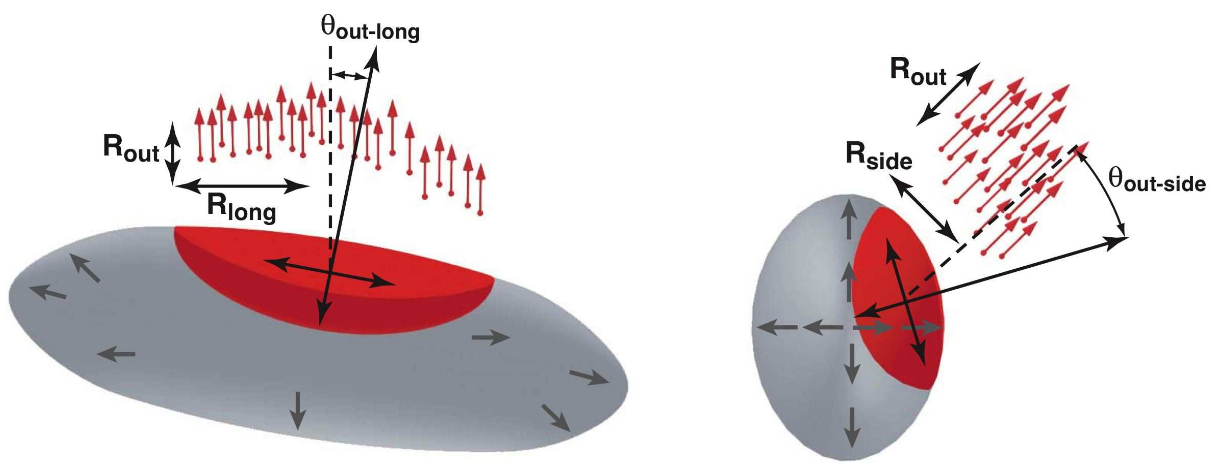
\includegraphics{hbt_radii_outsidelong.png}
  \caption{The HBT radii in the Bertsch-Pratt coordinate system \cite{Lisa:2005dd}. The longitudinal radius \Rlong is evaluated in the frame boosted to the pair's longitudinal momentum. The outwards transverse radius \Rout is along the pair's transverse momentum, and \Rside is the other transverse component.}
  \label{fig:hbt_outsidelong}
\end{figure}

The full HBT matrix is written out in this coordinate system as
\begin{equation}
  \label{eq:r_matrix_full}
  R = \left( \begin{array}{ccc}
  \Rout & \Ros & \Rol \\
  \Ros & \Rside & \Rsl \\
  \Rol & \Rsl & \Rlong
  \end{array} \right) \; .
\end{equation}
The main HBT radii are the diagonal terms of this matrix, illustrated in \cref{fig:hbt_outsidelong}.
The outwards radius \Rout represents the radial depth of the region of homogeneity as seen by the pair.
In hydrodynamic models the value of \Rout depends on the transverse velocity and the lifetime of the source.
The sideways radius \Rside is the transverse size of the source in the direction perpendicular to \kt.
The radius \Rlong indicates the longitudinal size of the region of homogeneity in the \ac{LCMF}.
Cross-terms \Ros, \Rol, and \Rsl are small relative to the main radii and in certain inclusive cases symmetries fix some or all of them to zero.

For identical particles the correlation function is symmetric under exchange of the pair, \(C(-\mathbf{q}) = C(\mathbf{q})\), so a single component of $\mathbf{q}$ can always be chosen as positive.
The order of a particle pair is picked such that $\qout > 0$.
Aside from the azimuthally-dependent results, the average azimuthal symmetry of the \pPb system is invoked so that $C(-\qside) = C(\qside)$, and it will be sufficient to consider only the absolute value $|\qside|$ and $\Ros = 0$.
In the azimuthally-dependent results, the \Rol term is sub-dominant compared to the other components\footnote{as shown in the results} and is fixed to zero, and only the absolute value of \qlong is considered.
In both cases $\Rsl = 0$.
In summary, for rapidity-dependent results only the \Rol cross-term is used
\[
R = \left( \begin{array}{ccc}
  \Rout & 0 & \Rol \\
  0 & \Rside & 0 \\
  \Rol & 0 & \Rlong
\end{array} \right) \;,
\]
and for the azimuthally-dependent results only \Ros is non-zero, with
\[
R = \left( \begin{array}{ccc}
  \Rout & \Ros & 0 \\
  \Ros & \Rside & 0 \\
  0 & 0 & \Rlong
\end{array} \right) \; .
\]

Motivated by the Gaussian parameterization\footnote{i.e. the L\'evy parameter $\alpha = 2$}, many results report the square of the matrix $R^2$ rather than the $R$ matrix defined here with units of length.
This must be accounted for when comparing results using different conventions.
Fortunately a comparison is simple when the cross-terms are relatively small, as
\begin{equation}
  R^2 = \left( \begin{array}{ccc}
  \Rout^2 & \Ros(\Rout+\Rside) & \Rol(\Rout+\Rlong) \\
  \Ros(\Rout+\Rside) & \Rside^2 & 0 \\
  \Rol(\Rout+\Rlong) & 0 & \Rlong^2
  \end{array} \right) + \bigo{ \Ros^2, \Rol^2, \Ros \Rol }
\end{equation}
with $\Rsl = 0$.

\subsection{HBT radii under collective flow}

The femtoscopic radii are not equivalent to the total size of the source but rather indicate the size of the region of homogeneity.
This volume is the effective size of the source with which particles have equilibrium.
Collective expansion makes it more difficult for two regions of the source to equilibrate as they are pushed apart from each other.
In an infinite volume the size of the region of homogeneity is set by the length scale at which collective velocity overcomes thermal velocity \cite{Lisa:2005dd} so
\begin{equation}
R_i \sim \frac{v_\textrm{thermal}}{\frac{du}{dx_i}}
\end{equation}
where the collective velocity is described by the function $u(x)$.

\begin{figure}[t]
  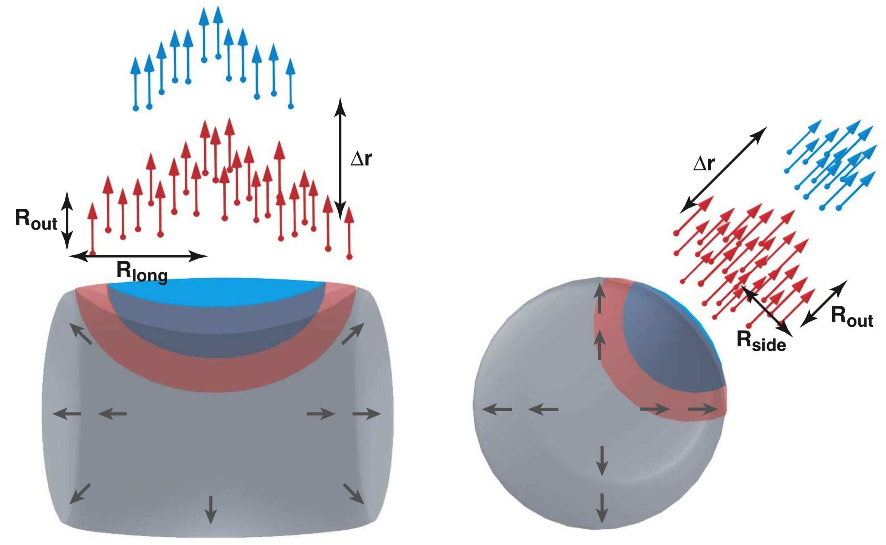
\includegraphics{hbt_radii_flow.png}
  \caption{Particles with a higher \pt give smaller values of \Rlong under longitudinal flow (left) and smaller values of the transverse radii under radial flow (right) \cite{Lisa:2005dd}.}
  \label{fig:hbt_flow}
\end{figure}

After a heavy ion collision the generated matter is spread longitudinally between the nuclear remnants with boundaries traveling away from the \ac{IP} at speed $c$.
The collective velocity profile is approximated as $u = z/t$ in the absence of longitudinal acceleration.
The longitudinal radius is then determined by the expected emission time
\begin{equation}
  \Rlong \approx v_\textrm{thermal} \langle t \rangle \; .
\end{equation}
The thermal velocity scales with $\sqrt{T/\mt}$ at large \mt where $\mt = \sqrt{m^2 + \pt^2}$ is the transverse mass.
However, because particles with larger \mt are typically emitted earlier \Rlong may be expected to decrease more rapidly than $1/\sqrt{\mt}$.

Transverse expansion is generated by the particular dynamics of the system, so the dependence of the transverse radii on \mt depends on the choice of blast wave model.
Generally a similar decrease with \mt is predicted for \Rout and \Rside as well as \Rlong, as shown in \cref{fig:hbt_flow}. Generally the decrease of femtoscopic radii with rising pair \kt is interpreted as a signature of collective expansion \cite{Kolb:2003dz}.

%% \cite{Kolehmainen:1986fe,Padula:1989ie} %% bjorken flow correlation function


\subsection{Motivation for femtoscopy in proton-lead collisions}
Femtoscopic measurements have already been made in \pPb collisions \cite{Abelev:2014pja,Adam:2015pya} but there is space for advancement.
The \kt-dependence of these measured HBT radii suggests collective expansion even in peripheral collisions.
However, this pattern is faked by the increasing relevance of jet fragmentation correlations at larger \kt and in peripheral collisions, and the method used to account for this background is susceptible to this bias.
Thus increasing sophistication in the methods used to constrain this background are desirable.
In addition, rapidity-dependent measurements of the radii have the potential to have nontrivial behavior in an asymmetric \pA system, and ATLAS is particularly well-suited to such a measurement with an inner detector covering 5 units of pseudorapidity.

Because femtoscopy provides a measurement of the source's spatial dimensions, it is particularly useful for probing the hydrodynamic prediction that spatial anisotropies lead to complementary momentum anisotropies.
Elliptic modulation of the freeze-out shape has been observed in \AuAu \cite{Adams:2003ra,Adare:2014vax,Adamczyk:2014mxp} and \PbPb \cite{Adamova:2017opl} collisions, which show that the transverse radii are reduced along the event plane axis compared to out-of-plane.
The second-order Fourier coefficient of \Rside is shown in \cref{fig:rside_v2_aa} for \AuAu and \PbPb systems as a function of the initial ellipticity computed in the MC Glauber model.
The final source ellipticity indicated by $\Rside{}_{,c2} / \Rside{}_{,0}$ has the same sign as the initial ellipticity but with a reduced magnitude.
This is consistent with an elliptic transverse source profile that expands more along the minor axis but not enough to overtake the length of the major axis.

\begin{figure}[t]
  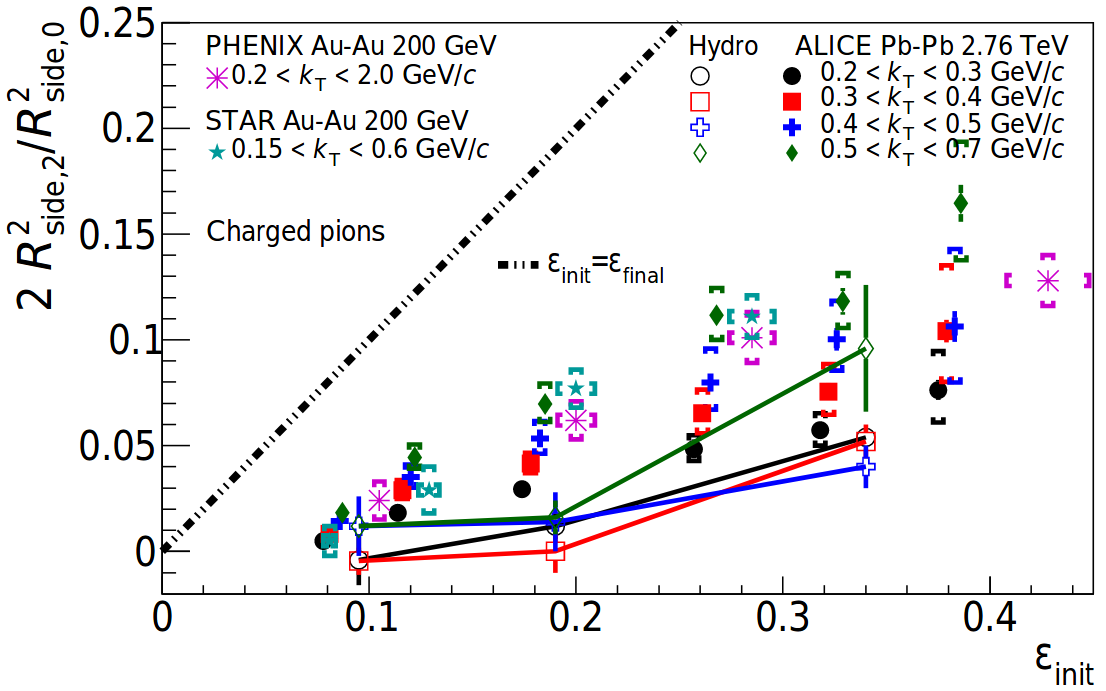
\includegraphics{azi_hbt_aa_ellipticity.png}
  \caption{The relative second-order Fourier coefficient of \Rside in nucleus-nucleus collisions compared to the initial source eccentricity calculated from the MC Glauber model \cite{Adamova:2017opl}.}
  \label{fig:rside_v2_aa}
\end{figure}

Azimuthal measurements are challenging outside of \AA collisions because the resolution of the event plane \psit depends heavily on the event activity.
ATLAS has a reasonably high event plane resolution in central \pPb events with reasonably large elliptic flow.
An observation of the same type of azimuthal dependence of the HBT radii that is observed in \AA collisions would provide compelling evidence for the hydrodynamic behavior of central \pPb collisions.
         % Theory and status of experimental results
\chapter{Experimental design and apparatus}
\label{ch:experiment}
\graphicspath{{Chapter-Experiment/figures/}}

\section{Scattering experiments}

\subsection{History and motivation}
The first modern scattering experiments were the Geiger-Marsden experiments in the early 1910s, in which the Rutherford scattering of alpha ($\alpha$) particles by gold foil was observed \cite{Rutherford:1911zz}.
While most $\alpha$ particles passed through the foil with little deflection, a small fraction of them were deflected to extreme angles (\cref{fig:rutherford}).
This result provided evidence that electric charge within the foil was not distributed uniformly, but localized in very small clusters -- the nuclei of the gold atoms.
\begin{figure}[t]
  %% https://www.chegg.com/homework-help/questions-and-answers/rutherford-s-experiment-studied-deflection-scattering-ofalpha-particles-known-helium-nucle-q458296
  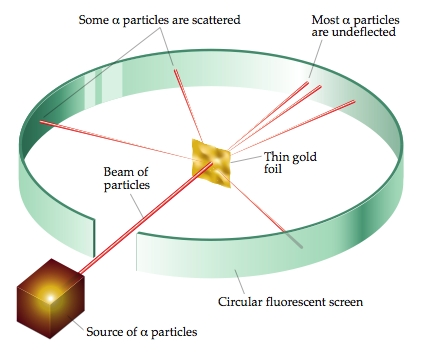
\includegraphics{BLB-1070873-Rutherford_v2.jpg}
  \caption{Rutherford scattering of alpha particles by gold foil, demonstrating the existence of the atomic nucleus.}
  \label{fig:rutherford}
\end{figure}

With elementary quantum mechanics, this type of elastic scattering can be understood more precisely.
In the Born approximation, which is essentially the weak-potential limit, the quantum amplitude $f$ of a particle with incoming momentum $\mathbf{p}_{i}$ scattering elastically off a target potential $V(\mathbf{x})$ with outgoing momentum $\mathbf{p}_{f}$ is proportional to the Fourier transform of the potential:

\begin{equation}
  f\left(\mathbf{p}_f ; \mathbf{p}_i\right) \propto - \int d^3 x \, V(\mathbf{x}) e^{-i \Delta \mathbf{p} \cdot \mathbf{x}}
  \label{eq:born}
\end{equation}
where $\Delta \mathbf{p} \equiv \mathbf{p}_f - \mathbf{p}_i$ is the momentum transferred to the projectile particle.
The differential scattering cross section $d\sigma/d\Omega$ (the scattering probability density per unit area) is given by the square of the quantum amplitude, so it is proportional to the squared magnitude of the Fourier transform of the potential.

\begin{equation}
  \frac{d\sigma}{d\Omega} \propto \left| \int d^3 x \, V(\mathbf{x}) e^{-i \Delta \mathbf{p} \cdot \mathbf{x} / \hbar} \right|^2 = \left| \tilde{V}(\mathbf{\Delta \mathbf{p}}) \right|^2
\end{equation}
Because the net momentum transfer is constrained by the relative momentum between projectile and target, larger momentum -- or equivalently, higher energy -- is required to probe the finer structure of the target.
This correspondence between center-of-mass energy and the spatial resolution of the probe remains valid even for inelastic collisions and strong interactions.
The required energy to probe a distance scale can be estimated with dimensional analysis.
To resolve the structure of a target down to a distance scale $l$, the center-of-mass energy $E$ is

\begin{equation}
E = \frac{\hbar c}{l} \approx \frac{0.2 \GeV \fm}{l} \; .
\end{equation}
Resolving individual atoms requires collisions with energy of order \keV, resolving the nucleus requires at least \MeV\ scale energies, and resolving sub-nucleic structure requires collisions of at least order \GeV.

\subsection{Accelerator physics}

%% \todo{define mandelstam variable $s$, motivate w/ Lorentz invariance. not necessarily here but somewhere} %% s is now defined in intro, but could be moved here
In a fixed-target experiment using target particles of mass $m_t$ and a projectile beam with particles of rest mass $m_p$ and energy $E$, the center-of-momentum energy $\sqrt{s}$ is given by
\begin{equation}
\sqrt{s} = \sqrt{(m_t+m_p)^2 + 2 m_t (E - m_p)} \; ,
\end{equation}
which scales with the square root of the beam energy even for large energies.
On the other hand, if two beams are accelerated and directed into each other, the center-of-momentum energy of each collision is
\begin{equation}
\sqrt{s} = \sqrt{(E_t + E_p)^2 - (|\mathbf{p}_t| - |\mathbf{p}_p|)^2} \; ,
\end{equation}
which scales linearly with the total energy, and is equal to $2E$ in the case where the beams are identical.
While fixed-target experiments were the first to be developed, they are not as efficient at reaching high energies as dual-beam colliders.
Modern high-energy experiments therefore accelerate two particle beams and generate collisions by intersecting the beams head-on.

\subsubsection{Accelerator designs}

\begin{figure}[t]
  %%  https://www.cyberphysics.co.uk/topics/atomic/Accelerators/LINAC/Linac.htm
  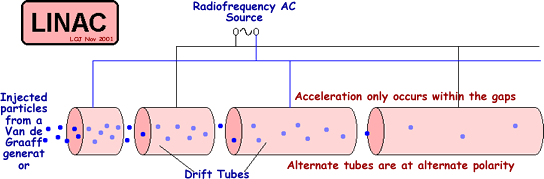
\includegraphics{LINAC.png}
  \caption{A linear accelerator.}
  \label{fig:linac}
\end{figure}

The most straightforward method to accelerate charged particles to high energies is to allow them to pass through a large voltage differential.
A large voltage can be produced, for instance, with a Van de Graaff generator \cite{PhysRev.43.149}.
The voltage differential is limited by the insulation breakdown, which in practice caps the energy of accelerated particles with charge $Ze$ to a few $Z \cdot\MeV$.
A modern \linac circumvents this issue by passing ions through a series of drift tubes with alternating positive and negative potentials (\cref{fig:linac}).
The drift tubes are constructed with conducting material, so they shield the ions traveling through them from external electric acceleration.
Between the drift tubes, however, strong electric fields are induced by the alternating potentials.
This voltage difference is oscillated with \rf and the apparatus is constructed such that ions injected at a given velocity can pass through each gap with acceleration in the forward direction.
The \ac{SLAC} hosts the largest linear accelerator, which began operation in 1966.
The 3 km long machine was capable of accelerating electrons and positrons to energies of up to 50 \GeV.
While this is several orders of magnitude higher than the energies accessible with a simple voltage differential, increasing the energy further requires proportional increases in the length of the accelerator, exacerbating technical difficulties in its placement, construction, and maintenance.

\begin{figure}[t]
 %% https://www.mpoweruk.com/figs/cyclotron.htm
  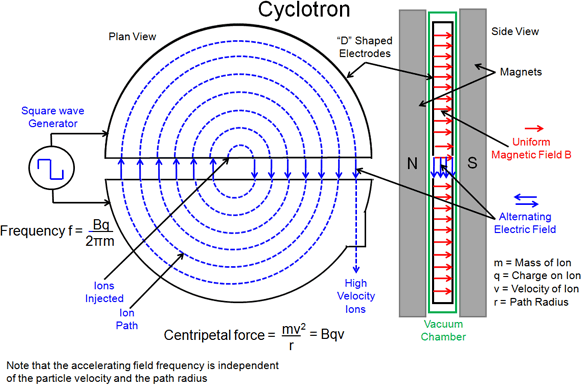
\includegraphics{cyclotron.png}
  \caption{A cyclotron.}
  \label{fig:cyclotron}
\end{figure}
The cyclotron is the next fundamental progression in accelerator technology.
Ions in a cyclotron are passed between two semi-cylindrical electrodes (``dees'') that are driven with an alternating voltage (\cref{fig:cyclotron}).
A large electromagnet keeps the particles traveling in a circular path contained within the dees.
At non-relativistic energies, the velocity of the ions is proportional to the radius of their path, so the time taken for one revolution is independent of the velocity.
If the voltage between the electrodes is oscillated with a frequency equal to the cyclotron resonance frequency $f_\textrm{cyclo} = q B / 2\pi m$, then ions are accelerated to higher energies with each pass between the dees.
At a fixed radius (and therefore fixed energy), the ion beam is allowed to exit the cyclotron.
Classically, the kinetic energy is proportional to the square of the radius, inviting a comparison to a hypothetically coiled \linac.
Relativistic energies can be attained with more sophisticated designs that vary either the frequency over time or the magnetic field with the radial position, but as the velocity approaches $c$ the energy is only linearly proportional to the radius:
\begin{align}
\label{eq:gyroradius}
E =& \; \frac{q B R c^2}{v}\\
\overrightarrow{{}_{v \rightarrow c}}& \; q B R c
\end{align}
This shows that the energies accessible from a circular accelerator are directly limited by the maximum strength of the magnetic field and the radius of the path.

The radius of a cyclotron design can only be increased so much before it becomes infeasible.
The synchrotron is a toroidal accelerator in which ion beams travel around the torus, turned by dipole magnets along the path.
Quadrupole and higher-multipole magnets are used to maintain the focus of the beam and make fine-tuning adjustments to the magnetic fields.
This layout does not permit particles to be accelerated from an arbitrarily small energy, so a synchrotron is generally filled with particles first accelerated from a \linac, and the ions are kept circling the path at the injection energy.
Once the beam pipe is filled, the energy of the ion beam is gradually increased by \rf cavities that oscillate to apply an acceleration to the particles.
The oscillation of the \rf cavities groups the ions into bunches along the beam.
The limiting factor for synchrotron performance depends on the mass of the particle; for electrons the power lost via synchrotron radiation $P_\textrm{synch-rad} \propto e^2 E^4 / m^4 R^2 $ is the limiting factor in the maximum energy.

\subsubsection{Luminosity}

The capability of an accelerator to provide collision events to a detector is characterized by its luminosity.
The rate of events $dN/dt$ of a given set of processes is proportional to the relevant cross-section of the collision participants $\sigma$.
The proportionality factor is defined as the instantaneous \emph{luminosity} \Lumi.
\begin{equation}
\label{eq:rate_lumi}
\frac{dN}{dt} = \sigma \Lumi
\end{equation}
This definition is useful because it separates the contributions to the rate of observations into the independent contributions from physics ($\sigma$) and from the accelerator (\Lumi).
The total number of events is proportional to the \emph{integrated luminosity} $\Lint = \int \Lumi \, dt$.
\begin{equation}
N = \sigma \Lint
\end{equation}
The quantity of data recorded in a time period is typically reported in terms of \Lint.

For two bunched beams colliding head-on with identical Gaussian transverse profiles the luminosity is
\begin{equation}
\Lumi = f_\mathrm{coll} \frac{n_1 n_2}{4 \pi \sigma_x^* \sigma_y^*}
\end{equation}
where the bunch crossings occur with frequency $f_\mathrm{col}$, there are $n_1$ and $n_2$ particles in each bunch, and $\sigma_x^*$ and $\sigma_y^*$ characterize the transverse beam size in the horizontal and vertical directions at the \ac{IP}.
The quadrupole focusing magnets are placed to alternatively squeeze the beam in the $x$ and $y$ directions.
This leads to oscillatory motion in the path $s$ following the Hill equation \cite{Tanabashi:2018oca}:
\begin{align}
x(s) =& \; A \sqrt{\beta(s)} \cos (\psi) \\
x'(s) =& \; \frac{A}{\sqrt{\beta(s)}} \left( \frac{1}{2} \frac{d\beta(s)}{ds} \cos(\psi) - \sin(\psi) \right)
\end{align}
where the phase $\psi$ is a function of $s$ and $d\psi(s)/ds = 1/\beta(s)$.
As long as the energy of the beam is constant, this trajectory traces a closed path in the phase space for each transverse direction, and the area of phase space is constant.
The emittance $\epsilon$ is defined as this phase space area,
\begin{equation}
\epsilon_x = \frac{\pi \sigma_x^2}{\beta_x} \; ,
\end{equation}
and similarly for the $y$ direction.
Then the luminosity can be expressed as a function of the emittance and $\beta^*$, the value of $\beta$ at the beam crossing.
\begin{equation}
\label{eq:lumi}
\Lumi = f_\mathrm{coll} \frac{n_1 n_2}{4 \sqrt{\epsilon_x \epsilon_y \beta_x^* \beta_y^*}}
\end{equation}
If the crossing angle is non-zero or $\beta$ is not minimized at the \ac{IP}, the real luminosity will be smaller than this optimal value. %% there are other effects that can decrease lumi but we aren't going into detail
\cref{eq:lumi} shows that the keys to increasing the efficiency of data-taking are to make highly-populated bunches cross at high frequency, with low-emittance beams and optics that minimize the amplitude functions at the \ac{IP}.

\section{The Large Hadron Collider}

The \lhc is a high-energy particle ring collider located near Geneva on the Swiss-French border \cite{LHCMachine}.
It was constructed by the European Organization for Nuclear Research (CERN, for ``Conseil européen pour la recherche nucléaire'') and is currently the highest energy particle accelerator in the world, with a design center-of-mass energy for proton collisions of \ppenergy.
Two adjacent beam pipes lie in a 26.7 km circumference and are filled in an anti-aligned orientation so that the beams can be crossed to generate collisions.
While it was primarily designed to provide proton-proton (\pp) collisions, it is also capable of colliding lead (${}^{208}_{\ 82}\textrm{Pb}$) and xenon (${}^{129}_{\ 54}\textrm{Xe}$) ions with themselves and with protons.
The results of this thesis will use data collected from the 2013 \pPb collisions, which were taken at a center-of-mass energy per nucleon of \pPbenergy.

\subsection{Injection chain}

\begin{figure}[t]
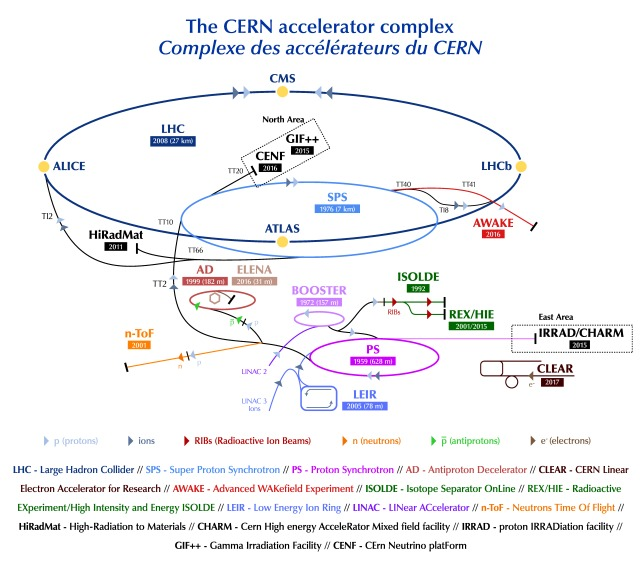
\includegraphics{CCC-v2018-print-v2.jpg}
\caption{The LHC is the last ring (dark blue line) in a complex chain of particle accelerators. The smaller machines are used in a chain to help boost the particles to their final energies and provide beams to a whole set of smaller experiments. (Copyright CERN \cite{Mobs:2636343})}
\label{fig:injection_chain}
\end{figure}

Before being injected into the \lhc, ion beams pass through a series of increasingly large accelerators, incrementally raising their energy \cite{Benedikt:2004wm}.
These lower-energy accelerators predate the \lhc and have each been used for many collision experiments throughout the history of CERN.
The CERN accelerator complex is sketched in \cref{fig:injection_chain}.

Protons are first collected by ionizing hydrogen gas, then accelerated to a kinetic energy of 50 \MeV\ by the Linac 2 linear accelerator.
The \ac{PSB} increases their energy to the relativistic level of 1.4 \GeV.
From there, the beam is energized in the \ac{PS} to 25 \GeV, then the \ac{SPS} to 450 \GeV.
These proton beams from the \ac{SPS} are used to fill the \lhc, where they are again accelerated to collision energies of a few \TeV each.

Lead ions are accelerated from rest by the Linac 3 linear accelerator, a dedicated ion \linac, to a kinetic energy of 4.2 \MeV per nucleon (\MeVn).
The \ac{LEIR} raises their energy to 72 \MeVn\ and also applies electron cooling to the ion beam.
This process involves merging the ions with an electron beam and allowing the mixture to come to thermal equilibrium so that the electron cloud absorbs thermal energy from the ions.
The ions are then re-separated from the electrons as they pass through a dipole magnet.
This cooling step, which effectively reduces the phase space volume of each bunch, is necessary to counteract the higher charge of the ions pushing them apart. %% equivalently, reducing the ``emittance'' of the beam
From the \ac{LEIR} the lead ion beam is injected into the PS, which raises its energy to 5.9 \GeVn, then the \ac{SPS}, which raises it to 177 \GeVn.
Finally, the beam is injected into the \lhc, where it is accelerated to a few \TeVn depending on the intended collision system.


\subsection{LHC main ring}

\begin{figure}[t]
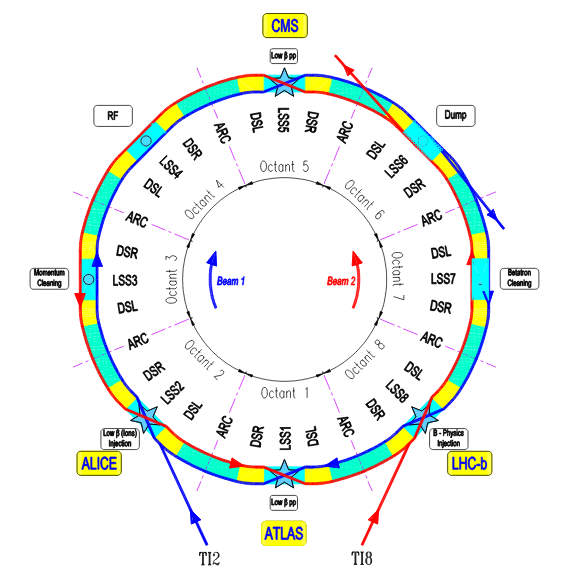
\includegraphics{LHC_schematic.png}
\caption{Schematic layout of the two beams of the \acs{LHC} \cite{Bruning:2004ej}.}
\label{fig:lhc_schematic}
\end{figure}

The \lhc ring does not trace a perfect circle, but is actually composed of eight alternating straight and curved arc sections through which pass two parallel beam pipes (\cref{fig:lhc_schematic}) \cite{Bruning:2004ej}.
The straight sections are each 528 m in length and contain the \rf cavities for acceleration, \acp{IP} for colliding beams at the various detector sites, and other features like injection spots and beam dumps.
The arc portions have a radius of curvature of $R = 2.8$ km and use a total of 1232 superconducting dipole magnets to turn the beams along the path.

The \rf cavities operate at 400 MHz, which corresponds to \rf buckets of 2.5 ns.
For ultra-relativistic beams, this corresponds to a minimum length spacing between bunches of 0.75 m.
Practically, however, the injection from the \ac{SPS} limits the bunch spacing to multiples of 25 ns, or 7.5 m separation.
The \lhc can thus fit a maximum of 3560 bunches in each of its rings, but they are not completely filled because gaps need to be left to allow safe beam dumps.
As of 2018, the smallest bunch spacing used for lead ions is 75 ns.

\begin{figure}[t]
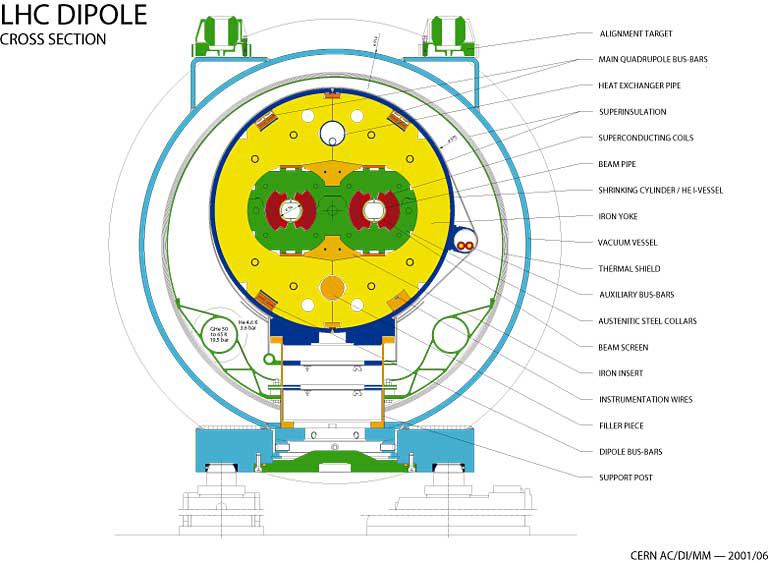
\includegraphics{LHC-PHO-2001-187.jpg}
\caption{A dipole magnet used to turn the beams along an arc. The two beams travel in the evacuated beam pipes running anti-parallel to each other, which requires the magnetic field in each to be opposite. (Copyright CERN \cite{Valeriane:843195})}
\label{fig:dipole_cross_section}
\end{figure}

The dipole magnets (\cref{fig:dipole_cross_section}) have a maximum design strength of 10 T, although the active field strength must remain proportional to the current energy of the beam fill.
For the \pPbenergy \pPb run they operated at 6.0 T with fully energetic beams.
\todo{beams @ fixed rigidity, explain different energies in beams, different Z/A. possibly move some details from 3.2.4 up here}
To keep the beams focused, 392 quadrupole magnets are arranged in an alternating-polarity orientation.
This scheme alternately squeezes the beams horizontally and vertically, with a net effect of keeping the beam radius small.
Over 6000 additional multipole magnets are used for fine-tuning the magnetic fields.
The electromagnets use niobium-titanium (NbTi) as the conducting material, which has a critical temperature of 10 K and a maximum critical magnetic field of 15 T.
They are cooled with superfluid liquid helium (${}^{4}\textrm{He}$) to a temperature of 1.8 K.
A failure in the cooling system that allows the magnet temperature to rise above its critical temperature causes it to quench.
The increase in resistance from the loss of superconductivity causes a rapid temperature increase.
This is particularly disastrous if the helium is heated to its gaseous phase, causing it to explode\footnote{This actually occurred at the \lhc in September of 2008, delaying operations for over a year.}.


\subsection{LHC experiments}
The two largest \lhc experiments, ATLAS\footnote{an ``acronym'' for \textbf{A} \textbf{T}oroidal \textbf{L}HC \textbf{A}pparatu\textbf{S}} \cite{Aad:2008zzm} and CMS\footnote{\textbf{C}ompact \textbf{M}uon \textbf{S}olenoid} \cite{Chatrchyan:2008aa}, are general-purpose detectors that fulfilled one of their primary objectives with the joint discovery of the Higgs boson in 2012 \cite{HIGG-2012-27,Chatrchyan:2012xdj}.
They continue to be used in the search for physics beyond the Standard Model such as supersymmetry and large extra dimensions.
The large rapidity coverage of their calorimeter and tracking systems also make them highly capable of measuring both low- and high-energy probes of heavy ion collisions.
The ATLAS detector, which provided the data used in this thesis, is discussed in more detail in \cref{sec:atlas}.

Other than ATLAS and CMS, the \lhc houses a number of other experiments that are more specialized for specific purposes.
ALICE\footnote{\textbf{A} \textbf{L}arge \textbf{I}on \textbf{C}ollider \textbf{E}xperiment} \cite{Aamodt:2008zz} is a dedicated heavy-ion detector that is particularly adept at the identification of particle species.
With many subdetectors spread over a forward region from its \ac{IP}, the LHCb\footnote{\textbf{LHC b}eauty} experiment \cite{Alves:2008zz} can make detailed measurements of the decay products of b-quarks. Recently it has led to the observation of possible pentaquark states \cite{Aaij:2015tga}.
TOTEM\footnote{\textbf{Tot}al Cross Section, \textbf{E}lastic Scattering and Diffraction Dissociation \textbf{M}easurement at the LHC} \cite{Anelli:2008zza} has detectors in the forward region over 200 m on either side of the CMS \ac{IP}.
Its location near the beam pipe puts it in a position to detect the products of elastic and diffractive collisions, which are characterized by a lack of color connection that would otherwise produce particles in the mid-rapidity region.
The LHCf\footnote{\textbf{LHC f}orward} experiment \cite{Adriani:2008zz} has two detectors along LHC beamline at 140 m away from the ATLAS \ac{IP} on either side.
The latest experiment to join the ring is MoEDAL\footnote{the \textbf{Mo}nopole and \textbf{E}xotics \textbf{D}etector \textbf{A}t the \textbf{L}HC} \cite{Acharya:2014nyr}.
It is a mostly passive detector located next to LHCb, with the goal of direct detector of magnetic monopoles or other stable massive particles beyond the Standard Model.

\subsection{Dataset provided}

\begin{figure}[t]
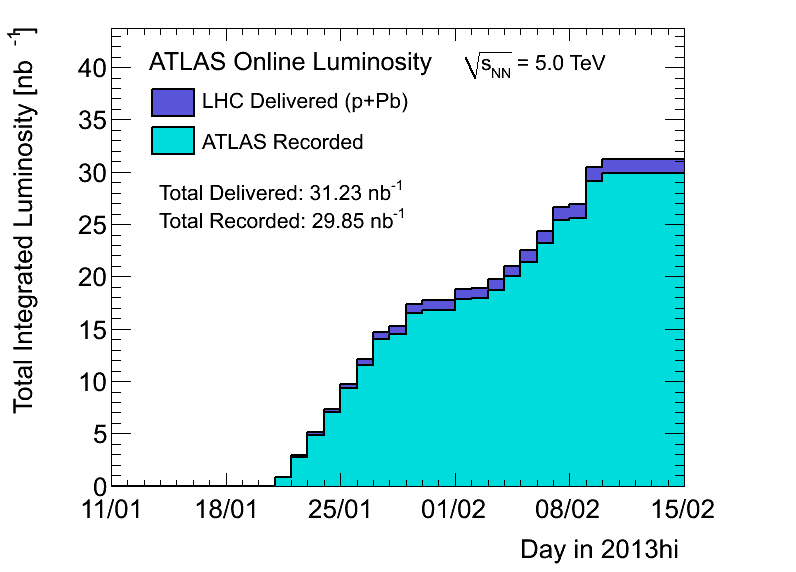
\includegraphics{sumLumiByDayUrgent.png}
\caption{The total integrated luminosity over the 2013 proton-lead data taking period.}
\label{fig:int_lumi}
\end{figure}

The results in this thesis use the 2013 \lhc \pPb dataset at a center-of-mass energy per nucleon of \pPbenergy.
The proton beam had an energy of 4 \TeV and the Pb ions had an energy per nucleon of $Z/A \cdot 4 \TeV = 1.57 \TeV$, so the center-of-mass of a proton and any one Pb nucleon had a longitudinal rapidity boost of $\ycm = 0.465$.
The \pPb run was divided into two periods between which the directions of the proton and lead beams were reversed to allow for better control over various systematic effects.
The maximum luminosity was $\Lumi_\textrm{peak} = 110 \times 10^{27} \, \textrm{cm}^{-2} \, \textrm{s}^{-1}$ over the 32 stable beam runs (16 in each period), though depending on the run $\Lumi_\textrm{peak}$ was as low as $22 \times 10^{27} \, \textrm{cm}^{-2} \, \textrm{s}^{-1}$.
The integrated luminosity of the data taking period from January 21 to February 10 is $\Lint = 28.1~\inb$ (\cref{fig:int_lumi}).
The bunch spacing of the beams was 200 ns, so the maximum bunch crossing rate was 5 MHz.

\section{The ATLAS detector}
\label{sec:atlas}

\begin{figure}[t]
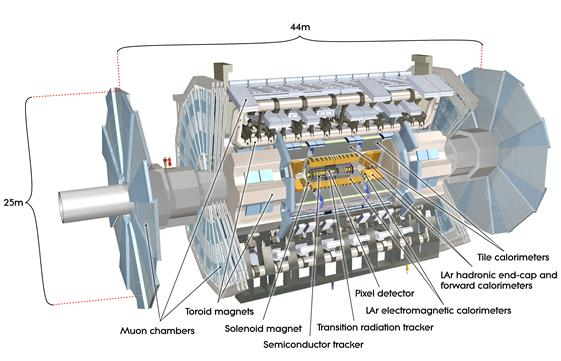
\includegraphics{ATLAS_layout.jpg}
\caption{The ATLAS detector and major subsystems. (Copyright CERN \cite{Pequenao:1095924})}
\label{fig:atlas_layout}
\end{figure}

The ATLAS experiment is a general purpose particle detector \cite{Aad:2008zzm} located at Point 1 on the \lhc ring, across the street from the main entrance to the CERN site at Meyrin, Switzerland.
Currently the largest volume accelerator detector in operation, it encompasses 44 m along the beam axis, has a diameter of 25 m, and weighs about 7 kilotonnes (\cref{fig:atlas_layout}).
Broadly speaking, the major subsystems of the ATLAS detector are (from inner- to outer-most): the \id, the magnet system, the calorimeters, and the muon spectrometer.
The muon spectrometer is essential for reconstructing a number of massive and exotic particles \cite{ATLAS:1997ad}; however, it will not be discussed in detail here as it is not used in the analyses presented in this thesis.
The extensive trigger and data acquisition system is also crucial for successful operation.
The \mbts detector sits on each side at a rapidity of $2.1 < |\eta| < 3.84$.
It is used to identify and trigger on minimum bias collisions.
The \zdc detectors are placed approximately 140 m on either side of the nominal \ac{IP} with a pseudorapidity of $|\eta| > 8.3$.
They are used to distinguish pileup events by detecting spectator nucleons that do not participate in the interaction.


\subsection{Magnets}
\label{subsec:atlas_magnet}

\begin{figure}[t]
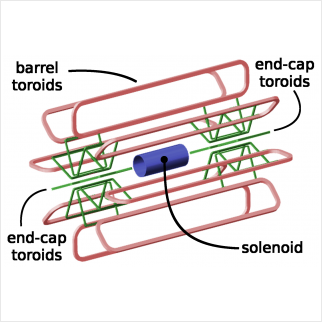
\includegraphics{atlas_magnets.png}
\caption{A schematic of the ATLAS magnet system. Copyright CERN}
\label{fig:atlas_magnets}
\end{figure}

Two superconducting magnet systems are used to generate a large magnetic field with field lines parallel to the beam axis (\cref{fig:atlas_magnets}) \cite{ATLAS:1997ae}. %% tech design report
This magnetic field causes charged particles to follow a curved path through the detector, allowing their charge and transverse momentum to be measured according to \(  \pt = q B_z R\) where $R$ is the radius of curvature in the transverse plane.
A large solenoid 5.3 m in length and 2.3 m in diameter surrounds the ID and produces a 2 T magnetic field.
It is designed to produce as uniform of a magnetic field as is possible to allow precise measurements of the momentum of charged particles in the ID.
The toroid magnet system consists of 8 air-core coils in the barrel and two sets of 8 air-core toroids in each of the end-caps.
The magnetic field produced by these is non-uniform but bends charged particles outside of the ID for measurements by the muon spectrometer.

\subsection{Inner detector}
\label{subsec:atlas_id}

\begin{figure}[t]
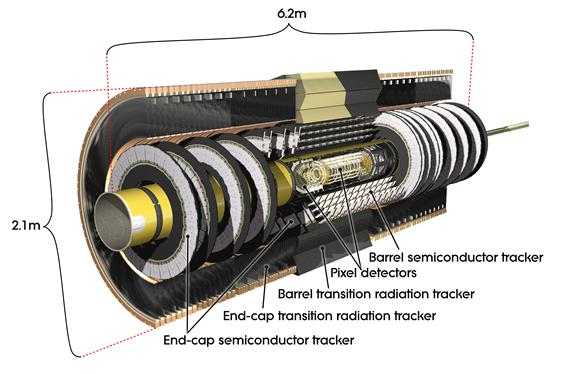
\includegraphics[width=0.57\linewidth]{id_whole.jpg}
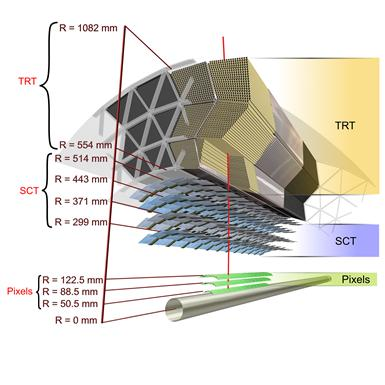
\includegraphics[width=0.42\linewidth]{id_slice.jpg}
\caption{Computer-generated images of the ATLAS inner detector. The left figure is a labeled graphic of the entire inner detector, and the right figure shows a cross-section of the barrel region. (Copyright CERN \cite{Pequenao:1095926})}
\label{fig:atlas_id}
\end{figure}

The ATLAS \id is designed to track the charged particles from collisions on their path from the beam pipe to the calorimeters, thereby inferring their charge and momentum \cite{ATLAS:1997ag,ATLAS:1997af,Aad:2010bx}.
It has a wide pseudorapidity coverage of \(\left| \eta \right| < 2.5\) and full azimuthal coverage in $\phi$.
The design resolution for the transverse momentum is \( \sigma_{\pt}/\pt = 0.05\% \, \pt /1 \GeV \oplus 1\% \), with a transverse impact parameter resolution of \( \sigma_{d_0} = 10 \mu\textrm{m}\) for tracks with a central rapidity.
Three sub-detectors are used, each in their own layer around the beam line.
From innermost to outermost, these are the silicon pixel detector, the \sct, and the \trt.


\subsubsection{Pixel detector}

The silicon pixel detector surrounds the beam pipe, covering radial distances from 50 mm to 150 mm, and is composed of 1744 silicon pixel modules \cite{Aad:2008zz}.
These are distributed over three concentric barrel layers and three disk layers on each endcap (\cref{fig:atlas_pixel}), so that the trajectory of a typical charged particle passes through three points in the pixel detector.
Each module is 16.4 mm by 60.8 mm and has 47 232 pixels of size 50 $\mu$m by 400 $\mu$m.
A total of 80.4 million readout channels are supported by 16 radiation-hardened front-end chips bump-bonded to each sensor.
A hit is recorded in each pixel when the signal exceeds a tunable threshold, and the time over threshold can be used to provide a measurement of ionization energy loss \dEdx used for particle identification.

\begin{figure}[t]
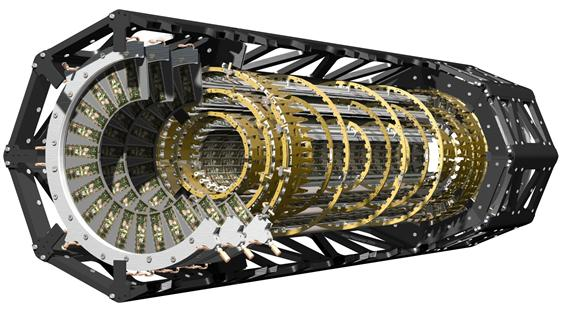
\includegraphics{pixel.jpg}
\caption{Computer-generated cutaway of the Pixel subdetector of the ATLAS inner detector. (Copyright CERN \cite{Pequenao:1095925})}
\label{fig:atlas_pixel}
\end{figure}


\subsubsection{Semi-conductor tracker}

The \sct consists of 4088 silicon-strip modules and covers a radial distance of 299 mm to 560 mm \cite{Aad:2014mta}.
These are placed in four concentric barrel layers and two endcaps of nine disks each.
A typical particle originating from the beam interaction region gets eight strip measurements in four space-points.
Most modules have four silicon-strip sensors, with two on each side glued back-to-back at a stereo angle of 40 mrad.
The relative angle between strips give space-points at the crossings.
The sensors are daisy-chained together to form 768 strips each with a length of 12 cm.
A total of 6.3 million readout channels are provided by radiation-hardened front-end readout chips.

\subsubsection{Transition radiation tracker}

The \trt covers the region from 563 mm to 1066 mm away from the beam line.
It consists of 298 304 proportional drift tubes (straws) each 4 mm in diameter \cite{Abat:2008zza}.
The straws are arranged in three cylindrical layers in the barrel region and are radially oriented in 80 wheel-like modules in the endcaps.
A typical track with $\pt > 0.5~\GeV$ and $|\eta| < 2.0$ crosses more than 30 straws.
There are a total of 350 848 readout channels.
The \trt hits are generally useful to refine the transverse momentum measurements of tracks seeded in the inner sub-detectors.

\subsection{Calorimetry}
\label{sec:atlas:calo}

\begin{figure}[t]
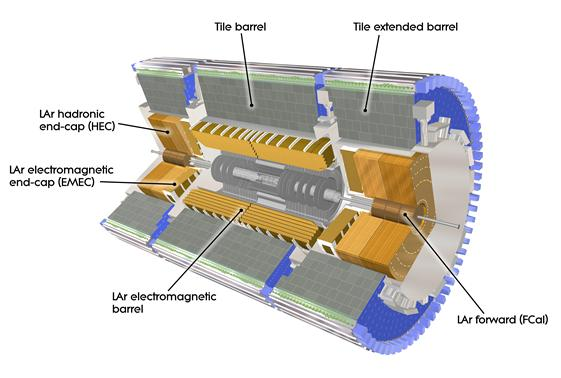
\includegraphics{calorimeter.jpg}
\caption{Computer-generated image of the ATLAS calorimeter systems. (Copyright CERN \cite{Pequenao:1095927})}
\label{fig:atlas_calorimeter}
\end{figure}

The ATLAS calorimetry system (\cref{fig:atlas_calorimeter}) covers nearly ten units of pseudorapidity at $|\eta| < 4.9$.
It provides measurements of high-energy particles by sampling the energy deposited in the calorimeters' dense active material \cite{Airapetian:1996iv}. %% performance tech design report
An absorbing material, placed in alternating layers with the active material, collects this energy from the showers.
ATLAS has two main categories of calorimeter, \emph{electromagnetic} and \emph{hadronic}.
The former is designed to induce \ac{EM} showers from electrons and photons, and the latter is designed to stop hadrons like protons and neutrons with both strong and \ac{EM} interactions.

\subsubsection{Electromagnetic calorimeter}

The electromagnetic calorimeter is the innermost calorimeter layer and covers the region $|\eta| < 3.2$.
It is divided into a barrel region at $|\eta| < 1.475$ and an end-cap at $1.375 < |\eta| < 3.2$, both of which use \ac{LAr} as an absorbing material \cite{ATLAS:1996ab} and lead as an active material. %% liquid argon
Electrons and positrons lose energy primarily through bremsstrahlung, radiating photons as they are slowed \cite{Fabjan:2003aq}.
Photons are stopped by the \ac{EM} calorimeter via pair production of electron-positron pairs.
A single electron or photon passing through the \ac{EM} calorimeter causes an electromagnetic cascade as these processes are repeated by product particles with progressively smaller energies.
As the energy is dispersed through the increasing number of shower particles, they are eventually slowed to a critical energy below which they interact through ionization and excitation, depositing their energy in the material.
The energy as a function of path length $\Delta l$ can be described by exponential decay \(E = E_0 e^{-\Delta l / X_0} \).
A typical photon or electron has a trajectory that, if extended beyond absorption, would cross a minimum of about 25 radiation lengths $X_0$ (\cref{fig:atlas_em_rad_length}).

\begin{figure}[t]
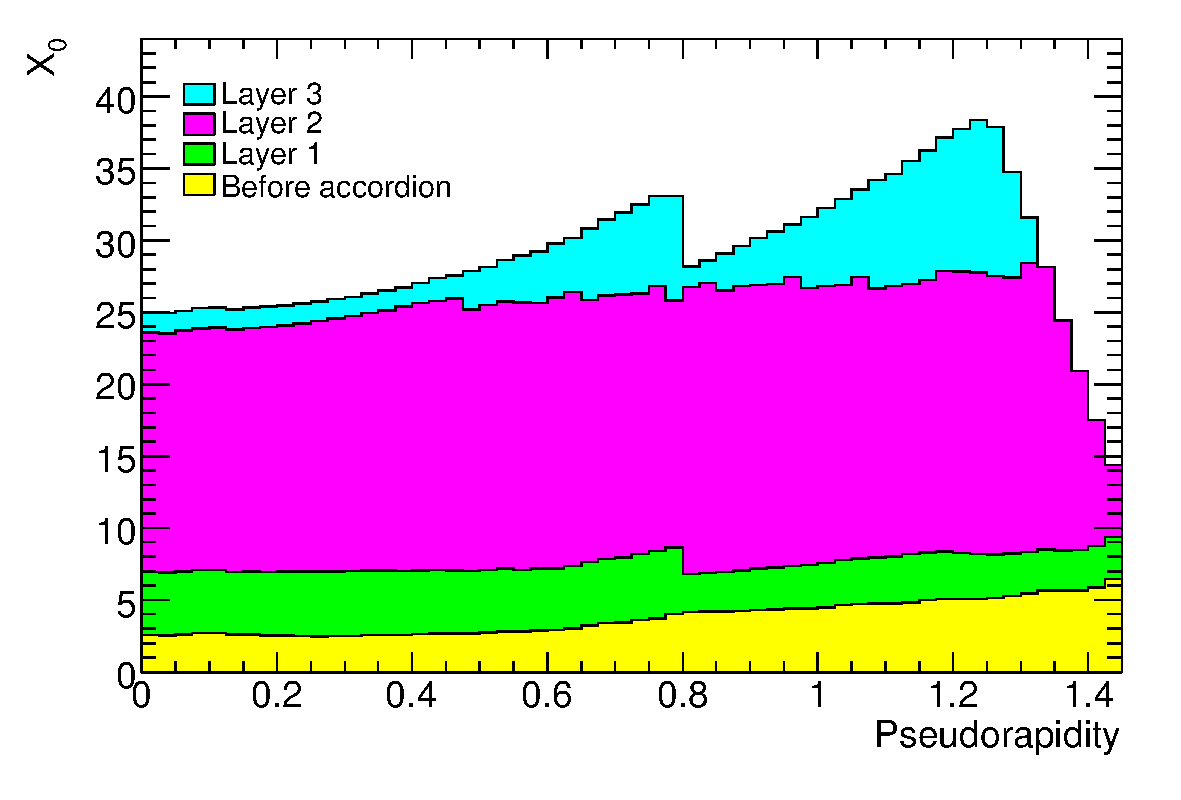
\includegraphics[width=0.49\linewidth]{x0_layers_barrel.pdf}
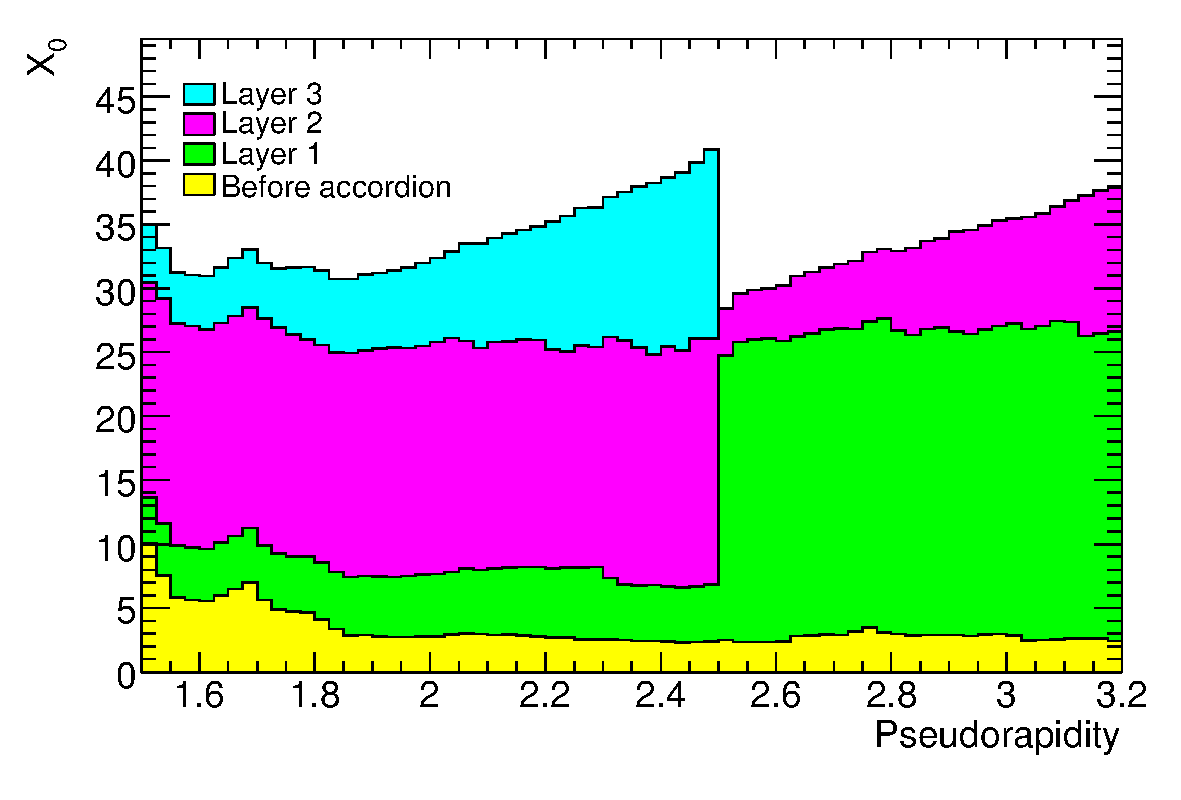
\includegraphics[width=0.49\linewidth]{x0_layers_endcap.pdf}
\caption{Thickness of the electromagnetic calorimeters in radiation lengths $X_0$ as a function of absolute pseudorapidity $|\eta|$ in the barrel (left) and end-cap (right) regions.}
\label{fig:atlas_em_rad_length}
\end{figure}

%% could talk about resolution following the Fabjan:2003aq ref

\subsubsection{Hadronic calorimeter}

The hadronic calorimeter lies outside the \ac{EM} calorimeter and is designed to stop protons and neutrons as well as the remnants of \ac{EM} cascades that are not completely absorbed by the \ac{EM} calorimeter.
The barrel region, along with the extended barrel region which encompasses the end-cap, cover $|\eta| < 1.7$ and comprise the tile system \cite{ATLAS:1996aa}.
The tile system does not use a \ac{LAr} active material, but rather is made of alternating steel plates and polystyrene scintillating tiles.
The \ac{HEC} detector covers $1.5 < |\eta| < 3.2$ and uses a \ac{LAr} active material with copper absorbers.
Most hadrons take a path that, if extended beyond the cascade, would cross at least 10 nuclear interaction lengths (\cref{fig:atlas_calo_nuclear_int_length}).

\begin{figure}[t]
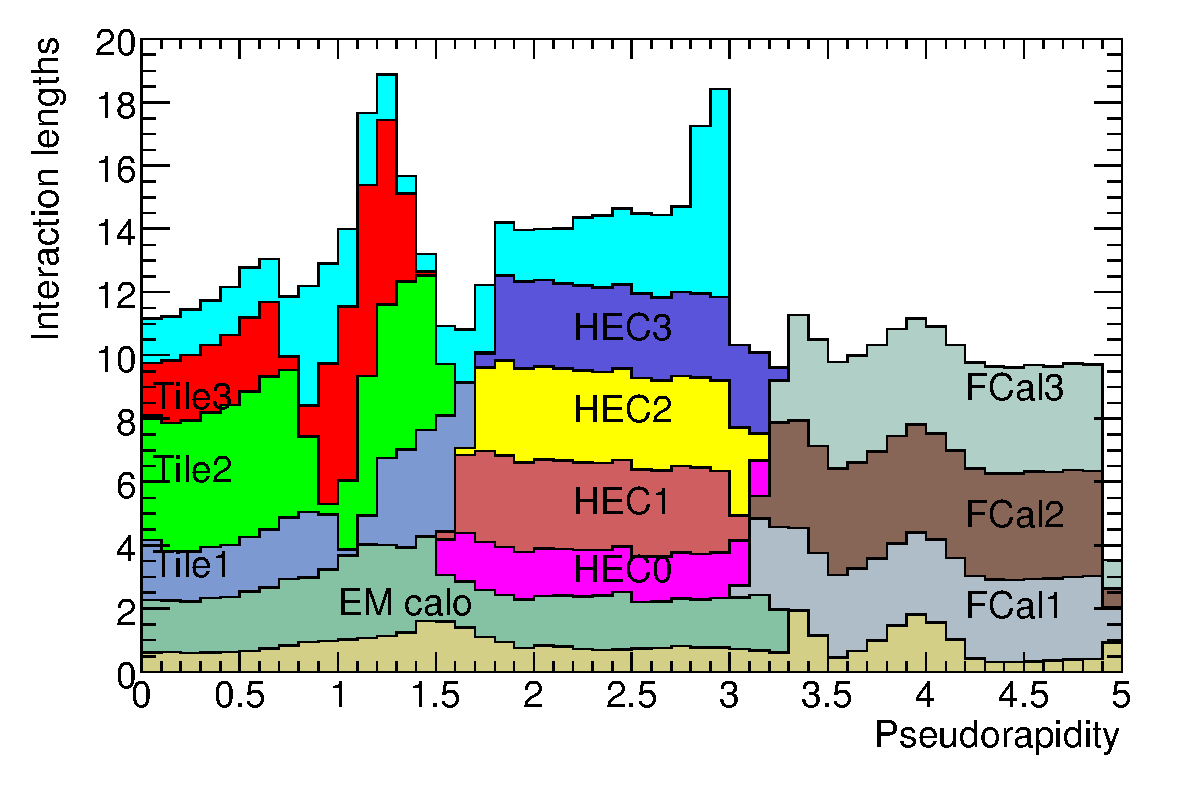
\includegraphics{calo_nuclear_int_length.pdf}
\caption{Nuclear interaction lengths for the combined ATLAS calorimetry system as a function of absolute pseudorapidity $|\eta|$.}
\label{fig:atlas_calo_nuclear_int_length}
\end{figure}

The hadronic cascade produced in the hadronic calorimeter is in some ways analogous to an \ac{EM} shower, though the interactions are mostly through the strong force.
Hadrons interact with the material and produce secondary particles that in turn produce their own shower, and energy is successively dispersed throughout the products.
The relative complexity of hadronic and nuclear processes makes a precise description more difficult since there are a greater number of relevant particles and nuclear resonances.
Sophisticated \mc simulations, using detailed models of the nuclear interactions, are required to accurately describe the physics of hadronic calorimeters.

\subsubsection{Forward calorimeter}
The \fcal consists of three layers situated underneath the endcap calorimeters at $3.1 < |\eta| < 4.9$.
It uses \ac{LAr} as its active material.
The first layer is designed for electromagnetic calorimetry and uses copper as its absorbing material, while the remaining two layers at larger $|z|$ are intended primarily for hadronic calorimetry and use tungsten as their absorbing material.
Due to its location in the forward region near the beam pipe the \fcal receives a greater amount of radiation than the other calorimeters.
In heavy ion collisions the \fcal is useful for measuring the centrality and reaction plane of events.

\subsection{Trigger}
%% \subsection{Trigger and data acquisition systems} %% maybe we don't need to get into DAQ
\label{subsec:atlas_trigger} % is it even worth labeling these if they're not numbered?

%% 200 ns for Pb; low mu reduces collisions
The \lhc can deliver a bunch crossing as often as the bunch spacing time, which was 200 ns for the \pPb run but can be as rapid as 25 ns for \pp collisions.
It is infeasible to record full events at the corresponding rate of up to 40 MHz, and many of the bunch crossings have cosmic backgrounds, out-of-time pileup\footnote{The \lhc \rf has a frequency of 2.5 ns, but the timing is designed to only fill a bunch every 25 ns. Stray particles can still find their way into unintended \rf buckets, causing out-of-time pileup when they collide at the \ac{IP}.}, or no collision at all.
Therefore the ATLAS trigger system needs to be capable of rapidly evaluating whether the data from an event is worth recording \cite{Aad:2012xs}. %% reference to performance paper
The trigger system has three levels, each of which processes the data and filters events for the next level.

The \ac{L1} trigger is a low-level hardware system that makes rapid determinations based on activity in the calorimeters, \mbts, \zdc, and muon spectrometers \cite{ATLAS:1998ad}.
It uses parallel data pathways separate from the regular readout path, with electronics optimized for speed over precision.
The \ac{CTP} combines the \ac{L1} trigger signals into combinations of \ac{L1} bits which are used to seed the \ac{L2} trigger.

The software-based \ac{HLT} is composed of the remaining two trigger levels, the \ac{L2} trigger and \ac{EF} \cite{ATLAS:2003aa}.  %% high-level trigger and DAQ
The \ac{L2} trigger uses regions of interest determined by the \ac{L1} trigger to seed algorithms that perform a more precise evaluation of the events.
The items from the \ac{L2} trigger processing are passed to the \ac{EF}, which uses the full offline readout path in order to mitigate biases from the ultra-fast \ac{L1} response.
An event is potentially recorded if it is selected by a trigger chain, which is defined by a \ac{L1} seed with \ac{HLT} items.
Recording every event that satisfies a trigger chain would still overwhelm the data acquisition system.
Prescales can be applied for items at any level in a trigger chain.
A trigger item with a prescale of $N$ is only flagged to be recorded at every $N$th instance of the trigger item firing.
The prescales of each trigger item are adjusted based on the physics goals of the run.

While many analyses of high energy data focus on the behavior of exceptional or rare events, the results presented in this thesis are concerned primarily with \minbias events.
The physics of interest is the bulk dynamics of the events on average rather than jets or rare particle decays.
General high-multiplicity and high-transverse-energy triggers are used to supplement the size of the data sample for central events.
These triggers are only used in the regime where their efficiency is practically 100\%, so the details of their performance are not as crucial here as they might be elsewhere.
         % Description of experimental apparatus
\chapter{Charged pion reconstruction and identification}
\label{ch:reconstruction}
\graphicspath{{Chapter-Reconstruction/figures/}}

Charged particles produced in collisions at the ATLAS \ac{IP} travel helical paths through the \id due to the solenoid magnetic field.
The three subdetectors register hits at various space-point locations as each of these particles passes through them, often 11 silicon and 15--30 \trt hits for a typical particle of sufficiently high \pt.
The trajectories of these particles must be reconstructed from the collection of all the space-point hits in order to infer the initial momentum of all of the collision products.
This procedure is non-trivial and computationally intensive, particularly because the trajectories of charged particles are altered when they pass through detector elements, via ionization energy loss and multiple scattering.

\section{Tracking algorithm}

%% for general track fitting overview see:
%% http://www.phys.ufl.edu/~avery/fitting.html
%% atlas overview see https://cds.cern.ch/record/1435196/files/ATLAS-CONF-2012-042.pdf
%% from \cite{ATLAS:2012jma}

%% discuss seeding before kalman filter?
%% i.e. split into ``pattern finding'' and ``track fitting'', though with NEWT there is ``no clear border'' between these modules
%% discuss inside-out and outside-in separately?

While the classification is not absolute, the ATLAS track reconstruction procedure can be divided roughly into two parts: first track seeds are identified, then tracks are extended and evaluated with a global fit \cite{Cornelissen:2007vba}. %% ATLAS new tracking (NEWT)
Each of these procedures will be described separately in the following sections.
Overall, the reconstruction of collision vertices and the charged-particle products has very good performance, even in the high-luminosity environment of the \lhc with tens of simultaneous collisions along the beamline \cite{ATLAS:2012jma}. %% performance of tracking and vertexing (2012), w/ description of reconstruction

\subsection{Seeding track candidates}

\begin{figure}[t]
  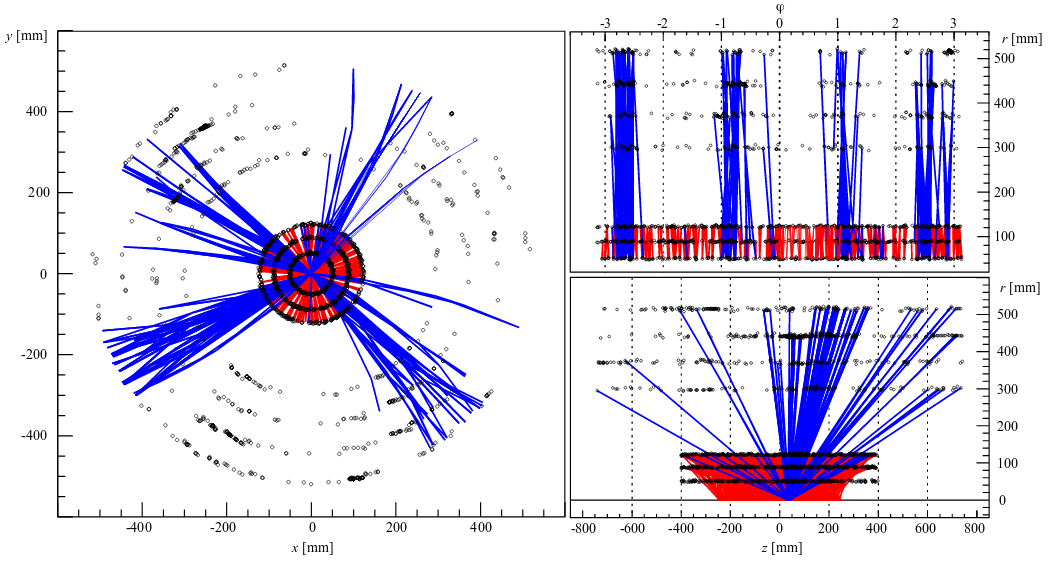
\includegraphics[width=\linewidth]{soft-pub-2007-007_sp_seeds.png}
  \caption{Space-point seeds constructed from two (short, in red) or three (long, in blue) hits in the barrel region of the pixel and \sct. Short seeds are used to determine the $z$-coordinates of predicted vertex positions, which are used to constrain extensions to three or more space points.  (From \Ref{\cite{Cornelissen:2007vba}})}
  \label{fig:trk_seeds}
\end{figure}

The baseline track finding algorithm uses inside-out reconstruction.
Space-points are collected by hits in the silicon detectors by the 3D location of pixel hits and by the crossing point of back-to-back \sct strip pairs with simultaneous hits.
Pairs of space-points from the pixel detector are used to construct short track seeds, which are used to find the longitudinal position of vertices.
A histogram is filled with the $z$-coordinate of straight-line extensions of these track seeds to the beam line and peaks in this distribution are identified with the $z$ position of the vertices.
These $z$-vertices constrain the extension of seeds from two space-points to three (\Cref{fig:trk_seeds}).
The seed search can also be done without the $z$ vertex constraint, inducing a significant increase in computational demands but allows for a greater efficiency to reconstruct decays from certain events.
The seeds with three space-points are fed to the track extension and fitting algorithm.

After the inside-out track reconstruction is completed, an additional round of seeding is performed using an outside-in algorithm called back-tracking.
This process is designed to reconstruct secondary particles, which are generated in the decays of primary particles and so do not necessarily originate from near the beam line.
The \trt drift tube hits do not provide fine-scale information along the straw direction, so seeds are built in the $r - \phi$ plane in the \trt barrel and the $r - z$ plane in the \trt end-cap.
Back-tracking is not well-suited for low-\pt particles, which spiral out of the \id without making it to the \trt, so the targeted particles have reasonably straight-line trajectories.
The Hough transform \cite{Duda:1972:UHT:361237.361242} is used to detect straight-line sets of three \trt hits which are used as track candidate seeds.
The extension of these \trt segments into the silicon detectors are evaluated in multiple $\eta$ slices to accommodate the fact that the seed-finding is done in the transverse plane.

Finally, the remaining silicon hits that have not been used in the inside-out or back-tracking algorithms are used to seed an additional low-\pt track reconstruction.%% ATL-COM-INDET-2012-052 for minbias
Charged particles with $\pt < 400 \MeV$ do not necessarily pass through every layer of the \sct.
These tracks can have a transverse momentum as low as 100 \MeV~ so their transverse radius of curvature is small.
Without a trajectory that is close to a straight line in the transverse plane, a larger set of possible track seeds must be evaluated, so it is only computationally feasible to seed the low-\pt tracking with leftover space-points from the other two tracking algorithms.
The efficiency below $\pt = 400 \MeV$ begins do fall rapidly with decreasing \pt, but a significant fraction of particles in this kinematic region are reconstructed.

\subsection{Track extension and fitting}

\begin{figure}[t]
  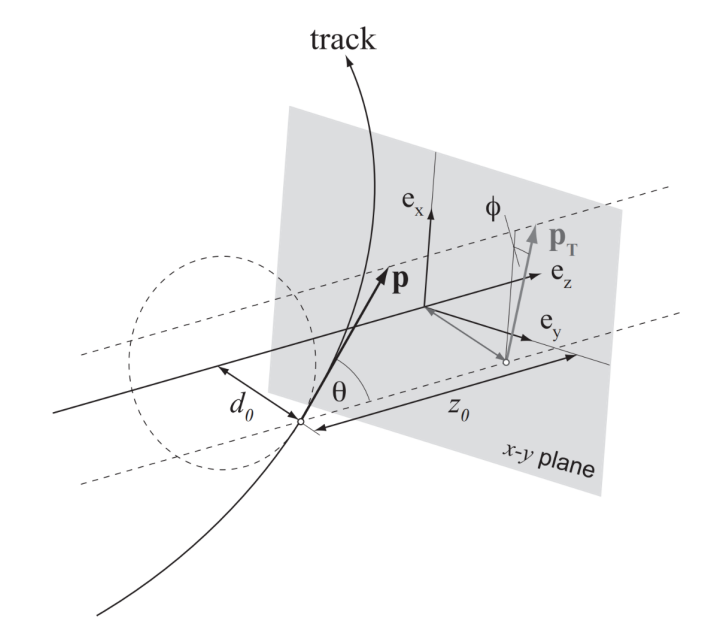
\includegraphics{track_schematic.png}
  \caption{The track parameters defining a helical trajectory.}
  \label{fig:trk_params}
\end{figure}

%% Kalman filter -- dedicated subsection?
A helical track path is defined by the 5-tuple
\( \left( d_0, z_0, \theta, \phi, q/p \right) \)
where $d_0$ and $z_0$ are the transverse and longitudinal distance from the beamspot at the point of closest approach, $\theta$ and $\phi$ are the polar and azimuthal angles of the track at this point, and $q/p$ is the inverse magnitude of the track's total momentum signed by the charge of the particle\footnote{This ratio is related to the transverse radius of curvature $R$ and the axial magnetic field $B$ by $q/p = \sin \theta / B R$.} (\Cref{fig:trk_params}).
However, every interaction with a detector element modifies a charged particle's trajectory through ionization energy loss and multiple scattering.
Since there are tens of hits in most tracks, a typical track has $\mathcal{O}(100)$ parameters in its description, and the parameters before and after a hit are not independent.
It is computationally infeasible to process a single global fit for each track candidate with this many correlated parameters.
A Kalman filter approach is taken instead, which processes a track from one end to the other, updating the parameters and covariance matrix along the way.

The three space-points in a track seed are sufficient to constrain a helical path.
This naive trajectory is used to build a road along which additional silicon hits are checked for.
The Kalman smoother-fitter follows the trajectory and incorporates successive hits into the fit \cite{Cornelissen:2008zza}. %% global chi^2 track fitter
It predicts where hits for a track candidate would be expected in other layers, and a track candidate is penalized if there are no hits near the expected trajectory. %% TODO: more detail on kalman filters?
Under typical LHC circumstances, about 10\% of seeds result in a successful track candidate.

\subsection{Ambiguity solving} %% does this deserve a separate section?

Many of the track candidates at this point have holes, shared hits, or represent fake tracks.
The $\chi^2$ output of the Kalman filter is not a good quantity for determining whether a track is a fake or not\footnote{The $\chi^2$ should follow a corresponding $\chi^2$ distribution, which has a tail that extends to positive infinity. Selecting tracks based on their $\chi^2$ would lead to a biased sample.}.
A track scoring strategy is used that penalizes track candidates for holes using different weights depending on the location of the hole in the detector \cite{Wicke:1998efw}.
In general, measurements from more precise detector systems are given larger weights.
Shared hits from two or more tracks are assigned to the track with the largest score, and the remainder of the tracks with the shared hit are refit neglecting this hit, and their score is re-calculated.
Track candidates with a score that falls below a certain quality threshold are removed, and this process is performed iteratively until the set of tracks remains unchanged.

\subsection{TRT track extension}

The trajectory of each track from the silicon detectors is followed into the \trt, where compatible hits are searched for.
If a possible extension is found, the track is refit and re-scored with the \trt hits.
If the extended track has a higher score than the silicon-only track, then the track is updated with the extension.
Otherwise the original silicon track is kept and the \trt hits are kept as outliers.

\section{Track selection} %% ? does this need its own section? possibly in analysis section

The tracks used for the results in this thesis are inside-out and low-\pt tracks.
Tracks from back-tracking are not used because they are typically secondary particles.
The offline track selection is that used in the \pPb multiplicity analysis \cite{HION-2012-15}, which is based on the \pp \minbias spectra analysis \cite{STDM-2010-06} with some additional cuts on impact parameter ($d_0$ and $z_0$) significance.
\begin{itemize}
\item
  The track must have $\pt \geq 0.1 \GeV$ and $|\eta| < 2.5$.
\item
  A track with $\pt \geq $ 0.1/0.2/0.3 \GeV must have at least 2/4/6 \sct hits.
  These transverse momentum cutoffs correspond approximately to thresholds after which the track is expected to pass through the next \sct layer.
\item
  At least one physical pixel hit is required, and if a B-Layer hit is expected based on the trajectory then there is at least one physical B-Layer hit.
\item
  The transverse and longitudinal impact parameters with respect to the \ac{PV} must satisfy $|d_0^\textrm{PV}| < 1.5 \textrm{ mm}$ and $|z_0^\textrm{PV} \sin\theta| < 1.5 \textrm{ mm}$.
\item
  A significance cut is also placed on the impact parameters such that $|d_0^\textrm{PV}| < 3\sigma_{d_0^\textrm{PV}}$ and $|z_0^\textrm{PV} \sin\theta| < 3\sigma_{z_0^\textrm{PV} \sin\theta}$.
\end{itemize}


\section{Track reconstruction performance}

High-energy \pp and heavy ion collisions are generated with \mc simulations to study the performance of the track reconstruction algorithm.
Proton-lead collision events are generated with \Hijing \cite{Gyulassy:1994ew} and the detector material is simulated with \GEANTFour \cite{Agostinelli:2002hh}.
These simulations are able to provide an accurate description of many track properties, for example the silicon hits per track shown in \Cref{fig:trk_si_hits}.
The efficiency to reconstruct a track in \mc samples is shown in \Cref{fig:trk_eff}.

\begin{figure}[t]
  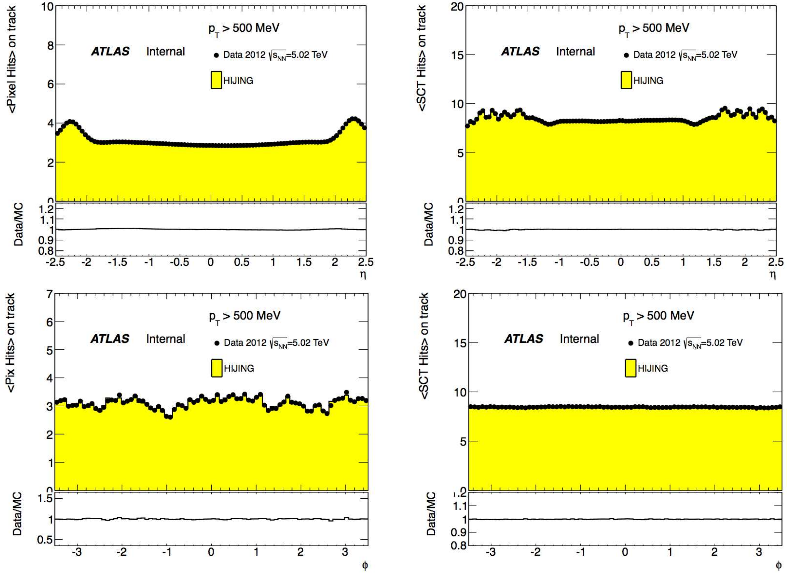
\includegraphics[width=\linewidth]{ATL-COM-PHYS-2013-1017_sihits.png}
  \caption{The mean number of silicon hits on track in Run-1 \pPb collisions as a function of pseudorapidity (top) and azimuthal angle (bottom).}
  \label{fig:trk_si_hits}
\end{figure}

\begin{figure}[t]
  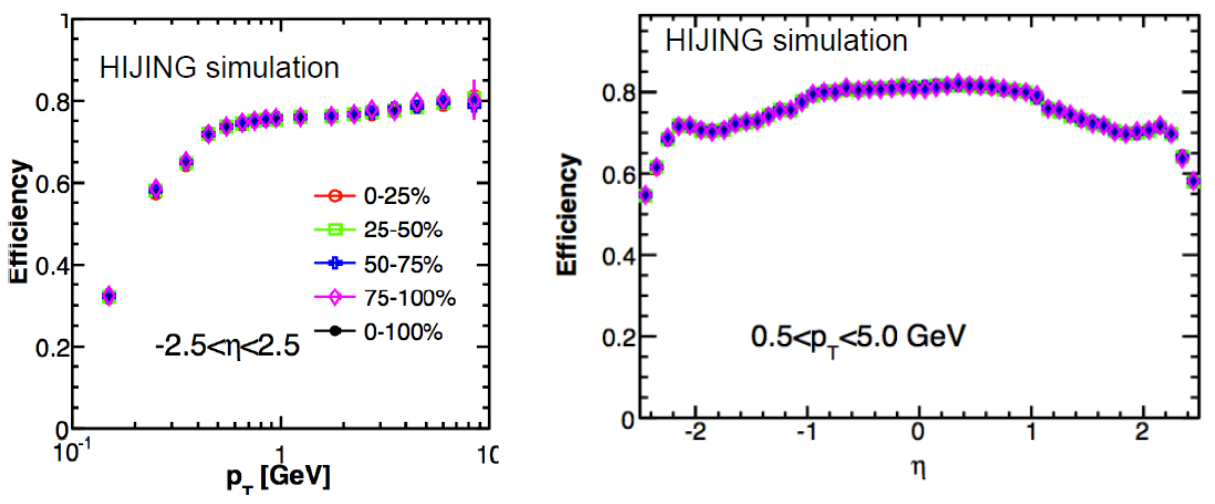
\includegraphics[width=\linewidth]{ATL-COM-PHYS-2013-011_trk_eff.png}
  \caption{The track reconstruction efficiency in Run-1 \pPb collisions as a function of transverse momentum (left) and pseudorapidity (right).}
  \label{fig:trk_eff}
\end{figure}

\section{Pion identification}

\cite{ATLAS-CONF-2011-016}
     % Reconstruction of charged particles
\chapter{Analysis}
\label{ch:analysis}
\graphicspath{{Chapter-Analysis/figures/}}

\section{Data set}

The analyses presented in this thesis use the data from the 2013 \pPb run at the \ac{LHC} with a center-of-mass energy of \pPbenergy for a total integrated luminosity of \pPblumi.
The Pb ions had an energy per nucleon of $1.57 \TeV$ and collided with the $4 \TeV$ proton beam resulting in a net longitudinal boost of the center-of-mass system of $\ycm = 0.465$ in the proton direction relative to the ATLAS laboratory frame.
The \pPb\ run was divided into two periods between which the directions of the proton and lead beams were
reversed. 
The data are presented using the convention that the proton beam travels in the forward ($+z$) direction and the lead beam travels in the backward ($-z$) direction.
When the data from these two periods are combined, the \minbias triggers sampled a total luminosity, after prescale, of $24.5~\mu\textrm{b}^{-1}$ and yielded a total of 44 million events over the full centrality.

For results reported as a function of centrality, an additional \ac{HighET} trigger selection is included in the most central bin that requires the total transverse energy in both sides of the \ac{FCal} to be at least 65 \GeV.
The \ac{HighET} trigger sampled a total luminosity of $41.4~\mu\textrm{b}^{-1}$ after prescale and yielded 700 thousand events to the sample.
Events from this trigger are only included in the 0--1\% centrality interval, where the \ac{HighET} trigger is fully efficient.

Several \acp{HMT} are included to boost the sample used in the azimuthal analysis, with offline \Nch cutoffs at 100, 130, 150, 180, 200, and 225 tracks.
These \acp{HMT} provide a crucial 6.7 million events, as the \minbias triggers provide only 200 000 events at $\Nch > 150$.

All events are required to pass a set of \minbias selection criteria.
Events are required to be included in the latest Good Runs List from ATLAS, which rejects events recorded in conjunction with a technical difficulty in the detector.
The \minbias trigger requires either one hit in both sides of the \ac{MBTS} or two hits in one side.
Additional \ac{HighET} and high multiplicity triggers are included in some analysis bins as discussed above.
%% Events with an offline multiplicity lower than the nominal trigger threshold are excluded, as each of these HMTs reaches an efficiency near 1 near their nominal turn-on. This rejects events that fire a trigger in its turn-on region, as these samples can in principle be biased.
%% In practice no significant difference in the results is observed whether or not events in the HMT triggers' turn-ons are included, so using the nominal turn-on multiplicity is sufficient.
A timing cut is placed on the \ac{MBTS} hits in each side such that $|\Delta t_{AC}| < 10~\textrm{ns}$.
No more than one reconstructed \ac{PV} or strong vertex (where a strong vertex has more than 10 tracks or a total \pt of tracks greater than $6~\GeV$) is permitted in each event.
Diffractive events are identified for rejection by a gap of two units of pseudorapidity in event activity on the Pb-going side of the calorimeters \cite{HION-2012-15}.
Pileup events are also discarded using a run-dependent upper limit on the Pb-going \ac{ZDC}.
In addition, events are discarded if an error flag is recorded in the \ac{LAr} or tile calorimeter systems, or if there is an indication that the event was not completely recorded.

\subsection{Centrality determination}

\begin{figure}[t]
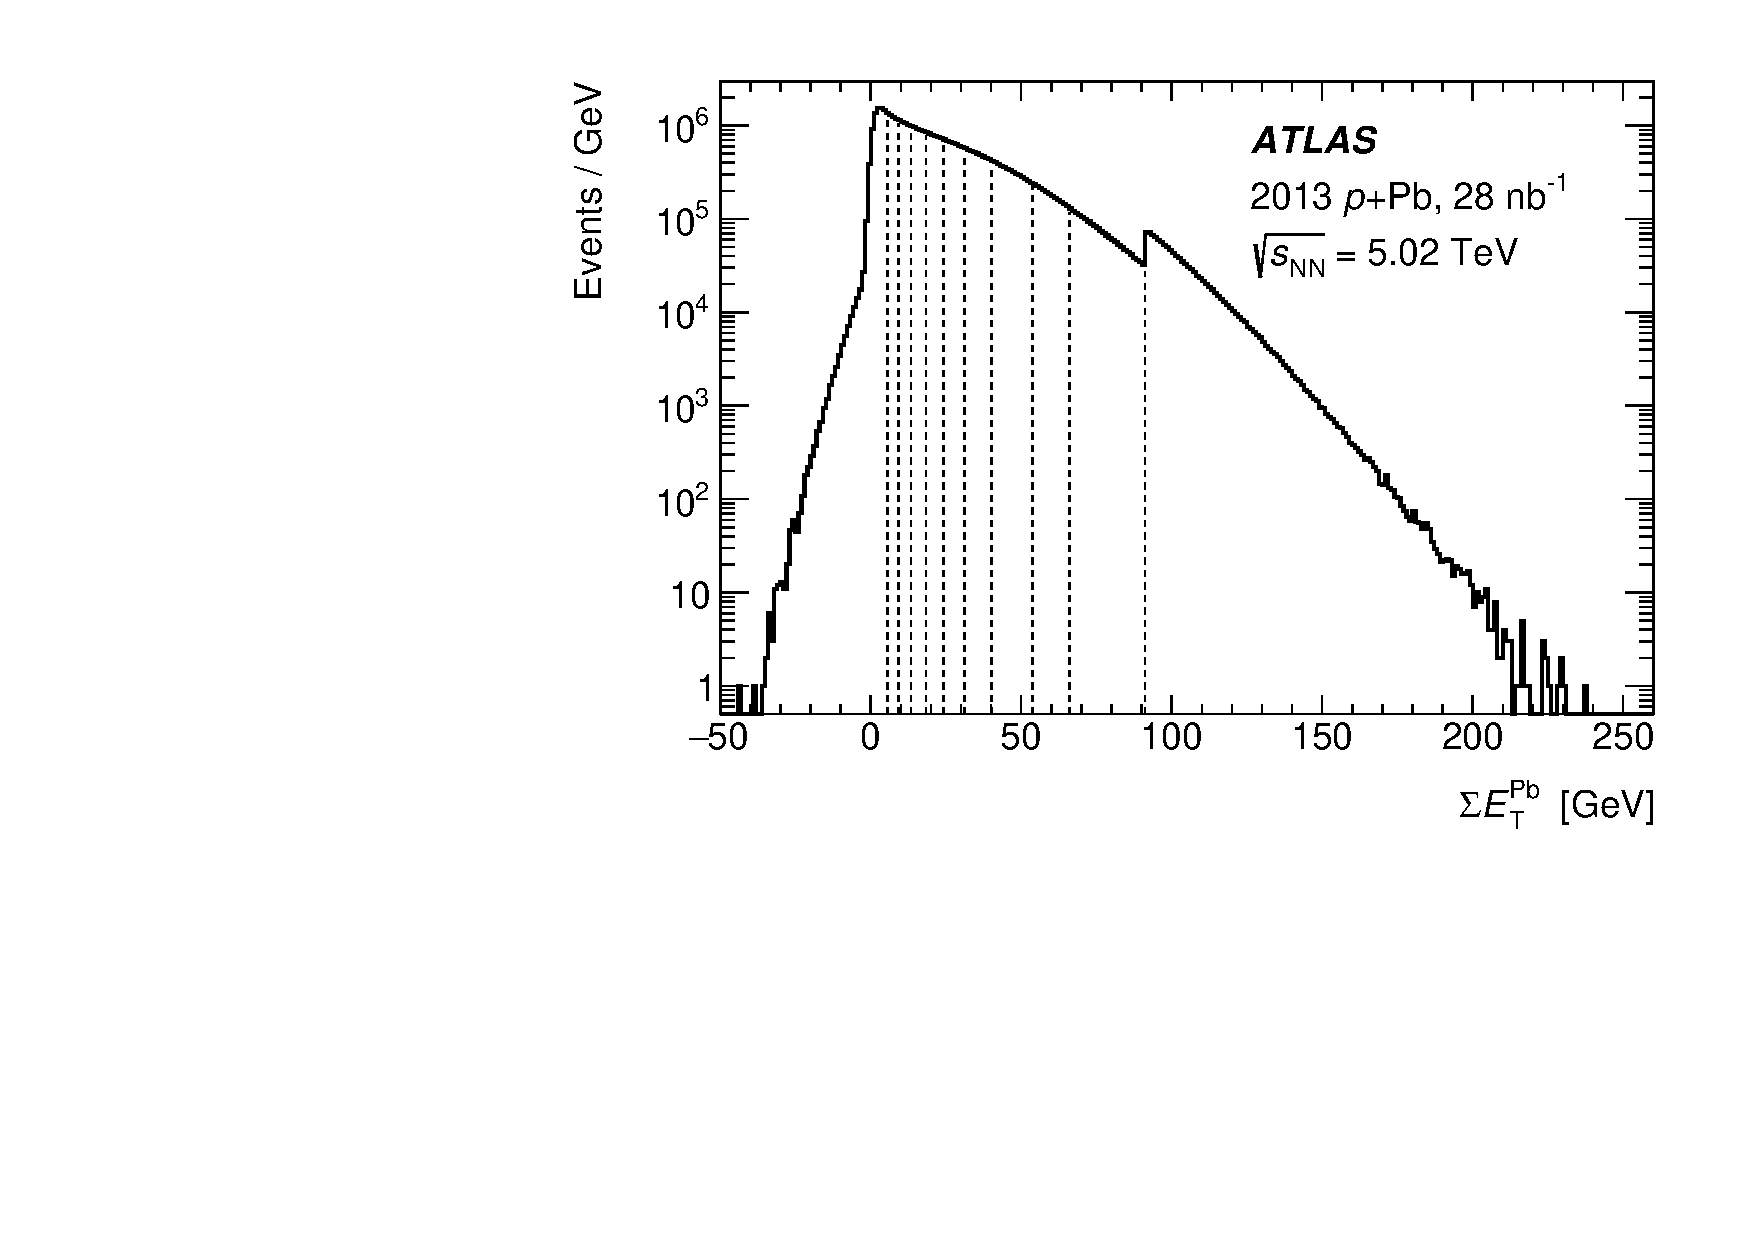
\includegraphics{fcal_et_total.pdf}
\caption{The distribution of the total transverse energy in the \ac{FCal} in the Pb-going direction (\sumETPb) for the events used in the centrality-dependent analysis. Dashed lines are shown at the boundaries of the centrality intervals, and the discontinuity at $\sumETPb = 91.08~\GeV$ corresponds to the lower \sumETPb boundary of the 0--1\% centrality interval.}
\label{fig:fcal_et}
\end{figure}

The centralities of the \pPb\ events are characterized following the procedures described in \Ref{\cite{HION-2012-15}}, using the total transverse energy in the Pb-going side of the \ac{FCal}, \sumETPb.
The use of the \ac{FCal} for measuring centrality has the advantage that it is not sensitive to multiplicity flvuctuations in the kinematic region covered by the inner detector, where the measurements are performed.
Measurements are presented in this paper for the centrality intervals listed in \cref{table:npart}.
The events selected using the \ac{HighET} trigger are used only in the 0--1\% centrality interval.
\cref{fig:fcal_et} shows the distribution of \sumETPb\ values obtained from events included in this
measurement.
The discontinuity in the spectrum occurs at the low edge of the 0--1\% centrality interval, above which the \ac{HighET} events are included.

For each centrality interval, the average multiplicity of charged particles with $\pt > 100~\MeV$ and $|\eta| < 1.5$, \avgdNdeta and the corresponding average number of participating nucleons, \avgNpart, are obtained from a previous publication \cite{HION-2012-15}.
Since this analysis uses finer centrality intervals (no wider than 10\% of the total centrality range) than
those used in \Ref{\cite{HION-2012-15}}, a linear interpolation over the Glauber \avgNpart is used to construct additional values for \avgdNdeta based on the published results.
This interpolation is justified by the result in \Ref{\cite{HION-2012-15}} that charged-particle multiplicity is proportional to \avgNpart in the peripheral region.
The values and uncertainties from this procedure are listed in \cref{table:npart}.


\renewcommand{\arraystretch}{1.1}
\begin{table}
\begin{center}
\begin{tabular}{r || c | c | c || c}
\hline
 & \multicolumn{3}{c||}{\avgNpart} & \\ \cline{2-4}
Centrality & Glauber & GGCF $\omega_{\sigma} = 0.11$ & GGCF $\omega_{\sigma} = 0.2$ & $\avgdNdeta$\\
\hline \hline
0--1\% & $ 18.2^{+2.6}_{-1.0} $ & $ 24.2^{+1.5}_{-2.1} $ & $ 27.4^{+1.6}_{-4.5} $ & $58.1\ \pm 0.1\ \ \pm 1.9\ $ \\[2pt]
\hline
1--5\% & $ 16.10^{+1.66}_{-0.91} $ & $ 19.5^{+1.2}_{-1.3} $ & $ 21.4^{+1.5}_{-2.0} $ & $45.8\ \pm 0.1\ \ \pm 1.3\ $ \\[2pt]
\hline
5--10\% & $ 14.61^{+1.21}_{-0.82} $ & $ 16.5^{+1.0}_{-1.0} $ & $ 17.5^{+1.1}_{-1.1} $ & $38.5\ \pm 0.1\ \ \pm 1.1\ $ \\[2pt]
\hline
10--20\% & $ 13.05^{+0.82}_{-0.73} $ & $ 13.77^{+0.79}_{-0.81} $ & $ 14.11^{+0.86}_{-0.79} $ & $32.34 \pm 0.05 \pm 0.97$ \\[2pt]
\hline
20--30\% & $ 11.37^{+0.65}_{-0.63} $ & $ 11.23^{+0.62}_{-0.67} $ & $ 11.17^{+0.68}_{-0.62} $ & $26.74 \pm 0.04 \pm 0.80$ \\[2pt]
\hline
30--40\% & $ 9.81^{+0.56}_{-0.57} $ & $ 9.22^{+0.50}_{-0.54} $ & $ 8.97^{+0.60}_{-0.49} $ & $22.48 \pm 0.03 \pm 0.75$ \\[2pt]
\hline
40--50\% & $ 8.23^{+0.48}_{-0.55} $ & $ 7.46^{+0.41}_{-0.43} $ & $ 7.15^{+0.54}_{-0.39} $ & $18.79 \pm 0.02 \pm 0.69$ \\[2pt]
\hline
50--60\% & $ 6.64^{+0.41}_{-0.52} $ & $ 5.90^{+0.36}_{-0.34} $ & $ 5.60^{+0.47}_{-0.30} $ & $15.02 \pm 0.02 \pm 0.62$ \\[2pt]
\hline
60--70\% & $ 5.14^{+0.35}_{-0.43} $ & $ 4.56^{+0.32}_{-0.26} $ & $ 4.32^{+0.41}_{-0.23} $ & $11.45 \pm 0.01 \pm 0.56$ \\[2pt]
\hline
70--80\% & $ 3.90^{+0.24}_{-0.30} $ & $ 3.50^{+0.22}_{-0.18} $ & $ 3.34^{+0.29}_{-0.16} $ & $ \ \  8.49 \pm 0.02 \pm 0.51$ \\[2pt]
\hline
\end{tabular}
\caption{The average number of nucleon participants \avgNpart \cite{HION-2012-15} for each centrality interval in the Glauber model as well as the two choices for the Glauber-Gribov model with color fluctuations (GGCF) \cite{Alvioli:2013vk} (and references therein), along with the average multiplicity with $\pt > 100~\MeV$ and $|\eta| < 1.5$ also obtained from Ref.~\cite{HION-2012-15}. The parameter $\omega_{\sigma}$ represents the size of fluctuations in the nucleon-nucleon cross section. Asymmetric systematic uncertainties are shown for \avgNpart. The uncertainties in \avgdNdeta are given in the order of statistical followed by systematic.}
\label{table:npart}
\end{center}
\end{table}

 

\subsection{Multiplicity selection}

\begin{figure}[t]
\centering
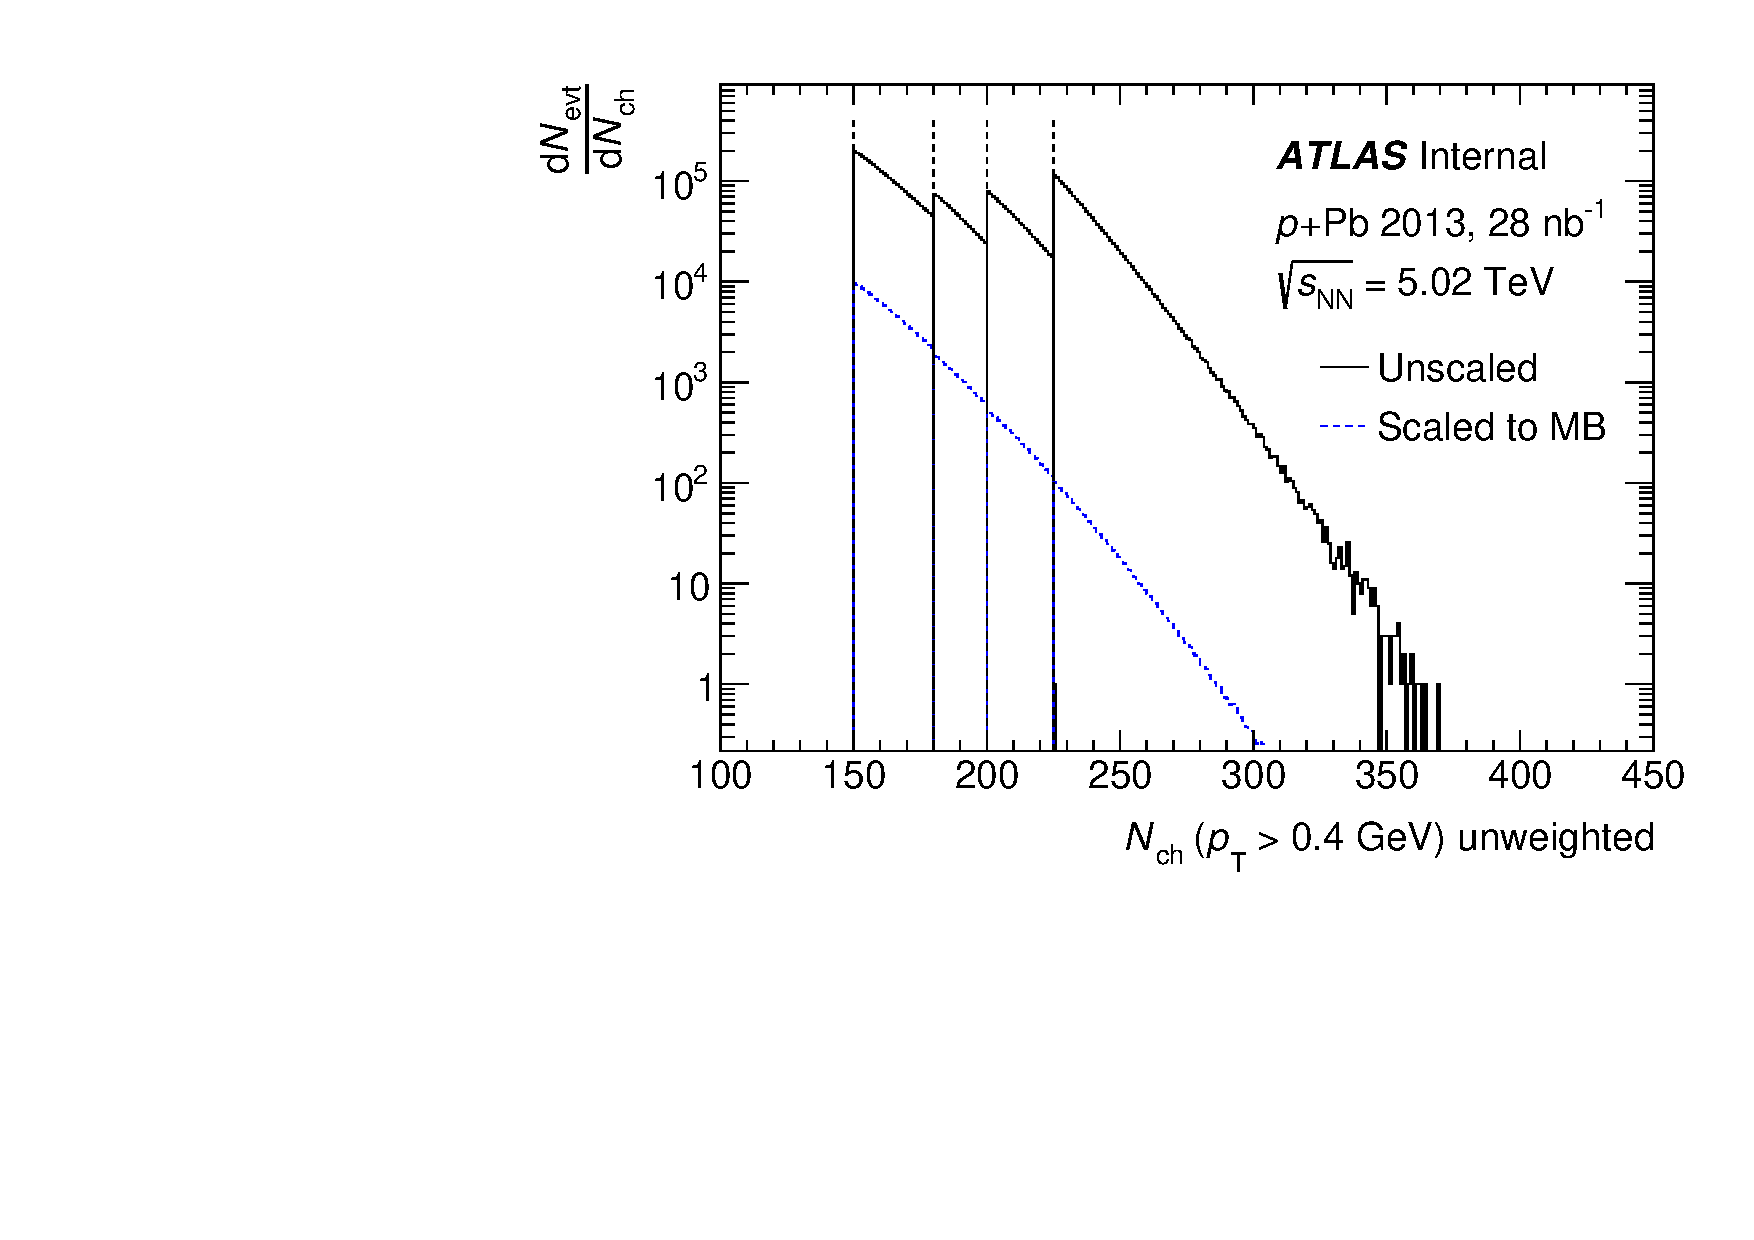
\includegraphics{can_nch.pdf}
\caption{The charged-particle multiplicity \Nch of tracks with $\pt > 0.4$ GeV. Each of the 4 cutoffs corresponds to additional triggers used in the analysis. The distribution scaled down to match the scale of the events from the MinBias trigger is also shown by the dashed blue line.}
\label{fig:nch}
\end{figure}

For the azimuthally-dependent results, events are selected by their reconstructed charged-particle multiplicity \Nch, with a minimum value of 150.
Tracks are only counted towards \Nch if they have $\pt > 400 \MeV$, where the reconstruction efficiency is relatively constant.
This choice permits the straightforward inclusion of several \acp{HMT} into the sample, which is particularly useful because only central events allow a sufficiently high event plane resolution.
The multiplicity distribution is shown in \cref{fig:nch} along with a scaled version to match the \minbias distribution.

%% ---------------------------------
%% event plane determination
%% ---------------------------------
\section{Flow vector determination}

The 2nd-order azimuthal Fourier components $Q_2$ of the energy flow are defined by
\begin{equation}
  Q_2 = \sum_{i}  \et{}_i \begin{pmatrix} \cos 2\phi_i \\ \sin 2\phi_i \end{pmatrix} \; ,\\
\end{equation}
where the sum is taken over calorimeter cells and $\phi_i$ is the ATLAS detector coordinate $\phi$ of the $i$th calorimeter cell.
The two-component elliptic flow vector \qt is defined in terms of $Q_2$, normalized by the 0th-order Fourier component
\begin{equation}
  \qt = \frac{Q_2}{\sum_i \et{}_i } \; .\\
\end{equation}
The elliptic flow used in this analysis is taken from calorimeter cells on the Pb-going side of the detector with $\eta < -2.5$ for period B or $\eta > 2.5$ for period A, which has the beam orientation reversed.
This forward cut is made so as to not overlap with the inner detector.

The second-order event plane angle \psit is defined as
\begin{equation}
2\psit = \mathrm{atan2}(\qt{}_{,y},\qt{}_{,x})
\end{equation}
and is degenerate under $\psit \rightarrow \psit + \pi$.
The magnitude of the flow vector is $|\qt| = \sqrt{\qtx^2 + \qty^2}$; this is essentially a proxy for the total event flow $v_2$ but computed only in the forward region to remove auto-correlations with the inner detector.
An equivalent expression of these equations is
\begin{equation}
\qt = |\qt| e^{i2\psit} = \frac{\sum_i \et{}_i e^{i2\phi_i}}{\sum_i \et{}_i} \; .
\end{equation}
A sketch of the relationship of event plane angle to transverse momentum is shown in \cref{fig:ep_cartoon}.

\begin{figure}[t]
  \centering
  \includegraphics[width=\linewidth]{event_plane_cartoon.png}
  \caption{The event plane angle $\psit$ in relation to the elliptic moment of transverse energy. An exaggerated example of the transverse profile in a hydrodynamic system is shown in blue. The pressure gradients are larger along the axis of narrower extent, leading to greater final momentum in that direction.}
\label{fig:ep_cartoon}
\end{figure}

\subsection{First-order correction}
Due to non-uniformities in the calorimeter response the measurement of the \qt vector can be biased.
This leads to a non-uniform distribution of event plane angle \psit with an additive term proportional to $\cos [2(\psit - \phi_0)]$ which is obviously not physical.
This bias is corrected by subtracting off the mean \qt on a run-by-run basis.
The mean components of the \qt vector are shown in \cref{fig:mean_q2}.
The correction factors are statistically consistent in different multiplicity intervals, so all multiplicities are combined to increase their statistical significance.

\begin{figure}[t]
\centering
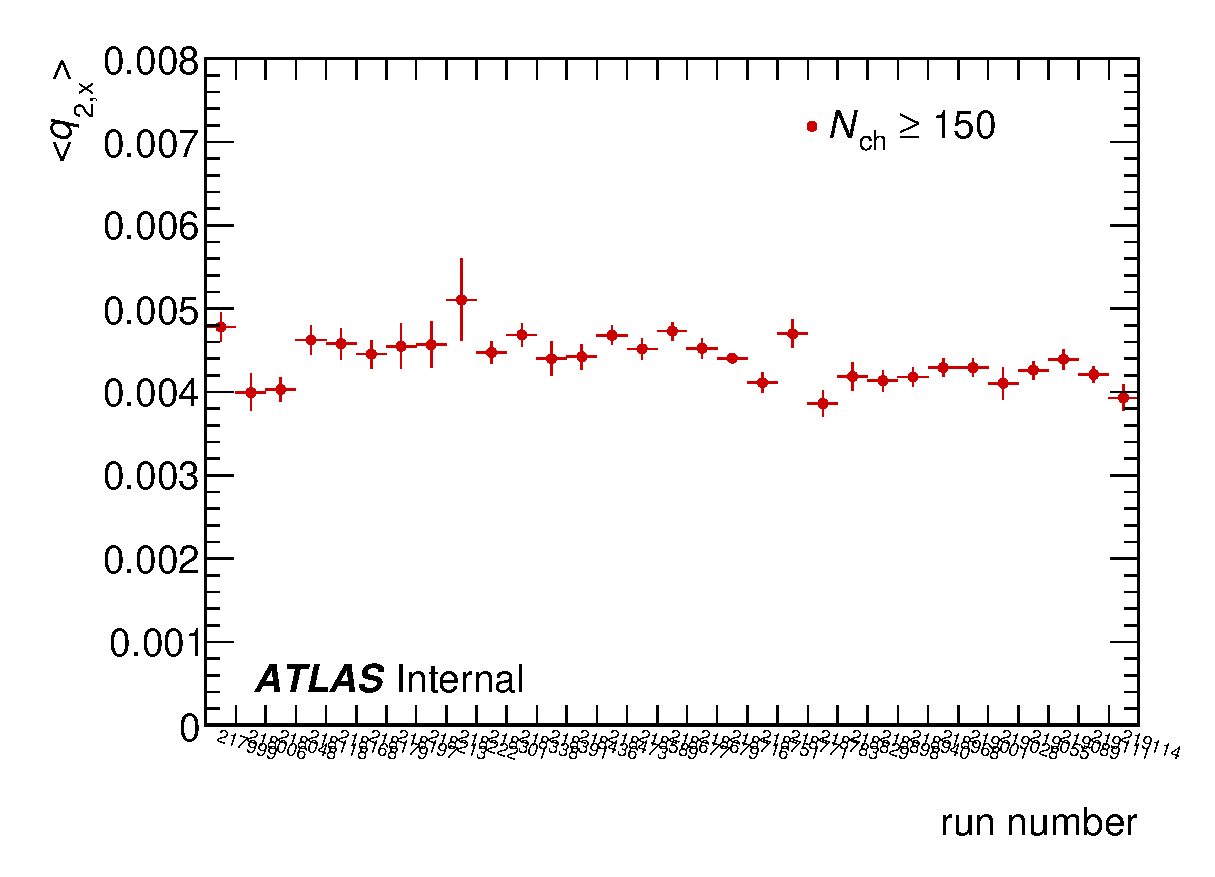
\includegraphics[width=.49\linewidth]{can_qx.eps}
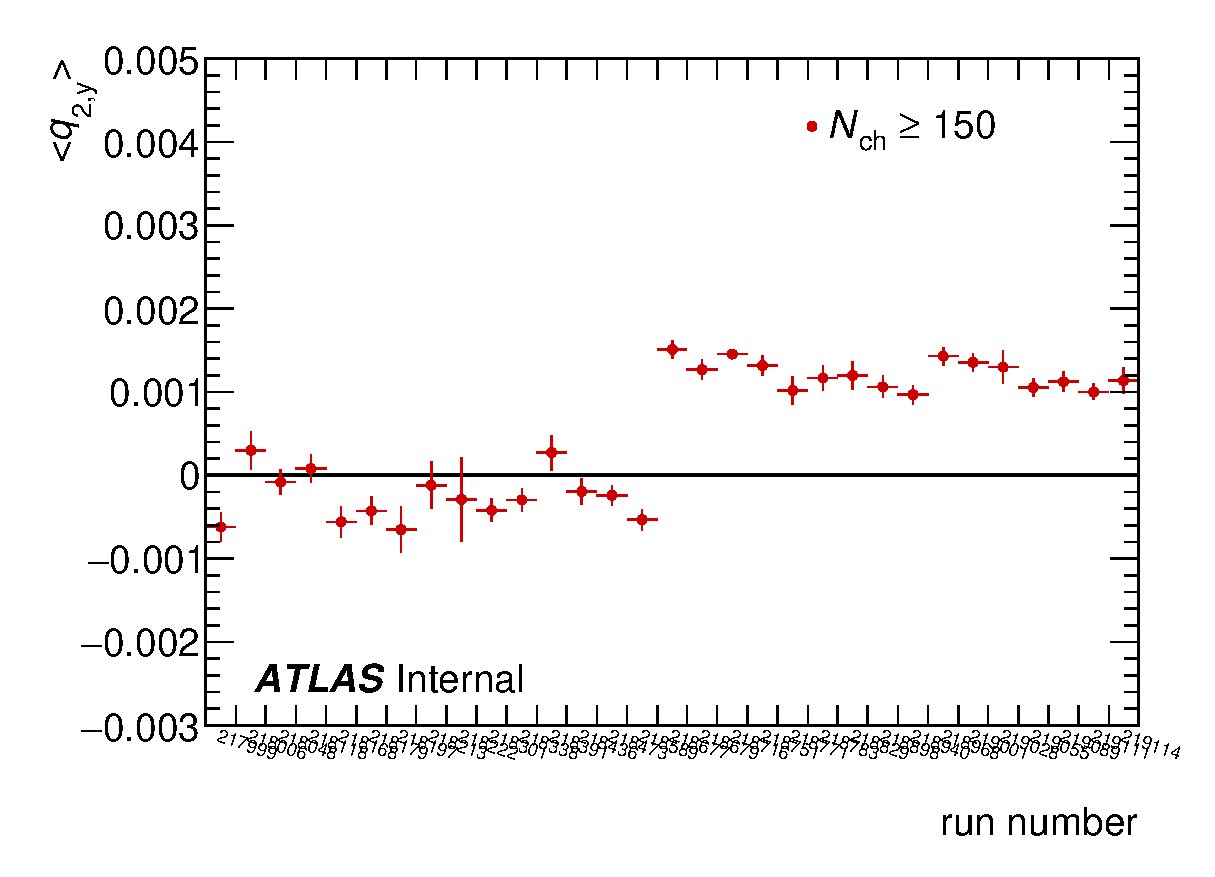
\includegraphics[width=.49\linewidth]{can_qy.eps}
\caption{The average components of the \qt vector $\langle\qtx\rangle$ (left) and $\langle\qty\rangle$ (right) for each run. Runs up to 218589 are from period A, and use $\eta > 2.5$, while runs after this are from period B and use $\eta < -2.5$.}
\label{fig:mean_q2}
\end{figure}

\subsection{Second-order correction}

Some additional non-uniformities persist in the \psit distribution even after correcting for the nonvanishing $\langle\qt\rangle$.
These contribute to higher-order Fourier terms like $\cos (4\psit)$ and $\sin(4\psit)$ in the distribution of the event plane angle \psit.
They arise because detector irregularities can lead to higher-order distortions in the distribution of the matrix of products $\qt{}_i \qt{}_j$.
In order to correct for these and make $\langle \qt{}_i \qt{}_j \rangle$ proportional to the identity matrix the mean-corrected \qt vector is multiplied by the normalized inverse square root of the covariance matrix
\begin{equation}
\frac{1}{\sqrt{N}} \left( \begin{array}{ccc}
  \langle \qty^2 \rangle + D & -\langle\qtx\qty\rangle \\
  -\langle\qtx\qty\rangle & \langle \qtx^2 \rangle + D
  \end{array} \right) \; ,
\end{equation}
where $D = \sqrt{\langle \qtx^2 \rangle \langle \qty^2 \rangle - \langle \qtx \qty \rangle ^2}$ and $N = D\left(\langle \qtx^2 \rangle + \langle\qty^2\rangle + 2D\right)$.
The components of the covariance matrix are shown in \cref{fig:mean_q2_cov}.
This multiplication removes the skew from the \qt distribution and causes it to have the same width in the \qtx and \qty axes.

\begin{figure}[t]
\centering
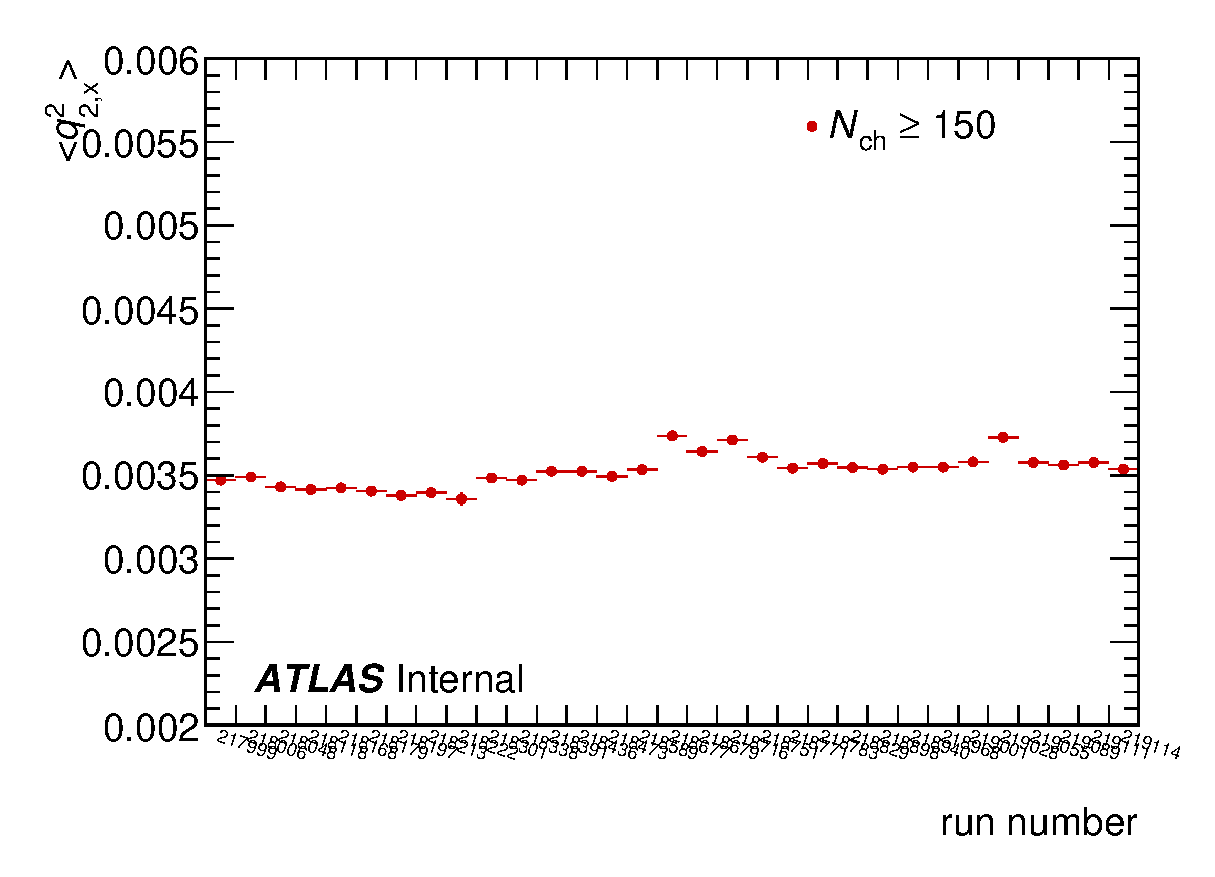
\includegraphics[width=.49\linewidth]{can_qxx.eps}
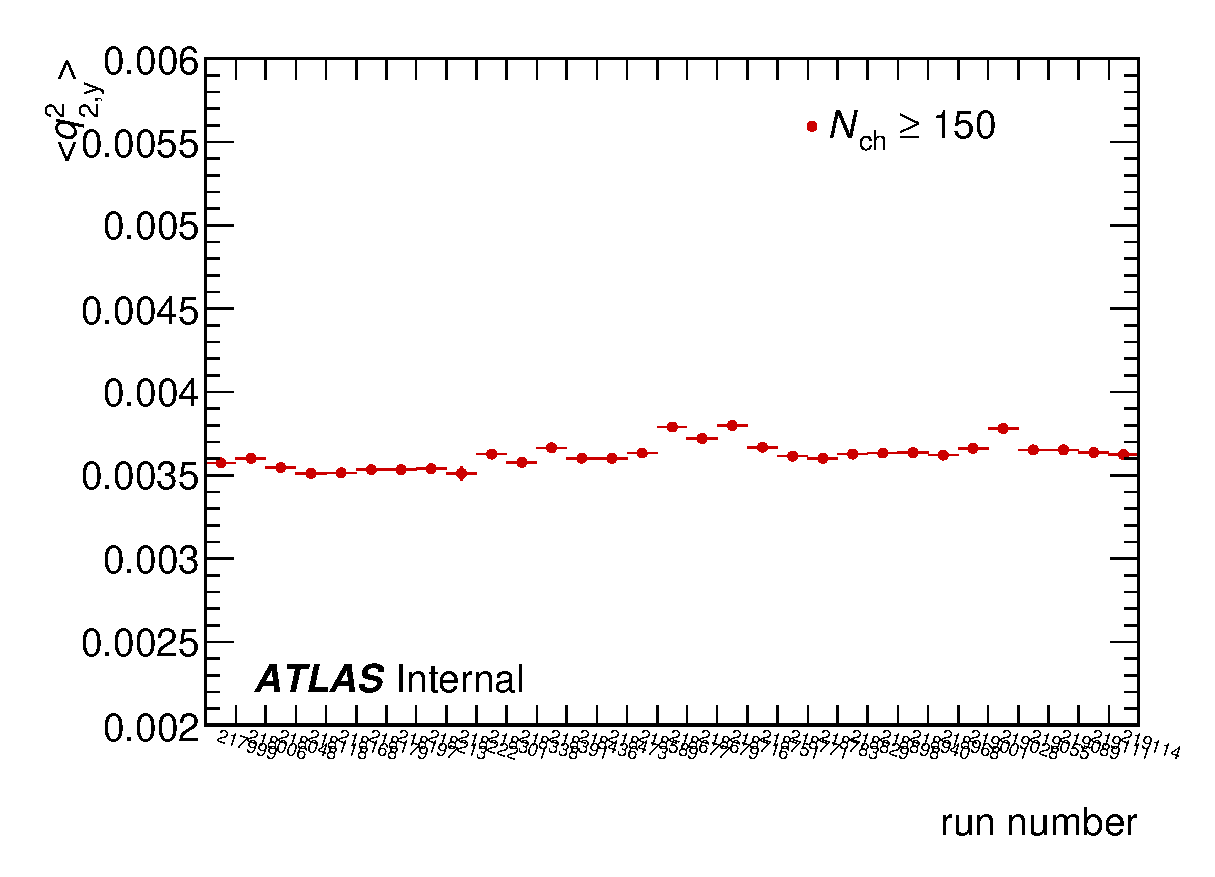
\includegraphics[width=.49\linewidth]{can_qyy.eps}\\
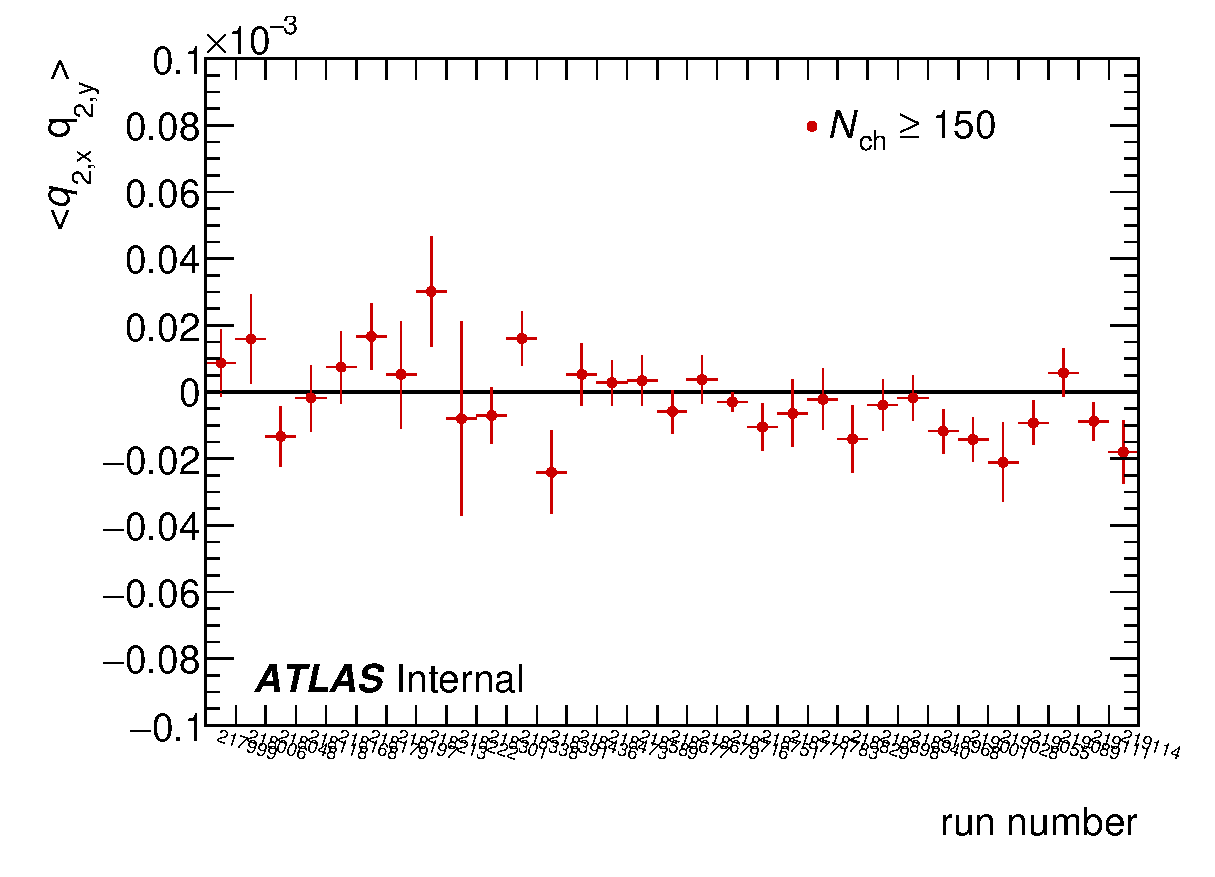
\includegraphics[width=.49\linewidth]{can_qxy.eps}
\caption{The average components of the $<\qt{}_i \qt{}_j>$ matrix for each run. Runs up to 218589 are from period A, and use $\eta > 2.5$, while runs after this are from period B and use $\eta < -2.5$.}
\label{fig:mean_q2_cov}
\end{figure}

As is the case for the mean subtraction correction, the correction factors are consistent over multiplicity so the events are combined for improved statistical significance in the correction.
Once these two corrections are applied run-by-run, the \psit distribution is flat (\cref{fig:dNdpsi2_corr,fig:dNdpsi2_corr_binned}).

\begin{figure}[t]
\centering
\includegraphics{dNdpsi2.eps}\\
\caption{The distribution of second-order event plane angle after first- and second-order flow vector corrections.}
\label{fig:dNdpsi2_corr}
\end{figure}

\begin{figure}[t]
\centering
\includegraphics[width=.49\linewidth]{can_psi2_Nch150to179.png}
\includegraphics[width=.49\linewidth]{can_psi2_Nch180to199.png}
\includegraphics[width=.49\linewidth]{can_psi2_Nch200to224.png}
\includegraphics[width=.49\linewidth]{can_psi2_Nch225.png}
\caption{The distribution of second-order event plane angle, in bins of flow vector magnitude $|\qt|$. Each panel shows a different interval of reconstructed charged particle multiplicity \Nch.}
\label{fig:dNdpsi2_corr_binned}
\end{figure}


\subsection{Event plane angular resolution}
\label{subsec:epres}
\begin{figure}[t]
\centering
\includegraphics{epRes.pdf}\\
\caption{The event plane resolution as a function of the magnitude of the flow vector $|\qt|$ calculated using calorimeter cells with $\eta < -2.5$. Four different intervals of reconstructed track multiplicity \Nch used in the analysis are shown. The systematic uncertainties are shown in the bands, and statistical uncertainties are too small to be visible.}
\label{fig:ep_res}
\end{figure}

The event plane angular resolution, defined as $\langle \cos(2 \delta \psit) \rangle$ where $\delta \psit$ is the difference between true and measured \psit, is shown in \cref{fig:ep_res} measured with the calorimeters in the lead-going direction at $\eta < -2.5$.
The resolution is shown separately for periods A and B, but since they are comparable only the combined resolution is used.
This quantity can be calculated from data using the three-sub-event method, where two other subdetectors are chosen with rapidity ranges $-2 < \eta< -0.5$ and $0 < \eta < 1.5$.
In this expression each subevent is defined by pseudorapidity ranges with a pseudorapidity gap of 0.5 left in between each subdetector so that biases are not introduced from jets overlapping two subdetectors.
The event plane resolution of the nominal subdetector can be calculated with the following expression.
\begin{equation}
\langle \cos(2 \delta \psit) \rangle = \sqrt{ \frac{\langle \cos(2\psit^A - 2\psit) \rangle \langle \cos(2\psit^B - 2\psit) \rangle }{\langle \cos(2\psit^A - 2\psit^B) \rangle} }\\
\end{equation}
Here $\psit^A$ refers to the event plane measured using calorimeters with $-2 < \eta< -0.5$ and $\psit^B$ refers to that with $0 < \eta < 1.5$.
Each of these additional subevents has first- and second-order corrections applied that are derived for each region of the detector in the same way that the corrections are derived for the nominal subdetector with $\eta < -2.5$.
Systematic uncertainties in the event plane resolution are taken from two sources.
The alternate subdetectors are shifted by $\Delta\eta = +0.5$ and the difference in the EP resolution is symmetrized.
Also, the alternate subdetectors are calculated using the \qt from tracks weighted by their \pt.
This difference is also symmetrized, and these two contributions are added in quadrature.


\FloatBarrier
\section{Correlation function}
\label{sec:corr_func}
The two-particle correlation function is defined as the ratio of two-particle to single-particle momentum spectra:
\begin{equation} \label{eq:corr_deff}
  %% ; \kt, \kys, \kphi
  C\left(\mathbf{p}^a, \mathbf{p}^b\right) \equiv \dfrac{\left(\dfrac{dN^{ab}}{d^3\mathbf{p}^a d^3\mathbf{p}^b}\right)}{\left(\dfrac{dN^{a}}{d^3\mathbf{p}^a}\right)\left(\dfrac{dN^{b}}{d^3\mathbf{p}^b}\right)} \,,
\end{equation}
for pairs of particles with momenta $\mathbf{p}^a$ and $\mathbf{p}^b$.
The correlation function is expressed as a function of the relative momentum $\mathbf{q} \equiv \mathbf{p}^a - \mathbf{p}^b$ in intervals of the transverse component \kt of the average momentum $\mathbf{k} \equiv \left(\mathbf{p}^a + \mathbf{p}^b\right)/2$.
The correlation function is measured in intervals of transverse pair momentum \kt and either the rapidity \kys or the azimuthal angle of the pair with respect to the second-order event plane, $\kphi-\psit$.
Because the second-order event plane angle is two-fold degenerate, the observables are invariant under an azimuthal rotation $\kphi \rightarrow \kphi + \pi$, and can be expressed without loss of generality as functions of $\tdpk$. %% \equiv 2(\kphi-\psit)$. %% come up with other notation?
The kinematic variables for the azimuthal analysis are shown in a transverse projection in \Fig{\ref{fig:transverse_q}}.

\begin{figure}[t]
  \centering
  \includegraphics{transverse_q.png}
  \caption{A transverse projection of the kinematic variables of a track pair with respect to the event plane.}
\label{fig:transverse_q}
\end{figure}

The numerator and denominator of \Eqn{\ref{eq:corr_deff}} are expressed in terms of the variables of interest with the following notation:
\begin{align}
  A\left[\mathbf{q};\kt, \kys, \tdpk\right] &\equiv \left. dN_\textrm{pair}/d^3 \mathbf{q} \right|_{\textrm{same}} \\
  B\left[\mathbf{q};\kt, \kys, \tdpk\right] &\equiv \left. dN_\textrm{pair}/d^3 \mathbf{q} \right|_{\textrm{diff}}
\end{align}
where $A(\mathbf{q})$ is a histogram formed with pairs from the same event in each event class and $B(\mathbf{q})$ is a histogram formed with pairs that do not have correlations from being in the same event but are also each drawn from the same event class.
The combinatorial background $B(q) \equiv \left. dN/dq \right|_{\textrm{diff}}$ is constructed either by event mixing or, for the azimuthal analysis, by the pair sampling procedure.
Each of these approaches will be described below.
The ratio of the distributions defines the correlation function:
\begin{equation}
  \label{eq:same_over_mixed}
  C\left[q;\kt, \kys, \tdpk\right] \equiv \frac{A_{\mathbf{k}}(q)}{B_{\mathbf{k}}(q)}
\end{equation}
which in practice is a function either of \kys or \tdpk, not both.

\subsection{Track pair cuts}
All particle pairs are required to have $\left| \Delta \phi \right| < \pi/2$.
Without this cut an enhancement is observed at large relative momentum from di-jets.
While the physics of interest happens at low relative momentum, an enhancement at large relative momentum can affect the asymptotic normalization of the fit functions, which can in turn impact the quality of the fit.

Opposite-sign pairs are rejected if their $\sqrt{s}$ is near one of a few known resonances.
In calculating the invariant mass of each pair, the track masses are assumed to be one of the sets of possible daughter particles (in this case $\pi^{\pm}$ or $K^{\pm}$).
The pair is rejected if their invariant mass is within $20~\MeV$ of the mass of the possible parent particle, except in the case of the $\rho^{0}$, where pairs are rejected if they are within 2 half-widths of $m_{\rho^{0}}$, at $626.2 \MeV < \sqrt{s} < 924.4 \MeV$.
The decays rejected are the following:
\begin{itemize}
\item
  $\rho^{0} \rightarrow \pi^{+} \pi^{-}$
\item
  $K^{0}_{S} \rightarrow \pi^{+} \pi^{-}$
\item
  $\phi(1020) \rightarrow K^{+} K^{-}$
\end{itemize}

\subsection{Event mixing}
\label{subsec:evt_mixing}
The event-mixed background $B(q) \equiv \left. dN/dq \right|_{\textrm{mix}}$ is constructed by selecting one particle from each of two events in the same event class as $A(q)$.
This approach has the useful property that most single-particle efficiency, acceptance, and resolution effects cancel in the ratio.
This event mixing approach is therefore used when possible except in the azimuthally-dependent analysis where it is precluded by the event plane resolution correction.

Each particle in the background fulfills the same selection requirements as those used in the same-event distribution.
Event classes are categorized by centrality so that events are only compared to others with similar multiplicities and momentum distributions.
Events are also sorted by the longitudinal position of the primary vertex $z_\textrm{PV}$ so that the background distribution is constructed with pairs of tracks originating from nearby space points, which is necessary for $B(q)$ to accurately represent the as-installed detector.
The $A(q)$ and $B(q)$ distributions are combined over $z_\textrm{PV}$ intervals in such a way that each of them represents the same $z_\textrm{PV}$ distribution.

\subsection{Event plane resolution correction}
\label{subsec:epres_corr}
The event plane resolution has the effect of reducing the second-order Fourier components of event-by-event observables.
For instance, given true and measured event plane angles $\psit^\textrm{tr}$ and $\psit^\textrm{m}$ with $\psit^\textrm{m} = \psit^\textrm{tr} + \delta\psit$, the relevant Fourier components of an azimuthally-dependent observable $\mathcal{O}$ are
\begin{equation}
  \begin{split}
    \mathcal{O}^\textrm{m} \left[2(\phi-\psit^\textrm{m})\right] =& \mathcal{O}_\textrm{,0} + \mathcal{O}_\textrm{,c2} \cos\left[2(\phi - \psit^\textrm{m})\right]
    + \mathcal{O}_\textrm{,s2} \sin\left[2(\phi - \psit^\textrm{m})\right]\\
    =& \mathcal{O}_\textrm{,0} + \mathcal{O}_\textrm{,c2} \cos\left[2(\phi - \psit^\textrm{tr} - \delta\psit)\right]
    + \mathcal{O}_\textrm{,s2} \sin\left[2(\phi - \psit^\textrm{tr} - \delta\psit)\right]\\
    =& \mathcal{O}_\textrm{,0} + \left\{\mathcal{O}_\textrm{,c2} \cos\left[2(\phi - \psit^\textrm{tr})\right]
    + \mathcal{O}_\textrm{,s2} \sin\left[2(\phi - \psit^\textrm{tr})\right]\right\} \cos(2\delta\psit)
  \end{split}
\end{equation}
where $\mathcal{O}_\textrm{,0}$ is the 0th-order Fourier component and $\mathcal{O}_\textrm{,c2}$ and $\mathcal{O}_\textrm{,s2}$ are the 2nd-order cosine and sine Fourier components, respectively.
Therefore, over many events the event plane resolution effectively reduces the 2nd-order Fourier components of an observable by a factor of $\langle \cos\left(2\delta\psit\right) \rangle$.
A correction is performed on the same-event distribution $A$, as described in \Ref{\cite{Heinz:2002au}}, to compensate for this effect as well as the effect of non-infinitesimal azimuthal bin widths:
\begin{equation}
  \label{eq:a_corr}
  A^\textrm{corr}[q,\tdpk] = A^\textrm{exp}(q) + 2\xi \left\{ A_\textrm{,c2}(q) \cos\left[\tdpk\right] + A_\textrm{,s2}(q) \sin\left[\tdpk\right] \right\}
\end{equation}
where
\begin{align}
  \xi =& \frac{\pi/N_\textrm{bins}}{\langle \cos\left(2\delta\psit\right) \rangle \sin\left(\pi/N_\textrm{bins}\right)} - 1 \label{eq:xi_def} \\
  A_{,\textrm{c}2}(q) =& \frac{1}{N_\textrm{bins}} \sum_{i=1}^{N_\textrm{bins}} A^\textrm{exp}\left[q,\tdpk_i \right] \cos \left[ \tdpk_i \right] \\ 
  A_{,\textrm{s}2}(q) =& \frac{1}{N_\textrm{bins}} \sum_{i=1}^{N_\textrm{bins}} A^\textrm{exp}\left[q,\tdpk_i \right] \sin \left[ \tdpk_i \right]
\end{align}
and $\Nbins = 8$ is the number of azimuthal bins.
Only the 2nd harmonic is corrected in this procedure. Higher-order harmonics, while potentially of physical interest, are more difficult to measure and are not considered in this analysis.

The combinatoric background $B(q) \equiv \left. dN/dq \right|_{\textrm{mix}}$ is traditionally constructed by event mixing, that is, by selecting one particle from each of two events in the same event class as $A(q)$ as described in \cref{subsec:evt_mixing}.
However, with an azimuthally-differential analysis the event plane resolution correction precludes event mixing because there is no simple decomposition of a mixed-event distribution into its Fourier components (as there are two independent event planes in each event pair).
Previous azimuthal femtoscopic measurements have corrected the mixed-event distribution $B$ in the same way that the same-event distribution $A$ is corrected, as suggested in \Ref{\cite{Heinz:2002au}}.
However, this neglects to account for the fact that the independent smearing of the two event planes changes the shape of the pair distribution, and when projected into $q$-space it cannot be simply corrected bin-by-bin.

On the other hand it is possible to correct the single-particle momentum distribution in the same way as \cref{eq:a_corr}.
The dependent variables are \pt and $\eta$ instead of $\mathbf{q}$, and there are many more azimuthal bins (in \Eqn{\ref{eq:xi_def}} the $N_\textrm{bins} = 64$ of $2(\phi - \psit)$ as opposed to 8 bins of $2(\kphi - \psit)$), but the procedure is otherwise identical.
Pairs of momentum are then sampled from this corrected distribution as discussed in detail in \cref{subsec:bkgd_sampling}.

The correlation function $C(q)$ is then formed by taking the ratio of the corrected same- and mixed-event relative momentum distributions
\begin{equation}
  C(q) = \frac{A^\textrm{corr}(q)}{B^\textrm{corr}(q)}
\end{equation}
where $B^\textrm{corr}$ is generated by sampling pairs from $N^\textrm{corr}$, as described in the following sections.

\subsection{Pair sampling}
\label{subsec:bkgd_sampling}
The single-particle distribution can be corrected for the event plane resolution, following the procedure for the pair distribution.
It is not possible to correct the mixed-event pair distributions properly, at least not without extending the analysis in an additional dimension (\psit) which would require an infeasible amount of memory and CPU resources.
Pairs can be sampled from the single-particle distribution after it is corrected.
Building a background with sampling is usually not as precise as mixed-event distributions, but in an azimuthal analysis the event plane resolution correction is a dominant effect, so it is necessary to structure the measurement around it.

The sampling method does not account exactly for variations of the detector acceptance and efficiency over \pt, $\eta$, and \kphi, because each track contributes a count to a bin which represents a small range of possible values of \pt, $\eta$, and \tdpk.
The sampled background pair distribution $B(q)$ is multiplied by the ratio of an event-mixed distribution to a sampled pair distribution (\cref{fig:sample_to_mix_ratio}) in order to compensate for the effect of the sampling procedure.
Both distributions in this ratio are not corrected for event plane resolution, since such a correction cannot be applied to the mixed-event pair distribution.
At small relative momentum, where the HBT signal is relevant, there is no significant effect from the sampling.
This multiplicative correction is applied as a function of \kt.

It is prohibitive statistically and/or computationally to bin the analysis in \psit as well as \tdpk, which would require increasing the size of the analysis by about a factor of 64.
As a result, the sampled momentum $\mathbf{p}$ distribution does not fully account for azimuthal anisotropies in the pair response of the detector.
This effect is described by the ratio of a distribution of mixed events to a similar distribution in which one of the events is smeared by a random angle (\cref{fig:phi_corr_to_uncorr_ratio}).
The background is multiplied by this ratio, which is evaluated as a function of \kt.

\begin{figure}[t]
\centering
\includegraphics[width=.49\linewidth]{sample_to_mix_ratio_kt0.pdf}
\includegraphics[width=.49\linewidth]{sample_to_mix_ratio_kt3.pdf}\\
\caption{The ratio of a sampled distribution to an event-mixed distribution, both of which are not corrected for event plane resolution. This shows the effect of sampling from a finite number of bins. The central points are shown as circles with statistical uncertainties and the bands indicate the systematic uncertainty, which is discussed in \cref{sec:systematics}.}
\label{fig:sample_to_mix_ratio}
\end{figure}

\begin{figure}[t]
\centering
\includegraphics[width=.49\linewidth]{phi_corr_to_uncorr_ratio_kt0.pdf}
\includegraphics[width=.49\linewidth]{phi_corr_to_uncorr_ratio_kt3.pdf}\\
\caption{The ratio of an event-mixed distribution to an event-mixed distribution with randomized azimuthal angle between the events. This demonstrates the effect of not binning events in \psit. The central points are shown as circles with statistical uncertainties and the bands indicate the systematic uncertainty, which is discussed in \cref{sec:systematics}.}
\label{fig:phi_corr_to_uncorr_ratio}
\end{figure}

The single-particle experimental distribution $N^\mathrm{exp}(\pt, \eta, \tdpp)$ is corrected similarly to the pair distribution $A(q)$ (\cref{eq:a_corr}), however it is also explicitly symmetrized in $\phi$ so there is no sine term added.
\begin{equation}
  \label{eq:n_corr}
  N^\textrm{corr}[\pt, \eta, \tdpp] = N^\textrm{exp}_\textrm{symm}\left[\pt, \eta, \tdpp\right] + 2\xi N_\textrm{,c2}(\pt, \eta) \cos\left[\tdpp\right]
\end{equation}
where
\begin{equation}
N^\textrm{exp}_\textrm{symm}\left[\pt, \eta, \tdpp\right] \equiv \frac{N^\textrm{exp}[\pt, \eta, \tdpp] + N^\textrm{exp}[\pt, \eta, -\tdpp]}{2}  \; .
\end{equation}
Without the explicit symmetrization, fluctuations in the azimuthally-odd part of the distribution can lead to nonphysical sine terms in the sampled background. %% Note that there is no detector effect to consider here: the event plane \psit is effectively integrated over. Detector effects not accounted for as a result of this are considered in a systematic uncertainty.

Events are grouped by run period, $z_\textrm{vtx}$, charged-particle multiplicity \Nch (with $\pt > 400$ \MeV), and flow vector magnitude $|\qt|$, for a total number of classes of $2 \times 40 \times 4 \times 5 = 1600$.
The events are combined within each run period, so that the 15 runs from period A and the 16 runs from period B are combined.
This is necessary to sufficiently populate the single-particle distributions to minimize auto-correlations.
Because the 3D momentum histograms need to be densely populated, a large number of events are needed even when each event has a large multiplicity.
The number of events in each of these event classes is shown in \cref{fig:evt_class}.
Each event class has a minimum of 100 events, but most have greater than 1000.

\begin{figure}[t]
\centering
\includegraphics{evt_class.eps}\\
\caption{Differential probability distribution of the number of event classes having a given number of events, where the event class is determined by run period, $z_\textrm{vtx}$, multiplicity, and flow vector magnitude $|\qt|$. The distribution is normalized to unity.}
\label{fig:evt_class}
\end{figure}

Within each event class, tracks are sampled from the histogram of the single-particle distribution $N \left( \pt, \eta, 2(\phi-\psit) \right) $.
A pre-processing step is performed to surjectively assign each bin of the 3D histogram an interval in $(0,1)$ with size proportional to the bin content, representing the cumulative distribution function (CDF) of the histogram distribution at each bin edge.
For each new track a random number is generated in the uniform distribution $U(0,1)$, and a bin is selected by binary search according to the assignment from the pre-processing step.
The values of the three kinematic variables are set by generating uniform random variables from a range of each of the corresponding bin edges.
One of these three random number generations is optimized away, because given that a bin has been selected by the initial random number, that number has a distribution $U(a, b)$ where $a$ and $b$ are the endpoints of its CDF interval.
It can then be scaled linearly to lie between the bin edges of the relevant kinematic variable.
%% with a linear scaling of the value of the initial uniform random number relative to the endpoints of the histogram bin's CDF interval. %% paragraph break?

When pairs tracks are drawn from the same distribution (i.e. same-charge particles in an event class), an additional step is taken to simulate sampling without replacement.
If the second track is randomly drawn from the same bin as the first track, the process continues as normal only with probability $\frac{N_\textrm{bin count} - 1}{N_\textrm{bin count}}$.
In other words, the bin is rejected with probability $1/N_\textrm{bin count}$.
Otherwise the bin is disallowed for the second particle, and its bin is redrawn until it corresponds to a different bin than the first particle's.
Without this correction for sampling-without-replacement, there is a small but significant enhancement at low $|\mathbf{q}|$ of the sampled pair distribution relative to the classically event-mixed distribution.

\begin{figure}[t]
\centering
\includegraphics[width=.49\linewidth]{pos_pt.png}
\includegraphics[width=.49\linewidth]{pos_pt_zoom_bin.png}\\
\caption{The \pt spectrum for positive tracks (left), and a zoomed view of the low-\pt region (right). Each segment is fit to a gamma distribution with variable location which represents the smooth spectrum. The segments are determined by edges at 100, 200, 300, and 400 \MeV, where there are jumps in SCT hit requirements or a turn-on of TRT seeding (at 400 \MeV).}
\label{fig:pt_fits}
\end{figure}

\FloatBarrier

The physical \pt distribution has a steep slope in many places, and the detector response is relatively smooth as a function of \pt.
By contrast, the sampled distribution from the histogram of the single-particle distribution will have sharp jumps at bin edges, so where the slope is large the value of the sampling distribution can be far from that of a smooth one near a bin edge (see \cref{fig:sample_slope_corr}, right).
A correction procedure is applied to remove these sharp edges in the \pt profile of the sampled distribution. In each event class, the \pt distribution is fit to a 4-parameter gamma distribution in four intervals (with boundaries corresponding to changes in the \sct hit requirements).
A first-order correction is performed to transform the a random \pt value to another one in the same bin, to account for the slope of the probability distribution in that bin.
The slope used for this procedure is that computed from the fit function in the \pt interval.
The adjusted \pt is given by
\begin{equation}
  \pt \rightarrow \pt + \frac{f'}{2} (b-a) (\pt-a) (b-\pt)
\end{equation}
where the bin edges of the \pt bin are $a$ and $b$ and the approximate numeric derivative of the probability distribution is $f'$.
The result of this process is illustrated in \cref{fig:sample_slope_corr} on a toy distribution.
Samples are drawn from a course-binned distribution, and the distribution of the modified random variable accounts for the underlying slope.

\begin{figure}[htb]
\centering
\includegraphics[width=.49\linewidth]{testMomHistSampler.png}
\includegraphics[width=.49\linewidth]{testMomHistSamplerZoom.png}\\
\caption{An illustration of the effects of the \pt slope correction on the sampled momentum distribution. The course-binned histogram is used to generate samples for the fine-binned histogram.}
\label{fig:sample_slope_corr}
\end{figure}


\subsection{Parameterization of the correlation function}

The Bose-Einstein enhancement in the invariant correlation functions is fit to an exponential form:
\begin{equation} C_{\textrm{BE}}(\qinv) = 1 + \mathrm{e}^{- \Rinv \qinv } \,, \label{eq:cbe_qinv}\end{equation}
where \Rinv is the Lorentz-invariant HBT radius. This function corresponds to an underlying Breit-Wigner source density.

The Bose-Einstein component of the three-dimensional correlation functions is fit to a function of the form
\begin{equation}
C_{\textrm{BE}}(\mathbf{q}) = 1 + \mathrm{e}^{- \left\| R \mathbf{q} \right\|} \;, \label{eq:cbe_qosl}
\end{equation}
where $R$ is the symmetric matrix in \cref{eq:r_matrix_full}.

The full form of the invariant-correlation-function fit to like-charge track pair data including the hard-process background description is
\begin{equation}
C(q) = \mathcal{N} \left[1-\lambda + \lambda K(\qinv)C_{\textrm{BE}}(q)\right] \Omega(q) \,,\label{eq:correlation_function_full}
\end{equation}
where $\mathcal{N}$ is a normalization factor, $C_\mathrm{BE}(q)$ is given by \cref{eq:cbe_qinv} or \cref{eq:cbe_qosl}, the Coulomb correction $K(\qinv)$ is discussed in \cref{subsec:coulomb}, and the hard process background $\Omega(q)$ is discussed in detail in \cref{sec:jet_frag}.
When opposite-charge pairs are fit to constrain the jet fragmentation background, the same expression is used but the sign of the Bohr radius in $K(\qinv)$ is flipped and the Bose-Einstein correlation vanishes such that $C_\mathrm{BE}(q) = 1$.

%% As discussed in \Sect{\ref{subsec:hard_process}}, the opposite-charge correlation functions are fit in the regions where \qinv (or $|\mathbf{q}|$ in 3D) is greater than 100~\MeV. The opposite-charge parameters are highly insensitive to the choice of cutoff, as the $q$ distributions contribute more statistical weight at larger $q$. The same-charge correlation functions are fit in the regions $\qinv > 30~\MeV$ for the invariant fits and $|\mathbf{q}| > 25~\MeV$ in three dimensions.

\subsection{Coulomb correction}
\label{subsec:coulomb}
The residual strong force between charged pions is subdominant to the Coulomb effect and can be neglected in final-state effects \cite{Lednicky:2005tb}.
In heavy ion collisions the Bohr radius of a pair of pions ($a_{\pi} = 387.5 \textrm{ fm}$) is significantly larger than the source size, which is on the order of a few fermi.
The nonrelativistic limit is appropriate since in the region of interest the pions have low relative momentum.
In the limit where the pions come from a point source, their outgoing wavefunction squared is given by the Gamow factor

\begin{equation} \frac{\left| \psi (q, r=0) \right|^2}{\left| \psi (q, r\rightarrow\infty) \right|^2} = G(\qinv) \equiv \frac{4\pi}{a \qinv}\frac{1}{e^{\frac{4\pi}{a \qinv}} - 1} \end{equation}

where $a$ is the Bohr radius\footnote{The literature contains various conventions for the factors of 2.
Here the Bohr radius contains the reduced mass and this definition of $q$ has no factor of $1/2$.}.
For opposite-charged pairs the correction can be applied by taking $a \to -a$, as this effectively flips the sign of the coupling constant $\alpha_{EM}$.

For a source that has a non-zero spatial extent, a correction to this expression is required.
For a spherical Gaussian source of effective size \Reff, the formula for a more precise correction factor $K(\qinv)$ is expressed in terms of a generalized hypergeometric function ${}_2 F_2$ \cite{Maj:2009ue}.
\begin{equation}
  K(\qinv) = G(\qinv) \left[ 1 + \frac{8\Reff}{\sqrt{\pi}a} {}_2 F_2 \left( \frac{1}{2}, 1; \frac{3}{2}, \frac{3}{2}; -\Reff^2 \qinv^2 \right) \right]
\end{equation}
The analytic gradient of the correlation function parameterization is used in the fitting algorithm, so the derivative with respect to \Reff is also required:
\begin{equation}
  \frac{\partial K(\qinv)}{\partial \Reff} = G(\qinv) \frac{8}{\sqrt{\pi}a} {}_1 F_1 \left( 1; \frac{3}{2}; -\Reff^2 \qinv^2 \right) \; .
\end{equation}
The effective size \Reff described here cannot be connected \emph{a priori} to the HBT radii without additional model-dependent assumptions.
It is taken to be proportional to \Rinv with the constant of proportionality adjusted as a systematic variation.

Software implementations of ${}_2F_2 (a_1, a_2; b_1, b_2; z)$ are not generally available.
%% Series approximations for this function are produced here at small and large negative $z$ (used with a cutoff around $z \approx -18$), respectively.
A series expansion around small $z$ follows direction from the definition.
\begin{equation} {}_2F_2 \left( \frac{1}{2}, 1; \frac{3}{2}, \frac{3}{2}; z \right) = \sum_{n=0}^{\infty} \frac{z^n}{(2n+1) \left(\frac{3}{2}\right)_n} \end{equation}
The Pochhammer symbol $(a)_n$ is used to denote the rising factorial \((a)_n \equiv a(a+1)...(a+n-1) = \frac{\Gamma(a+n)}{\Gamma(a)} \).
An asymptotic expansion around $z \to - \infty$ can be derived.
\begin{equation} {}_2F_2 \left( \frac{1}{2}, 1; \frac{3}{2}, \frac{3}{2}; z \right) \approx \frac{\pi^{3/2}}{4\sqrt{-z}} - \sum_{n=1}^{n < |z| + 3/2} \frac{(2n-3)!!}{(2n-1) 2^n |z|^n}  \end{equation}
This expression is a formally divergent asymptotic series for large negative $z$, so the cutoff is chosen after the smallest term.
In practice it agrees to within several digits of precision relatively quickly.

Corresponding expressions for the confluent hypergeometric function appearing in the derivative are given by
\begin{equation}
 {}_1F_1 \left( 1;\frac{3}{2}; z \right) = \sum_{n=0}^{\infty} \frac{z^n}{\left(\frac{3}{2}\right)_n} 
\end{equation}
\begin{equation}
  {}_1F_1 \left( 1; \frac{3}{2}; z \right) \approx \sum_{n=1}^{n < |z| + 3/2} \frac{(2n-3)!!}{2^n |z|^n} \; \textrm{for } z \rightarrow -\infty\;.
\end{equation}

To apply the Coulomb correction in 3D out-side-long coordinates, the average \kt in each bin is used to contract compute \qinv from $\mathbf{q}$.
The following expression takes advantage of working in the \ac{LCMF} so that $k_L = 0$.
\begin{equation}
\qinv^2 = |\mathbf{q}|^2 - \Gamma^2 + \sqrt{\Gamma^4 - 4 |\mathbf{k}_\mathrm{T}|^2 \qout^2} \label{eq:q3_to_qinv}
\end{equation}
where
\begin{equation}
\Gamma^2 = 2 m_{\pi}^2 + 2 |\mathbf{k}_\mathrm{T}|^2 + \frac{1}{2}|\mathbf{q}|^2 \; .
\end{equation}


%% ------------------------------------------
%% Fit procedure
%% ------------------------------------------

\subsection{Fitting the correlation function}

For histograms representing the same-event distribution $A(q)$ and mixed-event distribution $B(q)$, the goal is to somehow pick the best choice for the parameters of $C(q)$ such that $A \sim B C$.
When fitting to histograms that have bins with possibly small statistics, a simple $\chi^2$ minimization may not be sufficient and a log likelihood ratio $\ln\mathcal{L}$ must be maximized \cite{Baker:1983tu}.
A likelihood for the correlation function can be derived by assuming a flat Bayesian prior in the means for Poisson distributed $A$ and $B$, $\mu$ and $\nu$ \cite{Soltz:1994PhDT}:

\begin{equation}
  \begin{split}
    L(C|A,B) &= \iint d\mu \, d\nu \, P(A|\mu) P(B|\nu) \, \delta\left(C - \frac{\mu}{\nu} \right)\\
    &= \iint d\mu \, d\nu \, \frac{\mu^{A} e^{-\mu} \nu^{B} e^{-\nu}}{A! B!} \, \delta\left(C - \frac{\mu}{\nu} \right)\\
    &= \frac{C^A}{A! B!} \int d\nu \, \nu^{A+B+1} e^{-\nu (1+C)}\\
    &= \frac{(A+B+1)! C^A}{A! B! (1+C)^{A+B+2}}
  \end{split}
\end{equation}
The choice of $C$ that maximizes this this likelihood is not simply the ratio $A/B$, but rather
\begin{equation}
  C_{\textrm{max}} = \frac{A}{B+2} \; .
\end{equation}

The likelihood is normalized by the maximum possible likelihood so that the test statistic $-2\ln \mathcal{L}$ is non-negative and is zero for an exact match.
The factor of $-2$ gives it the same scaling as $\chi^2$, so $-2\ln\mathcal{L}$ is minimized and has $1\sigma$ errors at $\Delta (-2\ln\mathcal{L}) = 1$, and the correspondence is exact in the high statistics limit.
The sum of the likelihood ratio over every bin $i$ is the global test statistic, which is minimized with the Minuit package \cite{James:1975dr}.
\begin{equation}
  \begin{split}
-2\ln \mathcal{L} &= -2 \sum_i \ln \left[ \frac{L(C_i|A_i,B_i)}{L(C_{\textrm{max}}|A_i,B_i)} \right]\\
&= -2 \sum_i \ln \left[ \frac{C_i^{A_i} (1+C_{\textrm{max}})^{A_i+B_i+2}}{C_{\textrm{max}}^{A_i} (1+C_i)^{A_i+B_i+2}} \right]\\
&= \sum_i \left\{ 2 A_i \ln \left[\frac{(1+C_i)A_i}{C_i (A_i+B_i+2)} \right] + 2(B_i+2) \ln \left[ \frac{(1+C_i)(B_i+2)}{A_i+B_i+2} \right] \right\}
  \end{split}
\end{equation}
In the above equations, $C_i$ is shorthand for $C(q_i)$, the parameterization of the correlation function at the center of the bin $i$, and $A_i$ and $B_i$ are the histogram contents at bin $i$.
%% The results of this statistic for fits in a typical centrality, \kt, and \kys interval are shown in \ref{subsec:likelihood_maps}, with different pairs of parameters varied.

An alternative test statistic is used for the azimuthal results, as there are multiplicative corrections to $B(q)$ that cause the bin contents to not be Poisson-distributed.
A statistic can be derived by taking bins of $A$ and $B$ to be gamma-distributed rather than Poisson.
Specifically, for bin weights $w_A$, we assume that bins of $A$ are distributed as
\begin{equation}
  p\left(A|\Sigma w_A, \Sigma w_A^2 \right) = \frac{\beta^\alpha A^{\alpha-1}}{\Gamma (\alpha)}e^{-\beta A}
\end{equation}
with
\begin{align*}
  \alpha &= \frac{(\Sigma w)^2}{\Sigma w^2} + 1\\
  \beta &= \frac{\Sigma w}{\Sigma w^2} \; .\\
\end{align*}
This choice reverts to the Poisson log-likelihood in the case of all weights being equal.
A likelihood is derived by taking
\begin{equation}
  \mathcal{L}\left( C | A,B \right) \propto \int dA' dB' p\left(A'|A\right) p\left(B'|B\right) \delta\left(C - \frac{A'}{B'}\right)
\end{equation}
which, after normalizing, gives a function to be minimized,
\begin{equation}
    -2\log\mathcal{L} = \sum_{q \textrm{bins}} \left\{\begin{split} -2(\alpha_A &- 1) \log \left[ \frac{(\alpha_B +1)\beta_A}{(\alpha_A - 1)\beta_B} C \right] \\ &+ 2(\alpha_A + \alpha_B) \log \left[ \frac{\left( 1 + \frac{\beta_A}{\beta_B} C\right)(\alpha_B + 1)}{\alpha_A + \alpha_B} \right] \end{split} \right\} \; .
\end{equation}

When weighting events from several \Nch intervals so as to follow a minimum-bias distribution, the sample used in this analysis necessitates weights that can differ by several orders of magnitude.
This means that the values in bins with low counts may be very poor representations of the actual distributions.
To work around this issue, the histograms from each multiplicity range are tracked separately and the combined log-likelihood is a weighted sum of a log-likelihood calculated for each sample.
\begin{equation}
  -2\log\mathcal{L} = -2 \sum_{i=1}^{N_\textrm{samples}} \frac{W_i}{\overline{W}} \log\mathcal{L}_i
\end{equation}
where each sample corresponds to a multiplicity interval between the turn-on multiplicities of each \ac{HMT} (150, 180, 200, and 225 as visible in \Fig{\ref{fig:nch}}) and
\[
W_i \equiv \frac{N_{\textrm{evt},i}^\textrm{MinBias}}{N_{\textrm{evt},i}^\textrm{all}} \; .
\]
\[ \overline{W} \equiv \frac{1}{N_\textrm{samples}} \sum_i W_i \]
Splitting the samples and combining them only at the minimization stage has the effect that the number of degrees of freedom in the fit is increased by a factor of $N_\textrm{samples} = 4$.
\subsection{Extracting Fourier components of HBT radii}
\label{subsec:azi_correlations}

Because the event plane resolution correction (e.g. \cref{eq:a_corr}) changes the Fourier components of $A$ and $N$, statistical correlations are induced between the contents in different azimuthal bins.
As a result the fitted HBT radii in different azimuthal bins are correlated.
The propagation of the correlations from bins of $A$ and $B$ to the radii is quite complicated in general.
We will motivate a reasonable parameterization of the covariance matrix of the HBT radii by using the form of the correlations between bins of the pair distribution $A$.
The parameter values themselves will be adjusted corresponding to the results of a toy \ac{MC} study on the radii correlations.
To the extent that enhancements to the azimuthal modulation of the HBT radii are, like $A(q)$, linear in $\xi$ (as defined in \cref{subsec:epres}), the azimuthal correlation is :
\begin{equation} \label{eq:azi_corr}
\textrm{cov}\left( R^\textrm{corr}_i, R^\textrm{corr}_j \right) = \delta_{ij} \sigma^2_{i} + \frac{2\xi}{\Nbins} \cos\left[2(\phi_i - \phi_j) \right] \left( \sigma^2_{i} + \sigma^2_{j} + \frac{\xi}{\Nbins} \sum_{k=1}^{\Nbins} \sigma^2_{k} \right)
\end{equation}
where $2\phi_i$ is short for $\tdpk_i$, $R_i$ is $R\left(\phi_i\right)$ and $N_\textrm{bins}=8$ is the number of azimuthal bins, and in the above equation $\sigma^2_{k} \equiv \mathrm{var}(R_k)$ represents the statistical uncertainties in the uncorrected HBT radii. With the simplifying assumption that the statistical uncertainties in the radii are independent of the azimuthal bin, the correlation coefficient matrix for the corrected radii can be written as:
\begin{equation} \label{eq:corr_coeff_matrix}
  \rho_{ij} \equiv \frac{\mathrm{cov}\left( R^\textrm{corr}_i, R^\textrm{corr}_j \right)}{\sqrt{\mathrm{var}\left( R^\textrm{corr}_i \right) \mathrm{var}\left( R^\textrm{corr}_j \right)}}
  = \frac{\delta_{ij} + \Xi \cos{\left[2(\phi_i-\phi_j)\right]}}{1 + \Xi}
\end{equation}
where $\Xi = \frac{2\xi(2+\xi)}{\Nbins}$.
This matrix can be inverted analytically to:
\begin{equation} \label{eq:corr_coeff_matrix_inv}
(\rho^{-1})_{ij} = \left(1 + \Xi\right)\left\{\delta_{ij} - \frac{\Xi}{(1+\xi)^2} \cos{\left[2(\phi_i-\phi_j)\right]}\right\} \;.
\end{equation}
For $N_\textrm{bins} > 2$, the determinant of this correlation matrix is $\det(\rho) = \left(1 + \xi\right)^{4}\left(1 + \Xi \right)^{-N_\textrm{bins}}$.\footnote{The determinant for $N_\textrm{bins} = 2$ is $\frac{1+4\xi+2\xi^2}{(1+\xi)^4}$, but this case is not relevant for this analysis.}

A $\chi^2$ statistic can be minimized using these correlations, where $R_i$ and $\sigma_{i}$ are the fitted value and uncertainty for the HBT radius in each azimuthal bin and $R_{,n}$ is the $n$th Fourier coefficient as a parameter extracted from the data:
\begin{equation} \label{eq:chi_sq_mod}
\chi^2 = \sum_{i,j=1}^{N_\textrm{bins}} \left( f_i - R_i \right) \frac{(\rho^{-1})_{ij}}{\sigma_{R_i} \sigma_{R_j}} \left( f_j - R_j \right)
\end{equation}
where
\[f_i \equiv R_{,0} + 2R_{,c2}\cos(2\phi_i) + 2R_{,s2}\sin(2\phi_i)\]
and $2\phi_i$ is shorthand for $\tdpk_i$.

\subsubsection{Statistical correlations with toy Monte Carlo study}

The form of the correlations discussed so far in \cref{subsec:azi_correlations} was motivated by the assumption that the azimuthal correlations between the radii are the same as the correlations between azimuthal bins of $dN/d\phi$ or $A(q)$ (\cref{eq:azi_corr}).
In practice, however, this overestimates the correlations between the radii.
This assumption can be relaxed by adjusting the $\xi$ parameter in \crefrange{eq:azi_corr}{eq:corr_coeff_matrix_inv} from a naive value given by the exact expression in \cref{eq:xi_def}, re-written here for clarity:
\[ \xi_\textrm{naive} = \frac{\pi/N_\textrm{bins}}{\langle \cos\left(2\delta\psit\right) \rangle \sin\left(\pi/N_\textrm{bins}\right)} - 1 .\]
Instead, a more precise value, $\xi_\textrm{toy}$, is derived from a toy Monte Carlo study of the azimuthal correlations.
A convenient expression of this mapping is as a monomorphic function of $\xi$, i.e. $\xi_\textrm{toy}(\xi_\textrm{naive})$.

To evaluate the real statistical correlations, $\Ntoy = 16$ independent pseudo-experiment samples are generated from the data.
This value of \Ntoy is large enough to generate a significant probe of the statistical correlations, but small enough to remain accessible given the large amount of computing resources needed to analyze each additional sample.
The \Ntoy different versions of each relevant histogram are generated by randomly drawing the value of each bin from a Gaussian distribution with mean and variance equal to those of the bin content.
Each of the independent \Ntoy samples is corrected for the event plane resolution, then the background distributions $B(q)$ are sampled from the corrected single-particle distributions, and finally the fit procedure is applied to each corrected sample.
The azimuthal correlations between each radii observable are then computed directly.
The correlation is fit to a function of the form of \cref{eq:corr_coeff_matrix}, deriving an actual $\xi_\textrm{toy}$ from the naive value $\xi_\textrm{naive}$.
The correlation matrix is shown for the three main radii in \cref{fig:rho_dphi}, along with the monomorphism for the $\xi$ parameter.
Conveniently the correlations between all independent observables (i.e. 1D and 3D, both amplitude and radii) can be described by the same function $\xi_\textrm{toy}\left(\xi_\textrm{naive}\right)$.
The parameterization that is chosen for this data is $ \xi_\textrm{toy} = 0.3310 (\xi_\textrm{naive})^{1.246} $.
Uncertainties in the $\xi$ parameter are not rigorously evaluated because the value of this parameterization only effects the statistical uncertainties in the radii, not the central points.

\begin{figure}[h]
\centering
\includegraphics[width=.49\linewidth]{can_rho_Rout_dphi.pdf}
\includegraphics[width=.49\linewidth]{can_rho_Rside_dphi.pdf}
\includegraphics[width=.49\linewidth]{can_rho_Rlong_dphi.pdf}
\includegraphics[width=.49\linewidth]{xi_comparison.eps}
\caption{The statistical correlation matrix elements for the HBT radii \Rout (top left), \Rside (top right), and \Rlong (bottom left) from a toy Monte Carlo study. In each $|\qt|$ interval the correlations are fit to a function $\rho = \frac{\Xi}{1+\Xi} \cos\left(2\Delta\kphi\right)$ for $2\Delta\kphi > 0$ where $\Xi \equiv \frac{2\xi(2+\xi)}{\Nbins}$ with $\Nbins = 8$. The correlation strength parameter $\xi$ from the toy study is shown as a function of the naive value of $\xi$ (bottom right), which determines the azimuthal statistical correlations in the HBT radii.}
\label{fig:rho_dphi}
\end{figure}

These correlations have a large impact on the uncertainties of these components at low flow $|\qt|$, where the event plane resolution correction is the largest.



\FloatBarrier
\section{Hard-process correlations}
\label{sec:jet_frag}

An additional contribution to the correlation function with a width in \qinv of order 0.5--1 \GeV\ arises from hard processes in the event.
It is more prominent at high \kt, which suggests that the correlation comes from jet fragmentation.
This origin of the effect was confirmed by running \Hijing with the minimum \pt for hard scattering turned up to $20 \GeV$ from the default of $2 \GeV$, which causes this feature to diminish (see \cref{fig:hard_process_min_pt}).
\Hijing has no Coulomb or Bose-Einstein effects, so any effects in \cref{fig:hard_process_min_pt} are from charge/momentum conservation, resonance decays, and jet fragmentation.
The effect is more pronounced at high \kt and low multiplicities, where particle pairs are more likely to have come from the same mini-jet.

It should be noted that \ac{MC} generators all tend to over-estimate the amplitude of the contribution from hard processes.
In the past a double ratio, i.e. the ratio of the correlation function in data to \ac{MC}, has been used but this produces a suspicious depletion in the affected \qinv region.


\begin{figure}[t]
\begin{minipage}[t]{1.0\textwidth}
\centering
\includegraphics[width=.4\linewidth]{Cqinv_Nch26to36_e0_kt1_pPbHijing.pdf}
\includegraphics[width=.4\linewidth]{Cqinv_Nch26to36_e0_kt1_pPbHijing20.pdf}
\includegraphics[width=.4\linewidth]{Cqinv_Nch26to36_e1_kt1_pPbHijing.pdf}
\includegraphics[width=.4\linewidth]{Cqinv_Nch26to36_e1_kt1_pPbHijing20.pdf}
\includegraphics[width=.4\linewidth]{Cqinv_Nch26to36_e0_kt6_pPbHijing.pdf}
\includegraphics[width=.4\linewidth]{Cqinv_Nch26to36_e0_kt6_pPbHijing20.pdf}
\includegraphics[width=.4\linewidth]{Cqinv_Nch26to36_e1_kt6_pPbHijing.pdf}
\includegraphics[width=.4\linewidth]{Cqinv_Nch26to36_e1_kt6_pPbHijing20.pdf}
\end{minipage}
\caption{The hard-process background in \Hijing for either $+-$ or $++$ charged pairs in two \kt bins (with major resonances removed from $+-$), with the minimum hard-scattering \pt set to the default of $2 \GeV$ (left) and turned up to $20 \GeV$ (right). Removing the hard-scattering processes in this range diminishes or removes the non-femtoscopic signal. The Gaussian fits are shown only to roughly indicate the amplitude and width of the effects, and are not used in the analysis.}
\label{fig:hard_process_min_pt}
\end{figure}

\begin{figure}[t]
\centering
\includegraphics{qinv_backLambda_vs_ang_backLambda.pdf}
\caption{A comparison of the amplitudes of gaussian fits of the $\qinv$ and angular ($\Delta \eta, \Delta \phi$) correlation functions from opposite-sign pairs in the data. The pairs are fully Coulomb-corrected (i.e. $\lambda = 1$) with an effective source size of $\Reff = 1 \textrm{ fm}$. The different colors are different centralities, each with a range of \kt.}
\label{fig:background_amp_inv_vs_ang_data}
\end{figure}

\begin{figure}[t]
\centering
\includegraphics[width=.49\linewidth]{ang_lambda_opp_vs_same_MC.pdf}
\includegraphics[width=.49\linewidth]{ang_lambda_kt_opp_vs_same_MC.pdf}
\caption{The amplitude of the jet contribution to $C(\Delta\eta, \Delta\phi)$ is largely correlated between like-sign and unlike-sign pairs. The plots are nearly identical, except that one is colored by centrality and the other by \kt. Some points have very large errors (sum of errors > 0.8) and are not shown.}
\label{fig:background_ang_same_vs_opp_mc}
\end{figure}

Rather than use a double-ratio, some femtoscopic analyses have described the background with one or more be a free fit parameter.
The results in this thesis use a data-driven method to tune it by comparing to opposite-sign pairs, Coulomb-corrected and with the largest resonance contributions removed, which do not have a Bose-Einstein correlation.
\Cref{fig:background_amp_inv_vs_ang_data}, which is taken from data, shows that the choice to tune from the amplitude of Gaussian fits to $\qinv$ or $\Delta\eta, \Delta\phi$ correlations does not significantly impact the result.
This further supports the interpretation that the enhancement in $\qinv$ comes from hard processes, as the peak in angular coordinates is commonly associated with jets.
\Cref{fig:background_ang_same_vs_opp_mc} shows the amplitudes of the jet contribution to $C(\Delta\eta, \Delta\phi)$ comparing both $++$ and $--$ to $+-$.
The correlation between $\pm\pm$ and $+-$ demonstrates that, at least in principle, the $+-$ correlation functions can constrain the hard-process contribution in $\pm\pm$ correlation functions.

Though some resonances are removed from the $+-$ correlation functions the effect of jet fragmentation is not identical in same-charge and opposite-charge.
The relationship between the two correlation functions is studied in \ac{MC} simulations so a mapping can be developed between $+-$ and $\pm\pm$.

To isolate the effect of jet fragmentation particles from weak decays ($\eta$, $\eta'$, and $\omega$) were excluded.
Pairs of particles from two-body resonance decays were also neglected in order to remove mass peaks in the correlation function.
The same pair mass cut around the $\rho$ resonance that is used in the data is applied in the \ac{MC}, since the removal of the corresponding region of phase space has a significant effect on the shape of the correlation function.

\subsection{Monte Carlo generators}
\label{subsec:generators}

A number of Monte Carlo generators were utilized during studies of the non-HBT part of the correlation function.
Detector simulation is not run on these samples.
In each of the following samples, 50 million (250 million for \PYEight) \minbias events are generated at a center of mass energy per nucleon of \pPbenergy.

\begin{enumerate}
\item \Hijing p+Pb \cite{Gyulassy:1994ew}\\
  The energy and boost settings are the same as in the nominal \pPb reconstructed simulation, except that the minimum hard-scattering transverse momentum is adjusted as described above.
  Turning off the flow, which shifts the $\phi$ of particles in order to reproduce the flow harmonics $v_n$, was not found to have a significant effect on the momentum-space correlation functions.
  The minimum hard-scattering \pt parameter\footnote{HIPR18} is adjusted to show that the non-femtoscopic background originates from minijets, as described in \cref{fig:hard_process_min_pt}.

\item \Hijing \pp\\
  The simulation is run at $\sqrt{s} = 5 \TeV$ with all of the same settings as the \pPb sample, except that both incoming particles are protons.
  No rapidity boost is not applied, because the collision system is symmetric.

\item \Pythia 8.2 \pp \cite{Sjostrand:2007gs}\\
The default ATLAS tune "UE AU2-CTEQ6L1" is used with \PYEight at $\sqrt{s} = 5.02 \TeV$.
This utilizes the CTEQ 6L1 \ac{PDF} from LHAPDF6 \cite{Buckley:2014ana}.

\item \Herwig++ 2.7 \pp \cite{Bahr:2008pv}\\
A known bug in \Herwig++ 2.7.1 prevented the use of the CTEQ6 \ac{PDF}, so the default MRST \ac{PDF} was used instead.
This should not be a significant issue for these purposes, because the jet fragmentation is not very dependent on the initial state.

It should be noted that the correlation functions predicted by \Herwig are in such significant and obvious disagreement with those seen in the data that they cannot be used directly.
The \Herwig sample is used to compare the variation of certain behavior of the correlation functions compared to \Pythia in order to establish an estimate for the systematic uncertainty arising from the details of the generator (as will be described in \cref{subsec:herwig_vs_pythia}).
\end{enumerate}


\subsection{Jet fragmentation in Lorentz invariant correlation function}
\label{subsec:jet_frag_inv}

In order to describe the background satisfactorily it is necessary to loosen the assumption of a Gaussian form in \qinv.
The \qinv correlation functions in \PYEight were fit to
\begin{equation}
  \label{eq:jet_frag_form_inv}
  \Omega(q) = 1 + \lbkgd e^{-|\Rbkgd \qinv|^{\abkgd}}
\end{equation}
The results are shown in \cref{fig:background_alpha_pythia8,fig:background_qinv_same_vs_opp_pythia8}.

\begin{figure}[t]
\centering
\includegraphics{qinv_backAlpha_vs_kt_pythia8.pdf}
\caption{The tail weight parameter \abkgd of fits to $C^{\pm\pm}(\qinv)$ as a function of \kt in \Pythia 8, in four multiplicity bins. \abkgd is limited by above at 2 (the Gaussian case), and for low \kt bins this is sufficient to describe the background shape. The parameter is fit to a function of the form $\abkgd = 2 - 0.0497 \log \left(1 + e^{50.9(\kt - 0.493)} \right)$, with \kt in GeV.
}
\label{fig:background_alpha_pythia8}
\end{figure}

\begin{figure}[t]
\centering
\includegraphics[width=.49\linewidth]{qinv_pythia8_backLambda_kt_opp_vs_same.pdf}
\includegraphics[width=.49\linewidth]{qinv_pythia8_backR_kt_opp_vs_same.pdf}
\caption{A comparison of same-sign to opposite-sign charged pairs with the amplitude and width of $\alpha$-stable fits in \Pythia 8. Several multiplicities are shown in each colored \kt bin, with the multiplicity bins defined in \cref{fig:background_alpha_pythia8}, and the $++$ and $--$ pairs are separated. The slopes and intercepts of the lines in the left plot are shown in \cref{fig:background_qinv_same_vs_opp_pythia8_fits}. The widths $\Rbkgd$ are fit to a simple ratio $\rho$ (\cref{eq:rho}). In the amplitude plot (left), the widths $\Rbkgd$ are fixed to the value extracted from the right plot.}
\label{fig:background_qinv_same_vs_opp_pythia8}
\end{figure}

\begin{figure}[t]
\begin{minipage}[t]{1.0\textwidth}
\centering
\includegraphics[width=.49\linewidth]{can_kt_qinv_backLambda_slope_combined.pdf}
\includegraphics[width=.49\linewidth]{can_kt_qinv_backLambda_intercept_combined.pdf}
\end{minipage}
\caption{The slopes (left) and intercepts (right) of the fits from \cref{fig:background_qinv_same_vs_opp_pythia8} as defined in \cref{eq:lambdaBackPar}. The parameters are each fitted to a function of the form $p_1 + \frac{p_2}{1 + e^{-p_3(k_T - p_4)}}$. The results of the fits are displayed in \cref{eq:mu,eq:nu}. The procedure is perfomed in both forward (red) and central (blue) rapidity bins, and the results are used as a systematic variation.}
\label{fig:background_qinv_same_vs_opp_pythia8_fits}
\end{figure}

In one attempt to constrain the background, correlation functions were generated in \Pythia 8 (which does not have Bose-Einstein or Coulomb effects) and the width and height of the correlation functions were compared from like-sign to unlike-sign.
\cref{fig:background_qinv_same_vs_opp_pythia8} shows the comparison for each \kt bin for a few choices of multiplicity ($26 \leq N_{ch}^{tr} \leq36$, $37 \leq N_{ch}^{tr} \leq48$, $49 \leq N_{ch}^{tr} \leq64$, $65 \leq N_{ch}^{tr}$).
The amplitudes are compared on a log scale and straight lines are fit for each \kt bin.
The widths $\Rbkgd^{\pm\pm}$ and $\Rbkgd^{+-}$ are taken to be proportional to each other by a constant factor.
This assumption is clearly not perfect but becomes increasingly accurate at high \kt, where the background contribution is largest.

This \kt dependence of fit parameters is used as a mapping from opposite-sign fits in the data to a fixed background gaussian.
In summary we are requiring that

\begin{align}
\lbkgd^{\pm\pm} &= \mu(\kt) \left(\lbkgd^{+-}\right)^{\nu(\kt)} \label{eq:lambdaBackPar}\\
\Rbkgd^{\pm\pm} &= \rho \Rbkgd^{+-} \label{eq:rBackPar}
\end{align}

and fixing $\mu(k_T)$, $\nu(k_T)$, and $\rho$ from the Monte Carlo (results shown in \cref{fig:background_qinv_same_vs_opp_pythia8_fits})):

\begin{align}
\log \mu (\kt [\textrm{GeV}]) &= -2.26 + \frac{1.97}{1 + e^{-10.1 (\kt - 0.383)}} \label{eq:mu}\\
\nu(\kt [\textrm{GeV}]) &= 0.579 + \frac{4.38}{1 + e^{-14.4 (\kt - 0.425)}} \label{eq:nu}\\
\rho &= 1.33 \label{eq:rho} %% this constant is independent over rapidity to within ~2%
\end{align}
The statistical errors on the above parameters are on the order of 10\%.


\subsection{Jet fragmentation in three dimensions}
\label{subsec:jet_frag_3d}

In the longitudinally co-moving frame of a particle pair produced in a jet, on averate the axis of the jet will be aligned with the ``out'' direction and the plane transverse to the jet's momentum will be spanned by the ``side'' and ``long'' directions. In three dimensions the correlation from jet fragmentation is factorized into components which separately describe the ``out'' direction and both the ``side'' and ``long'' directions:
\begin{equation}
\Omega(\mathbf{q}) = 1 + \lbkgd^\mathrm{osl} \exp\left(-\left| R_\mathrm{bkgd}^\mathrm{out} \qout \right|^{\abkgd^\mathrm{out}} - \left| R_\mathrm{bkgd}^\mathrm{sl} \qsl \right|^{\abkgd^\mathrm{sl}}\right) \label{eq:jet_frag_form_3d}
\end{equation}
with $\qsl = \sqrt{\qside^2 + \qlong^2}$.
The shape parameters $\abkgd^\mathrm{out}$ and $\abkgd^\mathrm{sl}$ are fixed to 1.5 and 1.7 respectively, as shown in \cref{fig:pythia_bkgd_alpha}.
These parameters are not statistically consistent with constants independent of \kt and multiplicity.
However, at larger \kt, where the jet fragmentation is significant, the values do not vary enough to change the shape of the function drastically.
What is lost in precision is gained in the utility of having good control over the remaining parameters.
A systematic check is performed to investigate the effect of the shape on the results, and the results are seen to be insensitive at the 1\% level to variations of 0.1 in the \abkgd parameters.

\begin{figure}[t]
\centering
\includegraphics[width=.49\linewidth]{canqosl_backAlphaOut_vs_kt.pdf}
\includegraphics[width=.49\linewidth]{canqosl_backAlpha_vs_kt.pdf}\\
\caption{The fit results from \Pythia 8 of the shape parameters from \cref{eq:jet_frag_form_3d}. The dashed lines indicate the constant values used in the analysis. While the results are not well-described by a constant function, the difference in the shape of the function is not extreme over the discrepancies observed.}
\label{fig:pythia_bkgd_alpha}
\end{figure}


\begin{figure}[t]
\begin{minipage}[t]{1.0\textwidth}
\centering
\includegraphics{can_kt_qosl_backLambda.pdf}\\
\includegraphics[width=.49\linewidth]{can_kt_qosl_backLambda_slope_combined.pdf}
\includegraphics[width=.49\linewidth]{can_kt_qosl_backLambda_intercept_combined.pdf}
\end{minipage}
\caption{
Top: A comparison of same-sign to opposite-sign charged pairs with the amplitude and width of three-dimensional fits in \Pythia 8. Several multiplicities are shown in each colored \kt bin, with the multiplicity bins defined in \cref{fig:background_alpha_pythia8}, and the $++$ and $--$ pairs are separated. The slopes and intercepts of the fit lines are shown in the bottom left and right subfigures, respectively. The procedure is repeated in both forward (red) and central (blue) rapidity bins, and the difference is used as a systematic variation.}
\label{fig:background_qosl_lambda_same_vs_opp_pythia8}
\end{figure}

\begin{figure}[t]
\begin{minipage}[t]{1.0\textwidth}
\centering
\includegraphics[width=.55\linewidth]{can_kt_qosl_backRout.pdf}
\includegraphics[width=.44\linewidth]{can_kt_qosl_backRout_intercept.pdf}
\end{minipage}
\caption{
  Left: The comparison of jet fragmentation width along the out-axis between same- and opposite- sign charged pairs. The difference is modeled as a \kt-dependent constant additive factor. Right: the best-fit difference of the width between same- and opposite-sign pairs. The lowest \kt interval is not included in the fit because the jet contribution is not large there, and its behavior does not fit the trend.
}
\label{fig:background_qosl_Rout_same_vs_opp_pythia8}
\end{figure}

\begin{figure}[t]
\begin{minipage}[t]{1.0\textwidth}
\centering
\includegraphics[width=.55\linewidth]{can_kt_qosl_backR.pdf}
\includegraphics[width=.44\linewidth]{can_kt_qosl_backR_intercept.pdf}
\end{minipage}
\caption{
  Left: The comparison of jet fragmentation width in the side-long plane between same- and opposite- sign charged pairs. The difference is modeled as a \kt-dependent constant additive factor. Right: the best-fit difference of the width between same- and opposite-sign pairs. The lowest \kt interval is not included in the fit because the jet contribution is not large there, and its behavior does not fit the trend.
}
\label{fig:background_qosl_R_same_vs_opp_pythia8}
\end{figure}


Just as is done for the \qinv correlation functions, the amplitudes for three dimensional jet correlations are compared between opposite- and same-sign pairs (\cref{fig:background_qosl_lambda_same_vs_opp_pythia8}).

\begin{align}
\lbkgd^{\mathrm{osl},\pm\pm} &= \mu(\kt) \left(\lbkgd^{\mathrm{osl}+-}\right)^{\nu(\kt)} \label{eq:lambdaBackParOSL}\\
\Rbkgd^{\mathrm{sl},\pm\pm} &= \Rbkgd^{\mathrm{sl}+-} + \Delta\Rbkgd^{\mathrm{sl}}(\kt) \label{eq:rBackParSL}\\
\Rbkgd^{\mathrm{out},\pm\pm} &= \Rbkgd^{\mathrm{out}+-} + \Delta\Rbkgd^{\mathrm{out}}(\kt) \label{eq:rBackParOut}
\end{align}

The numerical values used for the mapping the amplitude $\lbkgd^\mathrm{osl}$ (\cref{fig:background_qosl_lambda_same_vs_opp_pythia8}), fragmentation width colinear with the jet axis $\Rbkgd^\mathrm{out}$ (\cref{fig:background_qosl_Rout_same_vs_opp_pythia8}), and fragmentation width transverse to the jet axis $\Rbkgd^\mathrm{sl}$ (\cref{fig:background_qosl_R_same_vs_opp_pythia8}) are as follows:

\begin{align}
\log \mu (\kt [\textrm{GeV}]) &= -3.9 + 9.5 \kt - 6.4 \kt^2 \label{eq:mu_osl}\\
\nu(\kt [\textrm{GeV}]) &= 0.03 + 2.6 \kt - 1.6 \kt^2 \label{eq:nu_osl}\\
\Delta \Rbkgd^\mathrm{out} (\kt [\textrm{GeV}]) &= 0.43 - 0.49 \kt \label{eqn_rbkgdout}\\
\Delta \Rbkgd^\mathrm{sl} (\kt [\textrm{GeV}]) &= \frac{0.51}{1 + (1.30\kt)^2} \label{eqn_rbkgdsl}
\end{align}

\subsection{Difference between collision systems}

The mapping from opposite- to same- sign correlation functions is derived from \Pythia 8, which simulates \pp~collisions but not nuclear collisions.
Since the background structure is caused primarily by the fragmentation of mini-jets, a large difference is not expected between \pp~and \pPb~systems.
Nevertheless, the distinction can and should be evaluated.

Since \Hijing uses an old version of \Pythia 6 its description of the fragmentation function is not up-to-date, but \Pythia alone does not simulate the same soft particle production that \Hijing does.
Thus, \PYEight p+p is used to derive the mapping between $+-$ and $\pm\pm$, then corrected slightly for the difference between p+p and p+Pb observed in \Hijing.
A comparison of \Hijing p-p and p-Pb correlation functions shows that the ratio of the background width is the same in each, at least a high \kt (about 1.08).
This justifies using the width ratio from the updated \PYEight, since it suggests that changing from a proton-proton system to a proton-lead system does not drastically alter the ratio of widths.
We also see that in \Hijing (with the width ratio is fixed to 1.08) $\log \lbkgd$ is decreased in p-Pb by $0.05$ (high \kt) to $0.2$ (low \kt) (See \cref{fig:background_pp_ppb_comp}). This difference is made more precise in \cref{fig:mu_hijing_pp_pPb}, which quantifies the difference in the amplitudes of the ratios of correlation functions.
The extracted scaling is applied to the background description in the data, and the spread in the attenuation is accounted for as a systematic variation.

\begin{figure}[t]
\begin{minipage}[t]{1.0\textwidth}
\centering
\includegraphics[width=.49\linewidth]{backLambda_charge_comp_ppHijing.pdf}
\includegraphics[width=.49\linewidth]{backLambda_charge_comp_pPbHijing.pdf}\\
\includegraphics[width=.49\linewidth]{qinv_backAlpha_vs_kt_ppHijing.pdf}
\includegraphics[width=.49\linewidth]{qinv_backAlpha_vs_kt_pPbHijing.pdf}\\

\end{minipage}
\caption{The background amplitude ratio (top) and the shape parameter (bottom) in \Hijing for both proton-proton (left) and proton-lead (right). The p-Pb has about a 5-20\% attenuation from p-p. For the amplitude comparison the width ratio from opposite to same sign is forced to be a constant 1.08, which the ratio tends to at high \kt in \Hijing for both systems. The shape, parameterized by $\abkgd$, is quite similar between the systems.}
\label{fig:background_pp_ppb_comp}
\end{figure}

\begin{figure}[t]
\begin{minipage}[t]{1.0\textwidth}
\centering
\includegraphics{mu_hijing_pp_pPb.pdf}
\end{minipage}
\caption{A comparison of the attenuation between opposite- and same-sign correlation functions in \Hijing proton-proton and \Hijing proton-lead (all other settings identical). The multiplicity slices in each \kt bin are $26 \leq N_{ch}^{tr} \leq 36$, $37 \leq N_{ch}^{tr} \leq 48$, and $49 \leq N_{ch}^{tr} \leq 64$. The difference between the ratio is slightly more prominent in p+Pb, which is accounted for in the mapping and as a systematic error. The variable $\mu$ is used here because this correction and variation is applied directly into the $\mu$ of equations \cref{eq:lambdaBackPar,eq:mu}.}
\label{fig:mu_hijing_pp_pPb}
\end{figure}

\FloatBarrier

\subsection{Mapping results}

\begin{figure}[t]
\centering
\includegraphics[width=.32\linewidth]{Cqinv_cent0_e0_kt0_ys1.pdf}
\includegraphics[width=.32\linewidth]{Cqinv_cent4_e0_kt4_ys1.pdf}
\includegraphics[width=.32\linewidth]{Cqinv_cent7_e0_kt6_ys1.pdf}
\caption{Examples of the background fit to opposite-sign correlation functions in the data. The shape parameter $\abkgd$ is fixed from \Pythia 8, and the amplitude $\lbkgd^{+-}$ and width $\Rbkgd^{+-}$ are left as free parameters. A selection of centrality and \kt bins are chosen to cover a large range of the magnitude of the effect. Note that some resonances are removed before filling the histograms, which accounts for the gaps and large error bars in some bins.}
\label{fig:background_qinv_opp_example}
\end{figure}

\cref{fig:background_qinv_opp_example} shows a few examples of the fit to opposite-sign correlation functions in order to determine the background.
These fit parameters are then used with the mapping derived from the Monte Carlo to fix the background in same-sign fits.
The parameters used to describe the background in \qinv are shown in \cref{fig:background_data}.

\begin{figure}[t]
\begin{minipage}[t]{1.0\textwidth}
\centering
\includegraphics[width=.49\linewidth]{canqinv_backLambda_vs_kt_opp.pdf}
\includegraphics[width=.49\linewidth]{canqinv_backLambda_vs_kt_same.pdf}\\
\includegraphics[width=.49\linewidth]{canqinv_backR_vs_kt_opp.pdf}
\includegraphics[width=.49\linewidth]{canqinv_backR_vs_kt_same.pdf}\\
\end{minipage}
\caption{The background parameters that are free fit parameters in the opposite sign (left), and the like-sign parameters derived from the opposite-sign values using \cref{eq:lambdaBackPar,eq:rBackPar,eq:mu,eq:nu} (right). The $\abkgd$ parameter is taken directly from \PYEight (\cref{fig:background_alpha_pythia8}). Statistical error bars are too small to be visible. The non-monotonicity is not surprising, since the meaning of $\Rbkgd$ changes with $\abkgd$, which varies with \kt as shown in \cref{fig:background_alpha_pythia8,fig:background_pp_ppb_comp}.}
\label{fig:background_data}
\end{figure}


%---------------------------------------------
\subsection{Fits to \Pythia}
\label{subsec:pythia_fits}
%---------------------------------------------

This section will show examples of how well the stretched exponential form fits the correlation functions in \PYEight.
The parameters extracted from these fits are used to form the mapping from opposite sign to same sign in the background description of the data.

\begin{figure}[t]
\begin{minipage}[t]{1.0\textwidth}
\centering
\includegraphics[width=.49\linewidth]{Cqinv_pythia_cent3_e0_kt0.pdf}
\includegraphics[width=.49\linewidth]{Cqinv_pythia_cent3_e1_kt0.pdf}\\
\includegraphics[width=.49\linewidth]{Cqinv_pythia_cent3_e0_kt3.pdf}
\includegraphics[width=.49\linewidth]{Cqinv_pythia_cent3_e1_kt3.pdf}\\
\includegraphics[width=.49\linewidth]{Cqinv_pythia_cent3_e0_kt6.pdf}
\includegraphics[width=.49\linewidth]{Cqinv_pythia_cent3_e1_kt6.pdf}\\
\end{minipage}
\caption{Fits of the stretched exponential to correlation functions from \PYEight events.}
\label{fig:pythia_bckg_fit_cent3}
\end{figure}

\begin{figure}[t]
\begin{minipage}[t]{1.0\textwidth}
\centering
\includegraphics[width=.49\linewidth]{Cqinv_pythia_cent7_e0_kt0.pdf}
\includegraphics[width=.49\linewidth]{Cqinv_pythia_cent7_e1_kt0.pdf}\\
\includegraphics[width=.49\linewidth]{Cqinv_pythia_cent7_e0_kt3.pdf}
\includegraphics[width=.49\linewidth]{Cqinv_pythia_cent7_e1_kt3.pdf}\\
\includegraphics[width=.49\linewidth]{Cqinv_pythia_cent7_e0_kt6.pdf}
\includegraphics[width=.49\linewidth]{Cqinv_pythia_cent7_e1_kt6.pdf}\\
\end{minipage}
\caption{Fits of the stretched exponential to correlation functions from \PYEight events.}
\label{fig:pythia_bckg_fit_cent7}
\end{figure}


%---------------------------------------------
\subsection{Comparison of \Herwig and \PYEight}
\label{subsec:herwig_vs_pythia}
%---------------------------------------------

Both \PYEight and \Herwig++ are studied in order to understand the uncertainties inherent in the background description.
A direct comparison of the two is shown in \cref{fig:comp_herwig_pythia_cent3,fig:comp_herwig_pythia_cent7}.
\Herwig tends to overestimate the mini-jet background more prominently than \PYEight does, especially at low \kt.
\cref{fig:herwig_pythia8_cent3_bkgd_charge_comp,fig:herwig_pythia8_cent7_bkgd_charge_comp} compare the same and opposite sign correlation functions in the simulations considered.

\begin{figure}[t]
\begin{minipage}[t]{1.0\textwidth}
\centering
\includegraphics[width=.49\linewidth]{herwigPythiaCompCent3_e0_kt0.pdf}
\includegraphics[width=.49\linewidth]{herwigPythiaCompCent3_e1_kt0.pdf}
\includegraphics[width=.49\linewidth]{herwigPythiaCompCent3_e0_kt3.pdf}
\includegraphics[width=.49\linewidth]{herwigPythiaCompCent3_e1_kt3.pdf}
\includegraphics[width=.49\linewidth]{herwigPythiaCompCent3_e0_kt6.pdf}
\includegraphics[width=.49\linewidth]{herwigPythiaCompCent3_e1_kt6.pdf}
\end{minipage}
\caption{An illustration of the differences between the jet fragmentation contribution to $C(\qinv)$ predicted in \Herwig and \PYEight, for relatively higher multiplicities $49 \leq N_\mathrm{ch}^\mathrm{tr} \leq 64$. The ratio of \Herwig to \PYEight is shown in the lower boxes of each plot. Opposite- (same-)charge correlation functions are shown on the left (right), and from top to bottom the figures have increasing \kt.}
\label{fig:comp_herwig_pythia_cent3}
\end{figure}

\begin{figure}[t]
\begin{minipage}[t]{1.0\textwidth}
\centering
\includegraphics[width=.49\linewidth]{herwigPythiaCompCent7_e0_kt0.pdf}
\includegraphics[width=.49\linewidth]{herwigPythiaCompCent7_e1_kt0.pdf}
\includegraphics[width=.49\linewidth]{herwigPythiaCompCent7_e0_kt3.pdf}
\includegraphics[width=.49\linewidth]{herwigPythiaCompCent7_e1_kt3.pdf}
\includegraphics[width=.49\linewidth]{herwigPythiaCompCent7_e0_kt6.pdf}
\includegraphics[width=.49\linewidth]{herwigPythiaCompCent7_e1_kt6.pdf}
\end{minipage}
\caption{An illustration of the differences between the jet fragmentation contribution to $C(\qinv)$ predicted in \Herwig and \PYEight, for relatively lower multiplicities $26 \leq N_\mathrm{ch}^\mathrm{tr} \leq 36$. The ratio of \Herwig to \Pythia is shown in the lower boxes of each plot. Opposite- (same-)sign correlation functions are shown on the left (right), and from top to bottom the figures have increasing \kt.}
\label{fig:comp_herwig_pythia_cent7}
\end{figure}

\begin{figure}[t]
\begin{minipage}[t]{1.0\textwidth}
\centering
\includegraphics[width=.49\linewidth]{herwig_bkgd_charge_comp_cent3_kt0.pdf}
\includegraphics[width=.49\linewidth]{pythia8_bkgd_charge_comp_cent3_kt0.pdf}\\
\includegraphics[width=.49\linewidth]{herwig_bkgd_charge_comp_cent3_kt2.pdf}
\includegraphics[width=.49\linewidth]{pythia8_bkgd_charge_comp_cent3_kt2.pdf}\\
\includegraphics[width=.49\linewidth]{herwig_bkgd_charge_comp_cent3_kt4.pdf}
\includegraphics[width=.49\linewidth]{pythia8_bkgd_charge_comp_cent3_kt4.pdf}\\
\includegraphics[width=.49\linewidth]{herwig_bkgd_charge_comp_cent3_kt6.pdf}
\includegraphics[width=.49\linewidth]{pythia8_bkgd_charge_comp_cent3_kt6.pdf}\\
\end{minipage}
\caption{A comparison of like and unlike sign correlation functions in \Herwig++ and \PYEight.}
\label{fig:herwig_pythia8_cent3_bkgd_charge_comp}
\end{figure}

\begin{figure}[t]
\begin{minipage}[t]{1.0\textwidth}
\centering
\includegraphics[width=.49\linewidth]{herwig_bkgd_charge_comp_cent7_kt0.pdf}
\includegraphics[width=.49\linewidth]{pythia8_bkgd_charge_comp_cent7_kt0.pdf}\\
\includegraphics[width=.49\linewidth]{herwig_bkgd_charge_comp_cent7_kt2.pdf}
\includegraphics[width=.49\linewidth]{pythia8_bkgd_charge_comp_cent7_kt2.pdf}\\
\includegraphics[width=.49\linewidth]{herwig_bkgd_charge_comp_cent7_kt4.pdf}
\includegraphics[width=.49\linewidth]{pythia8_bkgd_charge_comp_cent7_kt4.pdf}\\
\includegraphics[width=.49\linewidth]{herwig_bkgd_charge_comp_cent7_kt6.pdf}
\includegraphics[width=.49\linewidth]{pythia8_bkgd_charge_comp_cent7_kt6.pdf}\\
\end{minipage}
\caption{A comparison of like and unlike sign correlation functions in \Pythia 8.}
\label{fig:herwig_pythia8_cent7_bkgd_charge_comp}
\end{figure}

\begin{figure}[t]
\begin{minipage}[t]{\textwidth}
\centering
\includegraphics{mu_pythia_herwig.pdf}
\end{minipage}
\caption{The left plot compares the difference in $+-$ and $\pm\pm$ correlation function ratios between two generators. The multiplicity bins used are $26 \leq N_{ch}^{tr} \leq 36$, $37 \leq N_{ch}^{tr} \leq 48$, and $49 \leq N_{ch}^{tr} \leq 64$. The lowest \kt bin is not used because of large statistical fluctuations in the fit parameters. While \Herwig predicts an amplitude for the ratio $C^{+-}/C^{\pm\pm}$ that is clearly too small by inspection (i.e. it blatantly fails to match the correlation functions in the data), the variation of the double ratio (\Herwig to \PYEight) can be used to showcase the uncertainty in a constant attenuation factor.}
\label{fig:delta_mu_pythia_herwig}
\end{figure}

\subsection{Incorporating the hard-process description into fit}

This section will briefly summarize the process by which the jet background is measured and applied in the data analysis.
An example using Lorentz-invariant correlation functions will be shown.

\begin{figure}[t]
\centering
\includegraphics{cqinv_charge_comp_cent6_kt4_kys1.pdf}
\caption{Correlation functions in proton-lead data for opposite-charge (teal circles) and same-charge (red squares) pairs. The opposite-charge correlation function, with the most prominent resonances removed, is fit to a function of the form in \cref{eq:jet_frag_form_inv} (blue dashed line). The violet dotted line is the estimated jet contribution in the same-charge correlation function, also of the form of \cref{eq:jet_frag_form_inv}, and the dark red line is the full fit of \cref{eq:correlation_function_full} to the same-charge data.}
\label{fig:hp_example}
\end{figure}

With $\abkgdinv(\kt)$, $\mu(\kt)$, $\nu(\kt)$, and $\rho$ determined from Monte Carlo generator samples, the mapping can be applied to the \pPb data.
As illustrated in \cref{fig:hp_example}, the $+-$ correlation function is fit to \cref{eq:jet_frag_form_inv} for $\qinv > 0.1~\GeV$, with \abkgd fixed from \PYEight and $\lbkgdinv{}^{+-}$ and $\Rbkgdinv{}^{+-}$ as free parameters.
The $\mu$, $\nu$, and $\rho$ parameters are used to infer $\lbkgdinv{}^{\pm\pm}$ and $\Rbkgdinv{}^{\pm\pm}$, which are fixed before the femtoscopic part of the correlation function is fit to $\pm\pm$ data.

\FloatBarrier


%% -------------------------------------------
%% Systematics
%% -------------------------------------------
\section{Systematic uncertainties and cross-checks}
\label{sec:systematics}

The average effect of each systematic on \Rinv is shown in \cref{table:rinv_syst} for each \kt bin.
The systematics in two centrality bins are shown in \cref{table:rinv_syst_central,table:rinv_syst_peripheral}.
Similar tables are shown for the 3D radii in \cref{table:rout_syst,table:rside_syst,table:rlong_syst}.
The systematics listed there are included in the final results.

\subsection{Generator for hard-process description}
The greatest difficulty by far in measuring HBT radii in small systems is in forming an accurate description of the background contribution from hard processes.
For the uncertainty in the hard-process contribution two effects are considered.
First, the variation in the translation from \pp to \pPb is taken as an uncertainty in the amplitude, as shown in \cref{fig:mu_hijing_pp_pPb}.
Secondly, as described in \cref{subsec:herwig_vs_pythia}, the width of the variation in the difference of $\frac{C^{+-}}{C^{\pm\pm}}$ between \Pythia and \Herwig (\cref{fig:delta_mu_pythia_herwig}) is used as an additional systematic variation in the background amplitude.
This is to account for uncertainty arising from the specific choice of \Pythia as a generator.
Both uncertainties are expressed as a scaling factor times $\lbkgd$, so they can be evaluated by scaling $\mu$ (\cref{eq:lambdaBackPar,eq:mu}):

\begin{equation}
\sigma_{\log \mu} = \sigma^{p+p \rightarrow p+Pb}_{\log \mu} \oplus \sigma^{\Pythia-\Herwig}_{\log \mu} = 0.0413 \oplus 0.116 = 0.123
\end{equation}

The background amplitude \lbkgd is thus scaled up and down by 12.3\% to compute the systematic from the background.

\subsection{Rapidity dependence of hard-process description}

The background amplitude relations in \cref{eq:lambdaBackPar,eq:rBackPar} are evaluated with \Pythia in both central ($|\kys| < 1$) and forward ($1 < |\kys| < 2$) rapidity intervals.
The width relationship (\cref{eq:rBackPar}) does not change significantly, but the relationship between the amplitudes (\cref{eq:lambdaBackPar}) does.
The parameterization is varied from the nominal (inclusive) expression to that for each of the different rapidity bins.
In three dimensions a 2nd-order polynomial is used instead of a sigmoid.
This variation is illustrated in \cref{subsec:jet_frag_inv,subsec:jet_frag_3d}.

\subsection{Jet fragmentation background in 3D}

One alternative to \cref{eq:jet_frag_form_3d} is to describe the jet fragmentation in three dimensions as a simple function of \qinv only.
The average \kt in each centrality/\kt/\kys interval can be used in \cref{eq:q3_to_qinv} to contract $\mathbf{q}$ into \qinv.
The same parameters derived in the Lorentz invariant correlations could be used to describe the three-dimensional background as well.
This turns out to be an over-simplification, as shown in \cref{fig:pythia_qosl_alt_bkgd}.
The form in \cref{eq:jet_frag_form_3d} is used as it clearly describes the jet fragmentation more accurately.

\begin{figure}[t]
\begin{minipage}[t]{\textwidth}
\centering
\includegraphics[width=\linewidth]{can_Cqosl_pythia_altbkgd_cent7_e3_kt6_ys1.pdf}
\end{minipage}
\caption{Two functional forms for describing three-dimensional jet fragmentation. The blue line (\cref{eq:jet_frag_form_3d}) is the one used in the results, and the purple line (which describes the correlation as a function of \qinv only) clearly does not enjoy the same level of agreement.}
\label{fig:pythia_qosl_alt_bkgd}
\end{figure}


\subsection{Shape parameters of hard-process description}
The background parameters $\abkgd^\mathrm{inv}$, $\abkgd^\mathrm{out}$, and $\abkgd^\mathrm{sl}$ were varied by 0.1\% from the nominal values.
The typical effect on the HBT radii was seen to be on order 0.5\%, and this variation is not included in the reported systematic errors.

\subsection{Pion identification}
The \ac{PID} definition used for the nominal result is the "Middle" cut level defined in \cref{sec:pid}.
Systematic uncertainties from imperfections in the particle identification are evaluated by repeating the analysis with both the "Loose" and "Tight" cut levels.
The effect on the radii is around 1--2\% for the lower \kt bins, but becomes more significant at higher momentum bins (presumably because they are relatively more populated with kaons and protons).

\subsection{Charge asymmetry}
The distinction between positive and negative pairs could come from the orientation of the overlap of the inner detector components.
The nominal value is taken to be the fit results from histograms filled with all same-sign pairs, and a systematic variation is taken to positive and negative pairs.

\subsection{Binning of $z$ position of Primary Vertex}
A significant difference in the radii at high \kt was observed when it was required that events only be mixed from within the same 5 mm wide bin in $z_\textrm{vtx}$, the longitudinal position of the primary vertex.

The variations in the radii between a bin size of 2 mm and 5 mm were found to be around $0.5 \%$, so a bin size of 5 mm is chosen and a systematic uncertainty is neglected.
It is required that the event-mixing buffer in a given $z_\textrm{vtx}$ bin be full before histograms are filled, which ensures that the signal and mixed-event background have the same $z_\textrm{vtx}$ distribution.

\subsection{Core fraction $x_c$}
A correlation function of the form

\begin{equation}
C(q) = \left(1-x_c + x_c K(\qinv)\left( 1 + \lambda e^{-"Rq"} \right) \right) C_{\textrm{bkgd}}(q)
\end{equation}

was also considered.
In this form $\lambda$ takes into account pion impurities, and $x_c$ indicates the fraction of pairs that come from a core (i.e. not from long-lived resonances or weak decays - see \cref{fig:pythia_xc}).
The region of the correlation function that drives the fit results is both at a larger $\qinv$ than where the Coulomb correction $K(\qinv) \neq 1$ and at smaller $\qinv$ than where $e^{-\Rinv\qinv}$ can be neglected.
Here the correlation function looks like $C(q) \approx 1 + x_c \lambda e^{-"Rq"} C_{\textrm{bkgd}}(q)$, so the results are mostly dependent only on the product $x_c \lambda$.

The measured radii turn out to be for the most part extremely insensitive to variations in the core fraction $x_c$.
To emphasize this, $x_c$ is varied between 0.4 and 0.9.
This is surely an overestimation of the possible range, but the difference in the radii is still less than one percent for nearly all bins.

\begin{figure}[t]
\begin{minipage}[t]{1.0\textwidth}
\centering
\includegraphics[width=.49\linewidth]{pythia_xc.pdf}
\end{minipage}
\caption{The core fraction $x_c$ measured in \PYEight by counting the pairs in which neither particle is a product of a weak decay or of a $\eta$, $\eta'$, $\omega$, or $K*$.}
\label{fig:pythia_xc}
\end{figure}

Though a core fraction near 50\% is physically reasonable (as in \cref{fig:pythia_xc}), it results in $\lambda$ parameters near 2.
$\lambda$ should always be less than 1 in order to be interpreted as a coefficient of a Bose-Einstein enhancement.
There is a redundancy in the description of the correlation function using both $x_c$ and $\lambda$.

To avoid over-parameterizing the fit and to avoid questionable values of $\lambda$, the choice was made to effectively take $\lambda \rightarrow 1$ and rename $x_c \rightarrow \lambda$, to match the typical presentation of the "Bowler-Sinyukov" formula $C(q) = \left( 1-\lambda + \lambda K(\qinv)\left( 1 + e^{-Rq} \right)\right) C_{\textrm{bkgd}}(q)$.

\subsection{Effective size for the Coulomb effect}
The non-zero effective size of the Coulomb correction \Reff should only provide a bin-by-bin difference of a few percent, even up to several fm.
However, since the parameter effectively changes the \qinv range over which the Coulomb correction is applied, varying this parameter can affect the HBT radii significantly.
The parameter \Reff is taken to be proportional to the invariant HBT radius, such that $\Reff = \xi \Rinv$.

The nominal value of $\xi$ is chosen to be equal to unity, and a variation down to $1/2$ and up to $2$ is taken to be the $1\sigma_{syst}$ level.

\subsection{Projection of $\mathbf{q}$ onto $\qinv$}
The value of \kt used to calculate \qinv from $\mathbf{q}$ in the 3D fits (see \cref{eq:q3_to_qinv}) is varied $\pm 1$ standard deviation of the \kt in each bin.
In three dimensions, the value of \qinv is only used in the Coulomb correction.
The effect on the radii is small, and the Coulomb correction is already varied through \Reff, so this variation is not included.
%%It is still included as a systematic in the 3D results.

%%is not expected to change \Rside or \Rlong appreciably since the part of the correlation function most relevant to those parameters is at $\qout = 0$, where $\qinv = |\mathbf{q}|$. It could possibly have a measureable effect on \Rout, however.

\subsection{Alternative test statistic}

As an alternative check to the previous method, a Poisson log-likelihood that accounts for uncertainty in both the signal and background can also be used.
The mixed-event background is weighted by the Coulomb factor $K(\qinv)$ from the discussion in \cref{subsec:coulomb}.
\begin{equation}
  \tilde{B} \equiv (1-\lambda)B + \lambda B_{K} C_{\textrm{BE}}
\end{equation}
$B_{K}$ denotes the background formed by weighting each pair by the Coulomb correction $K(\qinv)$.
The variance in a given bin is
\begin{equation}
  \sigma_{\tilde{B}}^2 = (1-\lambda)^2 B + 2\lambda(1-\lambda)B_{K} C_{\textrm{BE}} + \lambda^2 B_{K^2} C_{\textrm{BE}}^2
\end{equation}
where following the notation introduced above, $B_{K^2}$ is the mixed-event background in which each pair is weighted by the square of $K(\qinv)$.
The negative log-likelihood ratio that is minimized is then \cite{Soltz:1994PhDT} % Zajc's method
\begin{equation}
  - 2\ln \mathcal{L} = -2 \sum_{q_i} \left[ A - \tilde{B} + \left( A + \sigma_{\tilde{B}}^2 \right) \ln \left(1 - \frac{A - \tilde{B}}{A + \sigma_{\tilde{B}}^2} \right) \right]
\end{equation}
The alternative test statistic mentioned is checked to to ensure that the fit results do not vary significantly as a result and the typical variation is less than $0.1\%$, well within the statistical uncertainties.


\subsection{Two-particle track reconstruction effects}
It is typically assumed that effects like tracking efficiency and acceptance factor out of the ratio $A(q) / B(q)$.
However, one can reasonably question whether two-particle effects like ghosting can affect the correlation function.
To explore this possibility, the ratio of reconstructed to truth correlation functions are shown in \cref{fig:2pc_effects}.
A significant effect above the few lowest \qinv bins is not observed.

\begin{figure}[t]
\begin{minipage}[t]{1.0\textwidth}
\centering
\includegraphics[width=.49\linewidth]{Cqinv_hijing_reco_vs_truth_cent3_e3_kt1.pdf}
\includegraphics[width=.49\linewidth]{Cqinv_hijing_reco_vs_truth_cent3_e3_kt6.pdf}
\end{minipage}
\caption{A comparison of reconstructed to truth correlation functions using reconstructed \Hijing events.
The bottom shows the ratio truth / reco.}
\label{fig:2pc_effects}
\end{figure}

A minimum $q$ cutoff is applied in the fits to avoid being affected by detector effects like resolution and ghosting.
The sensitivity of the results to this limit is checked by taking $\qinv^\textrm{min} = 30 \pm 10 \MeV$ in the 1D fits and symmetrizing the effect of the variation from $|\mathbf{q}|^\textrm{min} = 25 + 25 \MeV$ in the 3D fits.

\subsection{Difference between two runs}

A useful cross-check on the measurement is that the results should not differ significantly between period A (Pb going in $+z$ direction) and period B (proton going in $+z$ direction).
\cref{fig:fit_inv_R_split} illustrates the difference observed between the two runs, which is not significant.
The differences are comparable to statistical uncertainties - typically less than $0.5\%$ at low \kt and around $2\%$ at the upper end of the \kt bins.

\begin{figure}[t]
\includegraphics[width=.49\linewidth]{qinv_R_vs_kt_periodA.pdf}
\includegraphics[width=.49\linewidth]{qinv_R_vs_kt_periodB.pdf}
\caption{Results for \Rinv split into both periods and both signs as a check.
No systematic uncertainties are included - this is intended as a cross-check.}
\label{fig:fit_inv_R_split}
\end{figure}

\FloatBarrier %% split azimuthal plots

\subsection{Event plane resolution}
Uncertainty in the 2nd-order event plane resolution is propagated through the event plane resolution correction to the azimuthally-dependent results. There are two contributions to the \psit resolution, both of which are evaluated by changes to the two alternate sub-detectors used in the three-sub-detector method of evaluating $\langle \cos(2\delta\psit) \rangle$. For one variation, tracks weighted by their \pt are used instead of calorimeter cells, and for the other the rapidity windows of the alternate subsdetectors are shifted away from the nominal sub-detector by $\Delta\eta = 0.5$.

\subsection{Sampling uncertainty}
The effect of the sampling procedure on the pair distribution is evaluated by taking the ratio of the distributions of sampled pairs to traditional event-mixed pairs, as discussed in \cref{subsec:bkgd_sampling}.
The uncertainty is determined by evaluating this ratio in the 8 intervals of $\kphi - \psit$ and 5 intervals of flow $|\qt|$, and using the endpoints of the middle 68.27\% interval (\cref{fig:sample_to_mix_ratio}).
%% The uncertainty is determined by evaluating this ratio in each event class and in several intervals of $\kphi - \psit$ and using the endpoints of the middle 68.27\% interval of this whole collection (\cref{fig:sample_to_mix_ratio_kt2}).
This procedure is measured separately for each \kt bin.

\subsection{Azimuthal de-correlation in rotated event mixing}
The sampling procedure necessitates an effective integration over event plane angle \psit, or the computing demands of the analysis would be unmanageable. While there is no dependence of the physics on the event plane angle due to average rotational symmetry of the collisions, variations in the track reconstruction efficiency can affect the correlation between pairs of tracks. A pair distribution formed with event mixing is compared to a similar distribution in which one event is rotated azimuthally by a uniform random angle. The ratio of these distributions indicates the effect of the detector response on the pair correlation. The pair distribution is corrected by this ratio. The uncertainty in the ratio is evaluated by taking the endpoints of the middle 68.27\% of the variation in different runs and multiplicity bins (\cref{fig:phi_corr_to_uncorr_ratio}). This accounts for variations in the pair response that may change between runs.

\FloatBarrier
\subsection{Summary tables and plots}
Examples of the systematic uncertainties in the invariant parameters \Rinv and \linv are shown as a function of \kt and centrality in \cref{fig:syst_rinv,fig:syst_linv}.
Typical systematic uncertainties are also shown for the 3D radii \Rout (\cref{fig:syst_rout}), \Rside (\cref{fig:syst_rside}), \Rlong (\cref{fig:syst_rlong}), and \Rol (\cref{fig:syst_rol}), as well as the ratio $\Rout / \Rside$ (\cref{fig:syst_rout_over_rside}) and the amplitude (\cref{fig:syst_losl}).

\begin{center}
\begin{table}
\begin{tabular}{r || c | c | c | c | c | c | c |}
  \hline
  \kt [GeV] & 0.1-0.2 & 0.2-0.3 & 0.3-0.4 & 0.4-0.5 & 0.5-0.6 & 0.6-0.7 & 0.7-0.8 \\
  \hline \hline
  \lbkgd & 2.1\% & 3.1\% & 5.5\% & 7.9\% & 10\% & 14\% & 19\% \\
  \hline
  Rapidity dependence of \lbkgd & 3.6\% & 4.1\% & 5.1\% & 6.6\% & 2.1\% & 1.2\% & 1.1\% \\
  \hline
  Effective Coulomb size  & 1.3\% & 1.1\% & 1\% & 0.95\% & 0.92\% & 0.9\% & 0.9\% \\
  \hline
  Pion identification & 1.3\% & 2.2\% & 2.8\% & 3.3\% & 3.8\% & 4.3\% & 4.8\% \\
  \hline
  Charge asymmetry  & 0.42\% & 0.47\% & 0.71\% & 0.58\% & 0.79\% & 1.3\% & 1.6\% \\
  \hline
  Minimum $q$ in fit  & 0.77\% & 1\% & 1.3\% & 1.2\% & 1.2\% & 0.91\% & 0.88\% \\
  \hline \hline 
  All & 4.7\% & 6\% & 8.6\% & 11\% & 12\% & 15\% & 20\% \\
  \hline
\end{tabular}
\caption{The effect of each systematic on \Rinv, averaged over centrality and rapidity. The quadrature average of the upper and lower systematic errors are divided by the value, which is averaged equally over centrality bins from 0\% to 80\%. The total is the same quantity evaluated when all systematic variations are used, so its square is not necessarily equal to the sum of squares of all the individual contributions (though it should not be drastically different).}
\label{table:rinv_syst}
\end{table}

\begin{table}
\begin{tabular}{r || c | c | c | c | c | c | c |}
  \hline
  \kt [GeV] & 0.1-0.2 & 0.2-0.3 & 0.3-0.4 & 0.4-0.5 & 0.5-0.6 & 0.6-0.7 & 0.7-0.8 \\
  \hline \hline
  \lbkgd & 1.4\% & 2.1\% & 3.5\% & 4.8\% & 6.9\% & 10\% & 14\% \\
  \hline
  Rapidity dependence of \lbkgd  & 2.8\% & 3.1\% & 1.3\% & 3.5\% & 1.8\% & 0.56\% & 0.33\% \\
  \hline
  Effective Coulomb size  & 1.2\% & 1.1\% & 1.1\% & 1\% & 1.1\% & 1\% & 1\% \\
  \hline
  Pion identification  & 0.2\% & 0.58\% & 0.52\% & 1.4\% & 2.8\% & 4.6\% & 4.9\% \\
  \hline
  Charge asymmetry  & 1.2\% & 0.14\% & 0.44\% & 1.7\% & 1.4\% & 5.9\% & 1.6\% \\
  \hline
  Minimum $q$ in fit  & 0.48\% & 0.66\% & 0.75\% & 0.6\% & 1\% & 0.34\% & 0.77\% \\
  \hline \hline 
  All  & 3.6\% & 4\% & 4\% & 6.5\% & 7.9\% & 13\% & 15\% \\
  \hline
\end{tabular}
\caption{The relative systematic uncertainties in \Rinv in the 1-5\% centrality interval. The quadrature average of the upper and lower systematic errors are divided by the nominal value to compute the relative uncertainty. The uncertainty is dominated by the hard-process background description and the contribution from the effective Coulomb size \Reff is also significant at low \kt.}
\label{table:rinv_syst_central}
\end{table}

\begin{table}
\begin{tabular}{r || c | c | c | c | c | c | c |}
  \hline
  \kt [GeV] & 0.1-0.2 & 0.2-0.3 & 0.3-0.4 & 0.4-0.5 & 0.5-0.6 & 0.6-0.7 & 0.7-0.8 \\
  \hline \hline
  \lbkgd & 2.1\% & 3.3\% & 6.2\% & 8.5\% & 11\% & 15\% & 20\% \\
  \hline
  Rapidity dependence of \lbkgd  & 4.6\% & 5.9\% & 8.4\% & 7.5\% & 2\% & 1.7\% & 1.7\% \\
  \hline
  Effective Coulomb size & 1.3\% & 1.2\% & 0.97\% & 0.87\% & 0.83\% & 0.81\% & 0.78\% \\
  \hline
  Pion identification  & 2.4\% & 4\% & 4.3\% & 4.2\% & 5.1\% & 7.7\% & 11\% \\
  \hline
  Charge asymmetry  & 0.96\% & 0.66\% & 0.33\% & 3.5\% & 0.14\% & 1.5\% & 1.4\% \\
  \hline
  Minimum $q$ in fit & 0.9\% & 0.67\% & 1.5\% & 1.4\% & 0.94\% & 0.38\% & 1.2\% \\
  \hline \hline 
  All  & 5.9\% & 8\% & 11\% & 13\% & 13\% & 17\% & 23\% \\
  \hline
\end{tabular}
\caption{The relative systematic uncertainties in \Rinv for the 60-70\% centrality interval, as in Table \ref{table:rinv_syst_central}. The uncertainty is dominated by the hard-process background description.}
\label{table:rinv_syst_peripheral}
\end{table}

\begin{table}
\begin{tabular}{r || c | c | c | c | c | c | c |}
  \hline
  \kt [GeV] & 0.1-0.2 & 0.2-0.3 & 0.3-0.4 & 0.4-0.5 & 0.5-0.6 & 0.6-0.7 & 0.7-0.8 \\
  \hline \hline
  \lbkgd & 0.3\% & 0.89\% & 2.4\% & 5.6\% & 11\% & 18\% & 28\% \\
  \hline
  Rapidity dependence of \lbkgd & 14\% & 19\% & 26\% & 28\% & 27\% & 21\% & 14\% \\
  \hline
  Effective Coulomb size & 1.5\% & 1.1\% & 1.2\% & 1.6\% & 2.3\% & 3.1\% & 3.8\% \\
  \hline
  Pion identification & 1.7\% & 3.2\% & 5.5\% & 8.7\% & 13\% & 19\% & 32\% \\
  \hline
  Charge asymmetry & 1.1\% & 0.84\% & 0.85\% & 1\% & 2.2\% & 2.8\% & 3.6\% \\
  \hline
  Minimum $q$ in fit & 3.6\% & 3.9\% & 3.8\% & 3.1\% & 2.1\% & 1.3\% & 1.1\% \\
  \hline
  \kt in background & 1\% & 1.3\% & 2.7\% & 4.4\% & 5.2\% & 4.9\% & 5.8\% \\
  \hline \hline 
  All & 15\% & 20\% & 27\% & 31\% & 32\% & 35\% & 49\% \\
  \hline
\end{tabular}
\caption{The effect of each systematic on \Rout, averaged over centrality as in Table \ref{table:rinv_syst}.}
\label{table:rout_syst}
\end{table}

\begin{table}
\begin{tabular}{r || c | c | c | c | c | c | c |}
  \hline
  \kt [GeV] & 0.1-0.2 & 0.2-0.3 & 0.3-0.4 & 0.4-0.5 & 0.5-0.6 & 0.6-0.7 & 0.7-0.8 \\
  \hline \hline
  \lbkgd  & 0.19\% & 0.65\% & 1.8\% & 4.4\% & 8.5\% & 14\% & 20\% \\
  \hline
  Rapidity dependence of \lbkgd & 12\% & 16\% & 21\% & 23\% & 21\% & 16\% & 9.9\% \\
  \hline
  Effective Coulomb size & 1.7\% & 1.9\% & 1.9\% & 1.7\% & 1.6\% & 1.6\% & 1.5\% \\
  \hline
  Pion identification & 1.3\% & 2.9\% & 5.3\% & 8\% & 9.2\% & 12\% & 18\% \\
  \hline
  Charge asymmetry & 0.53\% & 0.74\% & 0.78\% & 0.65\% & 1.7\% & 2.2\% & 4.9\% \\
  \hline
  Minimum $q$ in fit & 2.3\% & 3\% & 3.2\% & 2.6\% & 1.7\% & 0.98\% & 0.94\% \\
  \hline
  \kt in background & 0.92\% & 1.4\% & 2.6\% & 4.2\% & 4.7\% & 4.1\% & 4.5\% \\
  \hline \hline 
  All & 13\% & 17\% & 23\% & 25\% & 26\% & 26\% & 32\% \\
  \hline
\end{tabular}
\caption{The effect of each systematic on \Rside, averaged over centrality as in Table \ref{table:rinv_syst}.}
\label{table:rside_syst}
\end{table}

\begin{table}
\begin{tabular}{r || c | c | c | c | c | c | c |}
  \hline
  \kt [GeV] & 0.1-0.2 & 0.2-0.3 & 0.3-0.4 & 0.4-0.5 & 0.5-0.6 & 0.6-0.7 & 0.7-0.8 \\
  \hline \hline
  Gen $\oplus$ Sys & 0.3\% & 0.75\% & 1.9\% & 4.3\% & 7.6\% & 12\% & 15\% \\
  \hline
  Jet \kys  & 15\% & 18\% & 22\% & 22\% & 19\% & 14\% & 8.5\% \\
  \hline
  \Reff & 1.5\% & 1.3\% & 1.3\% & 1.2\% & 1.1\% & 1.1\% & 1.1\% \\
  \hline
  PID & 1.5\% & 2.8\% & 4.6\% & 6\% & 6.3\% & 6.6\% & 11\% \\
  \hline
  $++/--$ & 0.44\% & 0.62\% & 0.61\% & 0.57\% & 0.98\% & 1.5\% & 3.2\% \\
  \hline
  Min $q$ & 2.6\% & 2.8\% & 2.8\% & 2.1\% & 1.2\% & 0.62\% & 0.6\% \\
  \hline
  Bkgd \kt & 1.3\% & 1.4\% & 2.7\% & 3.9\% & 4.1\% & 3.4\% & 2.9\% \\
  \hline \hline 
  All  & 16\% & 18\% & 23\% & 24\% & 22\% & 20\% & 23\% \\
  \hline
\end{tabular}
\caption{The effect of each systematic on \Rlong, averaged over centrality as in Table \ref{table:rinv_syst}.}
\label{table:rlong_syst}
\end{table}

\end{center}

\begin{figure}[t]
\centering
\includegraphics[width=0.49\linewidth]{canqinv_R_vs_kt_systs.pdf}
\includegraphics[width=0.49\linewidth]{canqinv_R_vs_npart_systs.pdf}\\
\caption{The relative contributions of the various sources of systematic uncertainty to the invariant radius \Rinv. The typical trends with \kt are shown on the left and the trends with centrality (\Npart) are shown on the right.}
\label{fig:syst_rinv}
\end{figure}

\begin{figure}[t]
\centering
\includegraphics[width=0.49\linewidth]{canqinv_x_vs_kt_systs.pdf}
\includegraphics[width=0.49\linewidth]{canqinv_x_vs_npart_systs.pdf}\\
\caption{The relative contributions of the various sources of systematic uncertainty to the invariant Bose-Einstein amplitude \linv. The typical trends with \kt are shown on the left and the trends with centrality (\Npart) are shown on the right.}
\label{fig:syst_linv}
\end{figure}

\begin{figure}[t]
\centering
\includegraphics[width=0.49\linewidth]{canqosl_Rout_vs_kt_systs.pdf}
\includegraphics[width=0.49\linewidth]{canqosl_Rout_vs_npart_systs.pdf}\\
\caption{The relative contributions of the various sources of systematic uncertainty to the three-dimensional radius \Rout. The typical trends with \kt are shown on the left and the trends with centrality (\Npart) are shown on the right.}
\label{fig:syst_rout}
\end{figure}

\begin{figure}[t]
\centering
\includegraphics[width=0.49\linewidth]{canqosl_Rside_vs_kt_systs.pdf}
\includegraphics[width=0.49\linewidth]{canqosl_Rside_vs_npart_systs.pdf}\\
\caption{The relative contributions of the various sources of systematic uncertainty to the three-dimensional radius \Rside. The typical trends with \kt are shown on the left and the trends with centrality (\Npart) are shown on the right.}
\label{fig:syst_rside}
\end{figure}

\begin{figure}[t]
\centering
\includegraphics[width=0.49\linewidth]{canqosl_Rlong_vs_kt_systs.pdf}
\includegraphics[width=0.49\linewidth]{canqosl_Rlong_vs_npart_systs.pdf}\\
\caption{The relative contributions of the various sources of systematic uncertainty to the three-dimensional radius \Rlong. The typical trends with \kt are shown on the left and the trends with centrality (\Npart) are shown on the right.}
\label{fig:syst_rlong}
\end{figure}

\begin{figure}[t]
\centering
\includegraphics[width=0.49\linewidth]{canqosl_RoutOverRside_vs_kt_systs.pdf}
\includegraphics[width=0.49\linewidth]{canqosl_RoutOverRside_vs_npart_systs.pdf}\\
\caption{The relative contributions of the various sources of systematic uncertainty to the ratio $\Rout / \Rside$. The typical trends with \kt are shown on the left and the trends with centrality (\Npart) are shown on the right.}
\label{fig:syst_rout_over_rside}
\end{figure}

\begin{figure}[t]
\centering
\includegraphics[width=0.49\linewidth]{canqosl_Rol_vs_kt_systs.pdf}
\includegraphics[width=0.49\linewidth]{canqosl_Rol_vs_npart_systs.pdf}\\
\caption{The relative contributions of the various sources of systematic uncertainty to the three-dimensional radius \Rol. The typical trends with \kt are shown on the left and the trends with centrality (\Npart) are shown on the right.}
\label{fig:syst_rol}
\end{figure}

\begin{figure}[t]
\centering
\includegraphics[width=0.49\linewidth]{canqosl_x_vs_kt_systs.pdf}
\includegraphics[width=0.49\linewidth]{canqosl_x_vs_npart_systs.pdf}\\
\caption{The relative contributions of the various sources of systematic uncertainty to the three-dimensional Bose-Einstein amplitude \losl. The typical trends with \kt are shown on the left and the trends with centrality (\Npart) are shown on the right.}
\label{fig:syst_losl}
\end{figure}

\FloatBarrier
\cref{fig:azi_syst_breakdown} shows the uncertainties contributing to the relative modulation of each of the main HBT radii. The dominant systematic effect is the \ac{PID}. This is partially due to the fact that the \ac{PID} systematic variation is performed by using looser and tighter \ac{PID} cuts, which gives the variation a statistical component as well. There is also a physical element, as different particle species are expected to freeze out at different times in an expanding source's evolution.

\begin{figure}[t]
\centering
\includegraphics[width=.49\linewidth]{can_syst_breakdown_gr_u_Rout_vs_q2_kt2.pdf}
\includegraphics[width=.49\linewidth]{can_syst_breakdown_gr_u_Rside_vs_q2_kt2.pdf}\\
\includegraphics[width=.49\linewidth]{can_syst_breakdown_gr_u_Rlong_vs_q2_kt2.pdf}
\includegraphics[width=.49\linewidth]{can_syst_breakdown_gr_w_Ros_vs_q2_kt2.pdf}\\
\caption{The symmetrized contribution of systematic uncertainties as a function of flow vector magnitude $|\qt|$ for the second-order cosine terms of \Rout (top left), \Rside (top right), and \Rlong (bottom left), as well as the second-order sine terms of \Ros (bottom right). The total systematic uncertainty is shown along with the three largest sources. The quadrature sum of the remaining systematic uncertainties is also shown.}
\label{fig:azi_syst_breakdown}
\end{figure}

The systematic uncertainties for the Fourier components are smoothed over different values of $|\qt|$. For each source of systematic variation, the uncertainty at each point is averaged with the uncertainty of its nearest neighbors, with double weighting given to its own value. This is done separately for the upwards and downwards variations of each source of systematic uncertainty, before all contributions are summed in quadrature. The use of this simple smoothing kernel reduces the effect of statistical fluctuations in the systematic uncertainties, without drastically changing the qualitative evolution of the size of the variations over $|\qt|$.
           % Description of analysis procedure
\chapter{Results}
\label{ch:results}
\graphicspath{{Chapter-Results/figures/}}

This chapter shows examples of one- and three-dimensional fits to correlation functions, then presents results for extracted invariant and 3D source radii.
The results are shown as a function of \kt, which can illustrate the time-dependence of the source size.
They are also shown as a function of \kys, showing any variations in source size along the collision axis, and against several quantities related to multiplicity and centrality.
These results show the freeze-out density and the evolution of the source with the size of the initial geometry.
Comparisons to hydrodynamic models are made for central events, showing good agreement with theory.
Finally, HBT radii are shown as a function of azimuthal angle with respect to the second-order event plane.
The second-order Fourier components are extracted and shown as a function of $|\qt|$ and \kt.

\section{Same- and mixed-event distributions}
\todo{possibly add some raw distributions of $A(q)$ and $B(q)$ here}

\section{Correlation function fits}
\begin{figure}[t]
\centering
\includegraphics[width=\linewidth]{Cqinv_kt_cent0_e3_kys1.pdf}
\caption{Results of the fit to the one-dimensional correlation function in very central (0--1\%) events in three \kt intervals.
The dashed blue line indicates the description of the contribution from jet fragmentation and the red line shows the full correlation function fit.
The dotted red line indicates the extrapolation of the fit function beyond the interval over which the fit is performed.
}
\label{fig:cqinv_cent0}
\end{figure}

\begin{figure}[t]
\centering
\includegraphics[width=\linewidth]{Cqinv_kt_cent4_e3_kys1.pdf}
\caption{Results of the fit to the one-dimensional correlation function in semi-central (20--30\%) events in three \kt intervals.
The dashed blue line indicates the description of the contribution from jet fragmentation and the red line shows the full correlation function fit.
The dotted red line indicates the extrapolation of the fit function beyond the interval over which the fit is performed.
}
\label{fig:cqinv_cent4}
\end{figure}
\begin{figure}[t]
\centering
\includegraphics[width=\linewidth]{Cqinv_kt_cent8_e3_kys1.pdf}
\caption{Results of the fit to the one-dimensional correlation function in relatively peripheral (60--70\%) events in three \kt intervals.
The dashed blue line indicates the description of the contribution from jet fragmentation and the red line shows the full correlation function fit.
The dotted red line indicates the extrapolation of the fit function beyond the interval over which the fit is performed.
}
\label{fig:cqinv_cent8}
\end{figure}

An example of a one-dimensional fit to $C(\qinv)$ using the functional form of \Cref{eq:correlation_function_full} is included in \Cref{fig:hp_example}.
Additional examples of one-dimensional fits for different \kt intervals are shown in \Cref{fig:cqinv_cent0,fig:cqinv_cent4,fig:cqinv_cent8} for very central (0--1\%), semi-central (20--30\%), and peripheral (60--70\%) centrality intervals, respectively.
The fits to the same-charge correlation functions generally describe the data well, with only small departures from an exponential description.


\begin{figure}[h]
\centering
\includegraphics[width=0.97\linewidth]{Cqosl_slices_cent3_e3_kt3_ys1.pdf}
\caption{Results of the 3D fit to the correlation function in the $0.4 < \kt < 0.5$~\GeV, $-1 < \kys < 0$ kinematic intervals and for the 10--20\% centrality interval.
The left, middle, and right panels show the distributions versus \qout, \qside, and \qlong, respectively, with limits on the other two components of $\mathbf{q}$ such that $|q_i| < 40~\MeV$.
The dashed blue line indicates the description of the contribution from hard processes and the red line shows the full correlation function fit.
The dotted red line indicates the extrapolation of the fit function beyond the interval over which the fit is performed.
}
\label{fig:cqosl_slices}
\end{figure}


Slices of a three-dimensional fit of $C(\mathbf{q})$ to the three-dimensional variant of \Cref{eq:correlation_function_full} are shown in \Cref{fig:cqosl_slices}.
The apparently imperfect fit along the \qout axis is characteristic of $\qside \approx \qlong \approx 0$, and away from this slice the  fit agrees better with the data (the test statistic per degree of freedom is 1.03 for the fit shown). 



\FloatBarrier
\section{HBT radii}
\subsection{Lorentz invariant results}
\label{subsec:invariant_results}

\begin{figure}[t]
\centering
\includegraphics[width=0.49\linewidth]{canqinv_R_vs_kt.pdf}
\includegraphics[width=0.49\linewidth]{canqinv_R_vs_kys.pdf}
\caption{The exponential invariant radii, \Rinv, obtained from one-dimensional fits to
the \qinv\ correlation functions shown as a function of pair transverse momentum, \kt, (left) and rapidity, \kys (right). Four non-adjacent centrality intervals are shown. The vertical size of each box represents the quadrature sum of the systematic uncertainties described in \Cref{sec:systematics}, and statistical uncertainties are shown with vertical lines. The horizontal positions of the points are the average \kt or \kys in each interval, and the horizontal lines indicate the standard deviation of \kt or \kys. The widths of the boxes differ among centrality intervals only for visual clarity.}
\label{fig:results_Rinv_kt}
\end{figure}
\begin{figure}[t]
\centering
\includegraphics[width=0.49\linewidth]{canqinv_R_vs_avg_mult.pdf}
\includegraphics[width=0.49\linewidth]{canqinv_R_kt1_vs_mult.pdf}
\caption{Exponential fit results for $\Rinv$ as a function of the cube root of average charged-particle multiplicity $\avgdNdeta^{1/3}$ (left), where the average is taken over $|\eta| < 1.5$, and as a function of the local density, \dNdy, over several centrality and rapidity intervals (right). In the left plot the systematic uncertainties from pion identification and from the generator and collision system components of the background amplitude are treated as correlated and shown as error bands, and the systematic uncertainties from charge asymmetry, \Reff, the rapidity variation of the jet fragmentation description, and two-particle reconstruction are treated as uncorrelated and indicated by the height of the boxes. The horizontal error bars indicate the systematic uncertainty from \avgdNdeta or \dNdy.}
\label{fig:results_Rinv_dndeta}
\end{figure}

The results from fits of $C(\qinv)$ to \Cref{eq:correlation_function_full} for the invariant radius, \Rinv, are shown in \Cref{fig:results_Rinv_kt} in four selected centrality intervals.
Only an intermediate rapidity interval $-1 < \kys < 0$ is shown for these and similar results as a function of \kt, as the qualitative behavior is consistent in forward and backward rapidities.
The clear decrease in size with increasing \kt that is observed in central events is not observed in peripheral events.
This is consistent with the interpretation that central events undergo transverse expansion, since in hydrodynamic models higher-\pt particles are more likely to freeze out earlier in the event.
Another way of understanding this trend as evidence for transverse expansion is that there is a smaller homogeneity region for particles with higher \pt \cite{Kolb:2003dz}.
At low \kt, ultra-central (0--1\%) events have an invariant radius significantly greater than peripheral (70--80\%) events by a factor of about 2.6.
This difference becomes less prominent at high \kt.
In central events \Rinv is larger on the lead-going side than on the proton-going side, while in peripheral events the rapidity dependence of the radius becomes constant.

Invariant radii are shown for several centralities in \Cref{fig:results_Rinv_dndeta} (left) as a function of the cube root of average \dNdeta. 
For both \kt intervals shown, the scaling of \Rinv with $\avgdNdeta^{1/3}$ is close to linear but with a slightly increasing slope at higher multiplicities.
The invariant radius, \Rinv, has a steeper trend versus multiplicity at lower \kt.
\Cref{fig:results_Rinv_dndeta} (right) shows \Rinv in several centrality and rapidity intervals as a function of the local particle density, \dNdy, which is evaluated by taking the average over the same interval used for the pair's rapidity.
The extracted radius and the local particle density are seen to be tightly correlated, such that the radius can be predicted, within uncertainties, by the local density alone.

\begin{figure}[t]
\centering
\includegraphics[width=0.49\linewidth]{canqinv_x_vs_kt.pdf}
\includegraphics[width=0.49\linewidth]{canqinv_x_vs_kys.pdf}
\caption{The Bose-Einstein amplitude, \linv, obtained from one-dimensional fits to the \qinv\ correlation functions shown as a function of pair transverse momentum, \kt, (left) and rapidity, \kys (right). Four non-adjacent centrality intervals are shown. The vertical size of each box represents the quadrature sum of the systematic uncertainties described in \Cref{sec:systematics}, and statistical uncertainties are shown with vertical lines. The horizontal positions of the points are the average \kt or \kys in each interval, and the horizontal lines indicate the standard deviation of \kt or \kys. The widths of the boxes differ among centrality intervals only for visual clarity.}
\label{fig:results_qinv_x}
\end{figure}

The Bose-Einstein amplitude of the invariant fits, \linv, is shown in \Cref{fig:results_qinv_x} as a function of \kt and \kys.
At low \kt, \linv has values near unity, and it decreases with rising \kt.
In the lower \kt intervals a systematic difference is observed between centrality intervals, with \linv having larger values in central events.
In contrast, at larger \kt the amplitudes are indistinguishable between different centralities.
The amplitude exhibits no significant variation over rapidity.

\FloatBarrier
\subsection{Three-dimensional radii}
\label{subsec:3d_results}

\begin{figure}[ht]
\centering
\includegraphics[width=.49\linewidth]{canqosl_Rout_vs_kt.pdf}
\includegraphics[width=.49\linewidth]{canqosl_Rout_vs_kys.pdf}
\caption{Exponential fit results for the 3D source radius, \Rout, as a function of pair transverse momentum, \kt, (left) and rapidity, \kys (right). Four non-adjacent centrality intervals are shown. The vertical size of each box represents the quadrature sum of the systematic uncertainties described in \Cref{sec:systematics}, and statistical uncertainties are shown with vertical lines. The horizontal positions of the points are the average \kt or \kys in each interval, and the horizontal lines indicate the standard deviation of \kt or \kys. The widths of the boxes differ among centrality intervals only for visual clarity.}
\label{fig:results_Rout}
\end{figure}

\begin{figure}[ht]
\centering
\includegraphics[width=.49\linewidth]{canqosl_Rside_vs_kt.pdf}
\includegraphics[width=.49\linewidth]{canqosl_Rside_vs_kys.pdf}
\caption{Exponential fit results for the 3D source radius, \Rside, as a function of pair transverse momentum, \kt, (left) and rapidity, \kys (right). Four non-adjacent centrality intervals are shown. The vertical size of each box represents the quadrature sum of the systematic uncertainties described in \Cref{sec:systematics}, and statistical uncertainties are shown with vertical lines. The horizontal positions of the points are the average \kt or \kys in each interval, and the horizontal lines indicate the standard deviation of \kt or \kys. The widths of the boxes differ among centrality intervals only for visual clarity.}
\label{fig:results_Rside}
\end{figure}


The three-dimensional radii \Rout, \Rside, and \Rlong are shown as a function of \kt and \kys in four selected centrality intervals in \Cref{fig:results_Rout,fig:results_Rside,fig:results_Rlong}.
In central collisions, the 3D radii exhibit an even steeper decrease with increasing \kt relative to that observed for the invariant radii in \Cref{fig:results_Rinv_kt}.
A similar, but weaker trend is present in peripheral events.
Central collisions exhibit larger radii on the backward (Pb-going) side of the event, while peripheral events show no distinguishable variation of the radii with rapidity.

\begin{figure}[ht]
\centering
\includegraphics[width=.49\linewidth]{canqosl_Rlong_vs_kt.pdf}
\includegraphics[width=.49\linewidth]{canqosl_Rlong_vs_kys.pdf}
\caption{Exponential fit results for 3D source radius, \Rlong, as a function of pair transverse momentum, \kt, (left) and rapidity, \kys (right). Four non-adjacent centrality intervals are shown. The vertical size of each box represents the quadrature sum of the systematic uncertainties described in \Cref{sec:systematics}, and statistical uncertainties are shown with vertical lines. The horizontal positions of the points are the average \kt or \kys in each interval, and the horizontal lines indicate the standard deviation of \kt or \kys. The widths of the boxes differ among centrality intervals only for visual clarity.}
\label{fig:results_Rlong}
\end{figure}

The 3D radii are also shown as a function of the cube root of both average event multiplicity and local density
in \Cref{fig:results_Rout_mult,fig:results_Rside_mult,fig:results_Rlong_mult}.
These plots demonstrate the relationship between the size and the density of the source at freeze-out.
All of the radii are seen to be very strongly correlated with the local density.
The scaling of the radii is not far from being linear with the cube root of multiplicity.
This behavior is qualitatively similar to the scaling of \Rinv with \avgdNdeta in \Cref{fig:results_Rinv_dndeta}.


\begin{figure}[ht]
\centering
\includegraphics[width=0.49\linewidth]{canqosl_Rout_vs_avg_mult.pdf}
\includegraphics[width=0.49\linewidth]{canqosl_Rout_kt1_vs_mult.pdf}
\caption{Exponential fit results for \Rout as a function of (left) the cube root of average charged-particle multiplicity, $\avgdNdeta^{1/3}$, where the average is taken over $|\eta| < 1.5$ and (right) the local density, \dNdy, in intervals of \kys. In the left plot the systematic uncertainties from pion identification and from the generator and collision system components of the background amplitude are treated as correlated and shown as error bands, while the systematic uncertainties from charge asymmetry, \Reff, the rapidity variation of the jet fragmentation description, and two-particle reconstruction are treated as uncorrelated and indicated by the height of the boxes. The horizontal error bars indicate the systematic uncertainty from \avgdNdeta or \dNdy.}
\label{fig:results_Rout_mult}
\end{figure}

\begin{figure}[ht]
\centering
\includegraphics[width=0.49\linewidth]{canqosl_Rside_vs_avg_mult.pdf}
\includegraphics[width=0.49\linewidth]{canqosl_Rside_kt1_vs_mult.pdf}
\caption{Exponential fit results for \Rside as a function of (left) the cube root of average charged-particle multiplicity, $\avgdNdeta^{1/3}$, where the average is taken over $|\eta| < 1.5$ and (right) the local density, \dNdy, in intervals of \kys. In the left plot the systematic uncertainties from pion identification and from the generator and collision system components of the background amplitude are treated as correlated and shown as error bands, while the systematic uncertainties from charge asymmetry, \Reff, the rapidity variation of the jet fragmentation description, and two-particle reconstruction are treated as uncorrelated and indicated by the height of the boxes. The horizontal error bars indicate the systematic uncertainty from \avgdNdeta or \dNdy.}
\label{fig:results_Rside_mult}
\end{figure}

\begin{figure}[ht]
\centering
\includegraphics[width=0.49\linewidth]{canqosl_Rlong_vs_avg_mult.pdf}
\includegraphics[width=0.49\linewidth]{canqosl_Rlong_kt1_vs_mult.pdf}
\caption{Exponential fit results for \Rlong as a function of (left) the cube root of average charged-particle multiplicity, $\avgdNdeta^{1/3}$, where the average is taken over $|\eta| < 1.5$  and (right) the local density, \dNdy, in intervals of \kys. In the left plot the systematic uncertainties from pion identification and from the generator and collision system components of the background amplitude are treated as correlated and shown as error bands, while the systematic uncertainties from charge asymmetry, \Reff, the rapidity variation of the jet fragmentation description, and two-particle reconstruction are treated as uncorrelated and indicated by the height of the boxes. The horizontal error bars indicate the systematic uncertainty from \avgdNdeta or \dNdy.}
\label{fig:results_Rlong_mult}
\end{figure}

\FloatBarrier

\begin{figure}[ht]
\centering
\includegraphics[width=0.49\linewidth]{canqosl_x_vs_kt.pdf}
\includegraphics[width=0.49\linewidth]{canqosl_x_vs_kys.pdf}
\caption{The Bose-Einstein amplitude, \losl, as a function of pair transverse momentum, \kt, (left) and rapidity, \kys (right). Four non-adjacent centrality intervals are shown. The vertical size of each box represents the quadrature sum of the systematic uncertainties described in \Cref{sec:systematics}, and statistical uncertainties are shown with vertical lines. The horizontal positions of the points are the average \kt or \kys in each interval, and the horizontal lines indicate the standard deviation of \kt or \kys. The widths of the boxes differ among centrality intervals only for visual clarity.}
\label{fig:results_qosl_x}
\end{figure}


\begin{figure}[ht]
\centering
\includegraphics[width=0.49\linewidth]{canqosl_RoutOverRside_vs_kt.pdf}
\includegraphics[width=0.49\linewidth]{canqosl_RoutOverRside_vs_kys.pdf}
\caption{The ratio of exponential radii $\Rout/\Rside$ as a function of pair transverse momentum, \kt, (left) and rapidity, \kys (right). Four non-adjacent centrality intervals are shown. The vertical size of each box represents the quadrature sum of the systematic uncertainties described in \Cref{sec:systematics}, and statistical uncertainties are shown with vertical lines. The horizontal positions of the points are the average \kt or \kys in each interval, and the horizontal lines indicate the standard deviation of \kt or \kys. The widths of the boxes differ among centrality intervals only for visual clarity.}
\label{fig:results_RoutOverRside_kt}
\end{figure}

The Bose-Einstein amplitude in the 3D fits, \losl, is shown in \Cref{fig:results_qosl_x} as a function of \kt and \kys. Like the invariant amplitude, at low \kt it is larger for central events than for peripheral ones. The three-dimensional amplitude does not decrease significantly with rising \kt as the invariant amplitude does, except in the most peripheral events. The 3D amplitude also exhibits no significant variation over rapidity.

The ratio $\Rout/\Rside$ (\Cref{fig:results_RoutOverRside_kt}) is often studied because in models with radial flow, \Rout includes components of the source's lifetime but \Rside does not (see, for instance, the discussion in \Ref{\cite{Lisa:2005dd}}).
A value of $\Rout/\Rside$ less than one is observed and it decreases with increasing \kt.
The ratio is observed to be the same in different centrality intervals within uncertainties.
As explained in \Ref{\cite{Pratt:2008qv}}, several improvements to naive hydrodynamic models---primarily pre-thermal acceleration, a stiffer equation of state, and shear viscosity---all result in more sudden emission.
This implies that a value of $\Rout/\Rside \lesssim 1$ does not necessarily rule out collective behavior.

\FloatBarrier

\begin{figure}[ht]
\centering
\includegraphics[width=0.49\linewidth]{canqosl_detRt_vs_avg_mult.pdf}
\includegraphics[width=0.49\linewidth]{canqosl_detRt_kt1_vs_mult.pdf}
\caption{The transverse area scale, $\Rout\Rside$, plotted against the average multiplicity, \avgdNdeta, (left) and the local density, \dNdy, as a function of rapidity (right). The systematic uncertainties from pion identification and the generator and collision system components of the jet background description are treated as correlated and shown as error bands. The systematic uncertainties from charge asymmetry, \Reff, rapidity variation of the jet fragmentation, and two-particle track reconstruction effects are treated as uncorrelated and indicated by the height of the boxes. The horizontal error bars indicate the systematic uncertainty from \avgdNdeta or \dNdy. The slope and intercept of the best fit to the right-hand plot are shown with combined statistical and systematic uncertainties.}
\label{fig:results_detRt_mult}
\end{figure}

\begin{figure}[ht]
\centering
\includegraphics[width=0.49\linewidth]{canqosl_detR_vs_avg_mult.pdf}
\includegraphics[width=0.49\linewidth]{canqosl_detR_kt1_vs_mult.pdf}
\caption{The volume scale, \detR, plotted against the average multiplicity, \avgdNdeta, (left) and the local density, \dNdy, as a function of rapidity (right). In the left plot, the systematic uncertainties from pion identification and the generator and collision system components of the jet background description are treated as correlated and shown as error bands, while those from charge asymmetry, \Reff, rapidity variation of the jet fragmentation, and two-particle track reconstruction effects are treated as uncorrelated and indicated by the height of the boxes. The widths of the boxes indicate the systematic uncertainty in \avgdNdeta or \dNdy.}
\label{fig:results_detR_dndeta}
\end{figure}

The transverse area scale $\Rout\Rside$ is shown in \Cref{fig:results_detRt_mult} as a function of both event and local density. At lower \kt, the transverse area scales linearly with multiplicity over all centralities and rapidities. This result is consistent with a picture in which the longitudinal dynamics can be separated from the transverse particle production, and low-\kt particles freeze out at a constant transverse area density.


\begin{figure}[t]
\centering
\includegraphics[width=0.49\linewidth]{canqosl_detR_kt1_ggcf.pdf}
\includegraphics[width=0.49\linewidth]{canqosl_detR_kt4_ggcf.pdf}\\
\caption{The scaling of the volume element, \detR, with \avgNpart calculated with three initial geometry models: standard Glauber as well as Glauber-Gribov (GGCF) for two choices of the color fluctuation parameter, $\omega_\sigma$.
Each of the panels shows a different \kt interval.
The systematic uncertainties from the pion identification and the generator and collision system components of the background description are treated as correlated and shown as error bands.
The systematic uncertainties from charge asymmetry, \Reff, rapidity variation of the jet background, and two-particle reconstruction are treated as uncorrelated and indicated by the height of the boxes.
The horizontal error bars indicate the systematic uncertainties in \avgNpart.}
\label{fig:results_detR_ggcf}
\end{figure}

The determinant of the 3D radius matrix, \detR, is shown in \Cref{fig:results_detR_dndeta} as a function of both the average and local density.
While the transverse area scales linearly with  multiplicity at low \kt, the volume scale grows linearly at higher \kt, implying a constant freeze-out volume density for particles with higher momentum.
\Cref{fig:results_detR_ggcf} compares the volume scaling with \avgNpart for the standard Glauber model as well as for two choices of the \ac{GGCF} model \cite{Alvioli:2013vk}.
The parameter $\omega_{\sigma}$ controls the size of the fluctuations in the nucleon-nucleon cross section within the \ac{GGCF} model.
With the Glauber model, the scaling of the volume element with \avgNpart has a significant upwards curvature.
Including Glauber-Gribov fluctuations in the \avgNpart calculation results in a more modest curvature in the scaling of \detR.
This result suggests that the fluctuations in the nucleon-nucleon cross section are a crucial component of the initial geometry description in \pPb systems.
The values and systematic uncertainties of \avgNpart in each model are listed in \Cref{table:npart}.

\begin{figure}[t]
\centering
\includegraphics[width=0.49\linewidth]{canqosl_Rol_kt1_vs_kys.pdf}
\includegraphics[width=0.49\linewidth]{canqosl_Rol_kt1_vs_kys_altcent.pdf}
\caption{The cross-term, \Rol, as a function of the pair's rapidity, \kys, in a wide range of centrality intervals (left) and in the four most central event classes (right). The vertical size of each box represents the quadrature sum of the systematic uncertainties described in \Cref{sec:systematics}, and statistical uncertainties are shown with vertical lines. The horizontal positions of the points are the average \kys in each interval, and the horizontal lines indicate the standard deviation of \kys in the corresponding interval. The widths of the boxes differ only for visual clarity.}
\label{fig:results_Rol_kys}
\end{figure}

\begin{figure}[t]
\centering
\includegraphics[width=0.49\linewidth]{canqosl_Rol_kt1_kys_vs_avg_mult.pdf}
\includegraphics[width=0.49\linewidth]{canqosl_Rol_kt1_vs_mult.pdf}
\caption{The cross-term, \Rol, as a function of average event multiplicity, \avgdNdeta, (left) and the local density, \dNdy (right). The vertical size of each box represents the quadrature sum of the systematic uncertainties described in \Cref{sec:systematics}, and statistical uncertainties are shown with vertical lines. The widths of the boxes indicate the systematic uncertainties in the corresponding quantities.}
\label{fig:results_Rol_mult}
\end{figure}

The cross-term, \Rol, which couples to the lifetime of the source \cite{Chapman:1994yv}, is shown in \Cref{fig:results_Rol_kys,fig:results_Rol_mult}.
A significant departure from zero is observed in this parameter in central events, but only for rapidities $\kys \gtrsim -1$.
For the 0--1\% centrality interval, in $ 0.2 < \kt < 0.4$ and $-1 < \kys < 1$, \Rol is measured to be nonzero with a significance of 7.1/7.3/5.1 $\sigma$ (statistical/systematic/combined).
The next most central interval, 1--5\%, has a nonzero \Rol with a significance of 5.2/5.8/3.9 $\sigma$ (statistical/systematic/combined).
This suggests that the particle production at middle and forward rapidities is sensitive to the local $z$-asymmetry of the system.

The argument from \Cref{subsec:parameterization} for why the order of the particles in a pair can be chosen so that \qout is greater than zero relies on the assumption that both particles in the pair are the same species, or at least that they are characterised by the same momentum distributions.
In principle, final-state interactions between different particle species could break this symmetry of the correlation function and lead to a nonzero \Rol term. 
However, the systematic uncertainties shown in \Cref{fig:syst_qosl_Rol} demonstrate that \Rol is not sensitive to particle identification, particularly at low \kt.
At larger \kt the systematic effect from \ac{PID} looks larger, but the variations are likely driven by statistical fluctuations.

%% \subsection{Transverse momentum dependence}
%% \subsection{Centrality dependence}
%% \subsection{Pseudorapidity dependence}
\subsection{Comparison with hydrodynamic model}

Interferometry radii have been calculated in recent hydrodynamic simulations of central \pPb collisions \cite{Bozek:2017bwp}.
In general the agreement is quite good with the experimental HBT radii from central collisions with ATLAS.
The theoretical predictions overstate \Rside in comparison to the data, and understate \Rlong at low \kt, but overall capture the \kt-dependence of the radii well, as shown in \Cref{fig:results_theory_kt}.
The tilt of the rapidity dependence, shown in \Cref{fig:results_theory_kys}, is not as large in the simulations as it is in the data, though the slope of the radii with respect to \kys is in qualitative agreement.
The rapidity dependence of the out-long cross-term, in the fourth panel of \Cref{fig:results_theory_kys}, exhibits remarkable agreement between theory and experiment in both magnitude and shape.
These calculations show that hydrodynamics provides an accurate description of ultra-central (0--1\%) \pPb collisions.

\begin{figure}[t]
\centering
\includegraphics[width=\linewidth]{theory_bozek_kt.png}
\caption{Comparison of ATLAS HBT radii in central \pPb collisions to theoretical hydrodynamic calculations from \Ref{\cite{Bozek:2017bwp}}. The three main HBT radii \Rout, \Rside, and \Rlong as well as the out-long cross-term \Rol are shown as a function of pair transverse momentum \kt.}
\label{fig:results_theory_kt}
\end{figure}

\begin{figure}[t]
\centering
\includegraphics[width=\linewidth]{theory_bozek_kys.png}
\caption{Comparison of ATLAS HBT radii in central \pPb collisions to theoretical hydrodynamic calculations from \Ref{\cite{Bozek:2017bwp}}. The three main HBT radii \Rout, \Rside, and \Rlong as well as the out-long cross-term \Rol are shown as a function of rapidity \kys.}
\label{fig:results_theory_kys}
\end{figure}


\subsection{Azimuthal dependence}

\todo{fill in azimuthal results and discussion, ideally after an iteration on paper draft}
            % Presentation and discussion of results
\chapter{Conclusion}
\label{ch:conclusion}

The results in this dissertation comprise many detailed measurements of the two-pion correlation functions in \pPb collisions at \pPbenergy with the ATLAS detector at the \lhc.
The size and shape of the particle source are presented as a function of event centrality, transverse momentum, rapidity, and azimuthal angle from the second-order event plane.
These include the Lorentz invariant HBT radius \Rinv as well as the main 3D radii \Rout, \Rside, and \Rlong.
Cross-terms \Ros (coupling ``out'' and ``side'' components) and \Rol (coupling ``out'' and ``long'') are included in the azimuthally- and rapidity-dependent analyses, respectively.

The procedures developed in these results include some major technological improvements in the analysis procedure.
A data-driven technique was developed for constraining the contribution of jet fragmentation to the correlation function, which is a dominant systematic in small systems, particularly in \pp and peripheral \pA collisions.
This approach reduces the number of assumptions necessary for describing this background.
A sampling method is also developed to correct the azimuthally-dependent correlation functions for the event plane resolution, addresses an oversight made in the literature up to this point.

The HBT radii, representing the size of the source's region of homogeneity along the outwards (along \kt), sideways (other transverse), and longitudinal axes, are significantly larger in central collisions.
In central collisions, the radii exhibit a strong decrease with rising \kt, which is indicative of collective expansion.
This trend is significantly diminished in peripheral collisions, where within uncertainties there is no significant slope of the radii with respect to \kt.
Hydrodynamics may therefore be an appropriate description of central \pPb collisions, but not succeed in peripheral ones.

Within a \kt interval, the source radii increase monotonically from peripheral to central collisions.
At lower \kt the slope of this increase is larger, and the radii are proportional to \(\avgdNdeta^{1/3}\).
The radii are evaluated as a function of the rapidity-dependent multiplicity \dNdy, and each of them fall on a single curve, so they appear to depend only on the local density.

A nonzero cross-term \Rol coupling the ``out'' and ``long'' components is observed at low \kt in the forward direction of central events.
This demonstrates a breaking of the boost-invariance of the source function on the proton-going side.
In hydrodynamic models this indicates both longitudinal and transverse expansion, and indeed hydrodynamic predictions reproduce the rapidity dependence of \Rol in central (0--1\%) collisions.
This gives another indication of hydrodynamics that is only significant in central events.

The transverse HBT area $\detRt = \Rout \Rside - \Ros^2$ is proportional to the local multiplicity \dNdy at low \kt, suggesting a constant areal density.
At higher \kt ($\gtrsim 0.5 \GeV$), instead the volume element \detR is linear in the multiplicity.
The freeze-out volume increases steadily with \avgNpart.
With the standard Glauber geometry, the ratio of \detR to \Npart rises rapidly around $\avgNpart \gtrsim 12$, but in a \ac{GGCF} model the increase is much more modest.
A strict linear scaling of \detR with \avgNpart is not necessarily expected, but extreme deviations like that shown with the Glauber model are difficult to explain.
Previous results have supported the \ac{GGCF} models over standard Glauber, and these results provide some additional evidence for this view.
Even with allowing for fluctuations in the proton size, the expansion factor (i.e. ratio of final volume to initial size) still appears to be greater in central events, possibly indicating a turn-on of hydrodynamics.

The ratio of \Rout to \Rside is less than unity for all centrality and kinematic selections.
The value of $\Rout/\Rside$ is interpreted as indicating the lifetime of the source, since in hydrodynamic models the lifetime contributes to \Rout but not to \Rside.
It decreases with rising \kt, which is consistent with the description that higher-momentum particles freeze out from the source at earlier times.
The small value of $\Rout/\Rside$ is consistent with an explosive expansion of the source.
There is little centrality dependence, although it is slightly higher in very central events, and there is no significant rapidity dependence of $\Rout/\Rside$.

The modulation of the HBT radii with respect to the second-order event plane in very central \pPb events with $\Nch \geq 150$ is also measured.
In events with a large flow $|\qt|$, the second-order Fourier components of the HBT radii can be extracted with good precision.
In events with low anisotropy, the poor event plane resolution precludes distinguishing the modulation from zero.
A similar dependence of the radii on \tdpk relative to the second-order event plane is observed as in \AA collisions.
Transverse radii are suppressed in-plane and enhanced out-of-plane, which is the same orientation required for the initial conditions in hydrodynamic models with a short lifetime of the medium.
The \kt-dependence of the Fourier components of the radii is also consistent with the predictions of hydrodynamics, and it shows that the ellipticity of the expanding source decreases during the duration of its evolution.
The longitudinal ratio \Rlong modulation indicates that the medium has greater longitudinal expansion along the event plane.
These results support the interpretation that short-lived hydrodynamic evolution is a source of the flow-like azimuthal multiplicity distributions in central \pPb events, and present a significant challenge to competing descriptions that do not directly link initial geometry to final-state momentum distributions.

In summary, the results presented in this dissertation provide detailed measurements of the \pPb source density as a function of all the most significant event-level and kinematic variables.
The highly-differential measurements include the first rapidity- and azimuthally-dependent femtoscopic results in \pA collisions.
Theoretical computations have already shown some success in describing central \pPb events, and the opportunity to post-dict the Fourier components of the azimuthal HBT radii is available.
The evidence for hydrodynamic behavior is compelling in central \pPb; however, it remains incumbent upon the field to determine more precisely how and where the onset of hydrodynamics occurs.

Recent theoretical work has provided some explanation for the unreasonable success of hydrodynamics, even in systems that are not expected to last long enough to reach full thermal equilibrium.
Experiments should continue to work to establish a precise quantitative description of the domain of applicability of hydrodynamics.
This is challenging, since the turn-on is not likely to occur suddenly in any of the relevant physical variables like \Npart, multiplicity, and transverse momentum.
It now seems clear that central \pPb collisions evolve through hydrodynamics, but measurements of collective and hydrodynamic behavior need to be refined in peripheral \pPb and \pp collisions, where the systematic effects are much more significant due to lower \Nch, poorer event plane resolution, and the increased relative effects of jets.

\todo{
evaluate ``turn-on'' of hydro in \pPb / \pp collisions.
apply improvements in jet description to determine \kt dependence of HBT radii in \pp, as function of multiplicity. (check CMS result from sandra padula at WPCF: not published yet but record at https://cds.cern.ch/record/2318575)
push azimuthal to more peripheral (probably difficult w/out many more statistics)
jet quenching (dijet asymmetry, gamma-jet) in ultra-central \pPb?
}
         % Concluding remarks

%This final section includes your bibliography.

\SingleSpacing %Start single-spacing text before you start the bibliography. We used \bibitemsep earlier in this document to keep bibliography items separated by one line of blank space, but we need to keep the entries themselves single-spaced.
\printbibliography %Print the bibliography. Your bibliography file is defined as Bibliography.bib earlier in this document by the command \addbibresource. It should be kept in the same folder as this file.

\DoubleSpacing %Set roomier body text throughout your writing. The dissertation office requires that you use double-spacing throughout your main body text.
%\appendix
%% \begin{appendices}
%% \include{./Appendix/Appendix-AdditionalN-1Plots-CR/appendix}
%% \include{./Appendix/Appendix-AdditionalN-1Plots/appendix}
%% \end{appendices}

\backmatter

\end{document} %All done! Now you're a doctor.
